\documentclass[11pt,a4paper]{report}
\usepackage[master]{itecthesis}
\usepackage[german]{babel}
%\usepackage{keyval}
\usepackage{verbatim}
\usepackage[hidelinks]{hyperref}
\usepackage{lmodern}
\usepackage[utf8]{inputenc}
%\RequirePackage{fancyvrb}
\usepackage{listings}
\lstset{language=[Objective]C, breakindent=40pt, breaklines, basicstyle=\footnotesize, frame=single}
\usepackage{pdfpages}

%\usepackage{glossar}
%\makeindex %-s "%dm\itecthesis.ist" "%bm" %for the index

\begin{document}

\title{Videonavigation mit Wischgesteninteraktion}
\author{Kevin Andreas Chromik}

%\begin{comment} 
\maketitle
\pagenumbering{roman}
\begin{preface}{Eidesstattliche Erklärung}
Ich versichere an Eides statt, dass ich\\
- diese eingereichte wissenschaftliche Arbeit selbstständig verfasst und andere als die angegebenen Hilfsmittel nicht benutzt habe,\\
- die während des Arbeitsvorganges von dritter Seite erfahrene Unterstützung, einschließlich signifikanter Betreuungshinweise, vollständig offengelegt habe,\\
- die Inhalte, die ich aus Werken Dritter oder eigenen Werken wortwörtlich oder sinngemäß übernommen habe, in geeigneter Form gekennzeichnet und den Ursprung der Information durch möglichst exakte Quellenangaben (z.B. in Fußnoten) ersichtlich gemacht habe,\\
- die Arbeit weder im Inland noch im Ausland einer Prüfungsbehörde vorgelegt habe und\\
- zur Plagiatskontrolle eine digitale Version der Arbeit eingereicht habe, die mit der gedruckten Version übereinstimmt.
\\\\Ich bin mir bewusst, dass eine tatsachwidrige Erklärung rechtliche Folgen haben wird.\\\\\\\\Klagenfurt, im \finaldate
\end{preface}

\begin{preface}{Danksagung}
An dieser Stelle möchte ich mich bei meiner Familie und insbesondere bei meiner Freundin für die intensive Unterstützung und Motivation während meines Studiums und allen Phasen dieser Arbeit bedanken. Ein weiterer Dank geht an Herrn Dipl.-Ing. Dr. Bonifaz Kaufmann für die Idee der Applikation. Ebenfalls gebührt ein besonderer Dank Herrn Assoc.-Prof. Dipl.-Ing. Dr Klaus Schöffmann für die außerordentlich umfangreiche Betreuung dieser Arbeit.  Abschließend möchte ich mich bei dem Next-Generation Video Browsing Projekt für die Unterstützung bedanken.
\end{preface}




\setcounter{page}{5}
\addcontentsline{toc}{chapter}{Kurzfassung}
\begin{preface}{Kurzfassung}
 dt. Zusammenfassung
\end{preface}

\setcounter{page}{6}
\addcontentsline{toc}{chapter}{Abstract}
\begin{preface}{Abstract}
 english Zusammenfassung
\end{preface}



\setcounter{page}{7}
\addcontentsline{toc}{chapter}{\contentsname}
{
	\setlength{\baselineskip}%
			{1.5\baselineskip}
	\afterpreface
}

\addcontentsline{toc}{chapter}{\listfigurename}
{
	\setlength{\baselineskip}%
			{1.5\baselineskip}
	\listoffigures
	\clearemptydoublepage
	%\listoftables
	\clearemptydoublepage
}


\pagenumbering{arabic}

%As said in \cite{Lux2008} ....
\chapter{Einleitung}

Seit der Einführung von Smartphones und Tablets im Jahr 2007 bzw. 2010, wurden diese zu einem wichtigen Bestandteil des Konsumentenmarktes. Viele verschiedene Produkte wie MP3-Player, Einsteigerkameras und Netbooks wurden vom Markt verdrängt, da deren Aufgaben von mobilen Geräten mit Bildschirmen, die eine Mehrfingererkennung ermöglichen, besser umgesetzt werden \cite{schoeffmann2014stack}. Diese Art von Verbraucherprodukten ermöglichen und verlangen völlig neue Methoden und Ansätze der Darstellung und Navigation von multimedialen Inhalten. Insbesondere bei großen Fotobibliotheken und langen Videos wurde mittlerweile erkannt, dass diese Stärken besser ausgenutzt werden können. Die Standardvideoplayer, das ist die standardmäßig installierte Software für die Videobetrachtung, setzen in der Regel auf eine Zeit-basierte Leiste, auch bekannt als \textit{Seekerbar}, um dem Nutzer die Möglichkeit zu bieten, sicher innerhalb eines Videos zu bewegen. Diese Navigationsleisten sind bei den meisten Videoplayern am oberen oder unteren Bildschirmrand positioniert und werden, zumindest auf mobilen Geräten mit berührungsempfindlichen Bildschirmen, mit den Fingern durch das Verschieben des Knopfes bedient. In vielen Fällen ist diese Art der Navigation vollkommen zufriedenstellend, jedoch gibt es Probleme beim Auffinden von Szenen in längeren Videos, insbesondere, wenn man nicht weiß, an welcher Stelle sich diese befinden. Es gibt viele Ansätze diese Probleme zu lösen, für die auch schon Prototypen existieren. Im Verlauf dieser Arbeit werden einige davon vorgestellt, sodass ein Überblick über die Vielfalt geschaffen wird. \cite{furht2009handbook}

\section{Ziel der Arbeit}

Das Ziel dieser Arbeit ist es die Probleme von Standardvideoplayern zu analysieren und eine alternative Navigationsmethode für das Abspielen von Videos vorzustellen. Dies umfasst ebenso die Entwicklung eines Prototyps, welcher es ermöglicht mit Hilfe von Flick-Gesten durch Videos zu navigieren. Im Speziellen soll durch diesen Prototyp untersucht werden, ob sich intuitive Flick-Gesten besser für die Navigation innerhalb eines Videos eigenen, als standardmäßige Suchleisten. Die Wahl für eine horizontale Wischgesten wurde deshalb als Navigationsmethode gewählt, da ein Video als eine Reihe von Ereignissen betrachtet wird, durch die der Nutzer sich bewegt. Dabei wurde das Prinzip einer Listennavigation übernommen, da man sich dort ebenso schnell einen Überblick über den Inhalt einer Liste verschaffen kann. Die Bewegung sollte horizontal erfolgen, da sich somit der zeitliche Fluss eines Videos besser übertragen lässt. Auf Basis einer Studie, die im Rahmen dieser Arbeit durchgeführt wird, sollen Erkenntnisse über die Benutzerfreundlichkeit und Alltagstauglichkeit gewonnen werden. Dies geschieht insbesondere durch den direkten Vergleich mit dem Standardvideoplayer von iOS. Des Weiteren wird die subjektive Wahrnehmung der Benutzer erhoben, was ebenso in die Ergebnisse mit einfließen wird. Auf der Grundlage der Daten werden dann Antworten auf die Tauglichkeit und Benutzerfreundlichkeit der alternativen Interaktion im Gegensatz zur herkömmlichen Suchleistennavigation gegeben.

\section{Aufbau der Arbeit}

Da sich diese Arbeit mit Videosuche und Videobrowsing beschäftigt, werden, um ein besseres Verständnis der Thematik zu schaffen, angrenzende Themen mit einbezogen. Um die Relevanz hervorzuheben, wird im zweiten Kapitel die dahinterstehende Motivation detailliert erläutert. Da Smartphones und Tablet-Computer heutzutage sehr weit verbreitet sind, wird hierbei auch auf die wirtschaftlichen Aspekte eingegangen. Im Anschluss daran wird eine Definition für multimediale Inhalte gegeben, sowie ein Überblick, wie diese Medien auf mobilen Geräten konsumiert werden. Um die Details der Implementierung des Prototyps besser zu verstehen, sind noch Konzepte der iOS Entwicklung, wie Designpattern und Frameworks für Gestenerkennung und Video, aufzuarbeiten.

Im dritten Kapitel wird dann das Thema Videobrowsing intensiv aufgearbeitet. Im ersten Teil dieses Kapitels werden die verschiedenen Navigationsmethoden genauer erläutert, welche im Einzelnen die klassischen Methoden mit manueller Suchleiste, die automatische Inhaltsanalyse, sowie die Umsetzung von Videoplayern mit alternativer Inhaltsvisualisierung und Navigation sind. Um diesen Forschungsbereich weiter zu fördern, gibt es Evaluierungswettbewerbe. Der \emph{Video Browser Showdown}, sowie \emph{TRECVID} sind die beiden wichtigsten Veranstaltungen und werden aus diesem Grund genauer beleuchtet. 

Das vierte Kapitel beschreibt alle Einzelheiten über Videobrowsing und Videonavigation auf mobilen Geräten. Dabei werden Besonderheiten der Benutzeroberfläche, Techniken von Multi-Touch Bildschirmen und verschiedene Gesten und deren Anwedungsfälle geauer erläutert. Des Weiteren wird dann speziell auf die Probleme von Standardvideoplayern eingegangen und einige Konzepte von Applikationen vorgestellt, die Lösungen für diese Probleme liefern.

Da im Rahmen dieser Arbeit ein Prototyp einer mobilen Videoplayer Applikation implementiert wurde, werden die einzelnen Schritte dieses Prozesses im fünften Kapitel detailliert beschrieben. Zu Beginn werden im ersten Schritt die Spezifikationen genauer behandelt. Dies umfasst die Anforderungen an die Applikation, also welches spezifische Problem mit der Applikation gelöst werden soll, sowie eine Beschreibung des zu entwickelnden Navigationskonzepts und der Benutzeroberfläche. Im nächsten Schritt werden die Details für den Programmierteil der Applikation erläutert. Dabei werden zu Beginn die Probleme, die einen großen Einfluss auf die Art der Umsetzung hatten, erklärt und die Lösungen dazu vorgestellt. Des Weiteren werden einzelne Klassen und Methoden des Videoplayers beschrieben und welche Aufgaben diese erledigen. Dies ist Teil der Gesamtarchitektur des Projekts, welches ebenfalls im Ganzen genauer dargestellt wird. Da für die anschließende Benutzerstudie neben der qualitativen Untersuchung auch quantitative Daten erhoben werden sollten, musste ein Loggingsystem implementiert werden. Die Details zu dieser Aufgabe werden im letzten Teil des Kapitels über die Implementierung gegeben.

Die Evaluierung des Flickplayers, das ist der Name des Wischgestenbasierten Videoplayers, ist ebenso Teil dieser Arbeit. Der Aufbau der Studie, sowie die Durchführung und Evaluierung und Präsentation der Ergebnisse folgt im sechsten Kapitel.

Die gewonnenen Erkenntnisse der Thematik und die Schlüsse, die aus der Studie gezogen werden können, werden im Anschluss resümiert und ein Ausblick für zukünftige Forschungsarbeiten gegeben.

\chapter{Motivation und Grundlagen}

In diesem Kapitel werden die Grundlagen aufgearbeitet, die für das weitere Verständnis der folgenden Kapitel nötig sind, sowie die Motivation für die Arbeit erläutert. Als Einstieg wird das Thema aus wirtschaftlicher Perspektive beleuchtet, da die ökonomischen Aspekte aufgrund des Marktvolumens eine außerordentliche Bedeutung haben. Des Weiteren wird genauer erläutert was multimediale Inhalte sind und welche Schwierigkeiten es bei der Darstellung und Suche gibt. Im Anschluss werden noch verschiedene Methoden aus dem Bereich der Darstellung vorgestellt. Da die Entwicklung von iOS Applikation bestimmte Besonderheiten ausweist und um ein besseres Verständnis der Programmdetails zu schaffen, wird in einem zusätzlichen Unterkapitel ein kurzer Überblick über Grundlagen der iOS Entwicklung gegeben.

Im Jahr 2007 hat Apple mit der Vorstellung des iPhones den gesamten Markt der Smartphones revolutioniert und damit die Art und Weise wie die Menschen das Internet benutzen, und unterwegs Videos und Musik konsumieren, für immer verändert. Der nächste Meilenstein wurde mit der Einführung des ersten iPads im Jahr 2010 gelegt, welches mit einer Bildschirmgröße von 9,7 Zoll als Alternative zu herkömmlichen Netbooks, also Notebooks mit kleinem Bildschirm und langer Akkulaufzeit, erwerblich wurde. Einer Studie \cite{SmartphoneBooms} zufolge sind seit 2007 die Verkaufszahlen für Geräte wie Digitalkameras, MP3-Player und Navigationssysteme kontinuierlich geschrumpft und die der Smartphones immer weiter angestiegen.
\begin{figure}[h]
\begin{center}
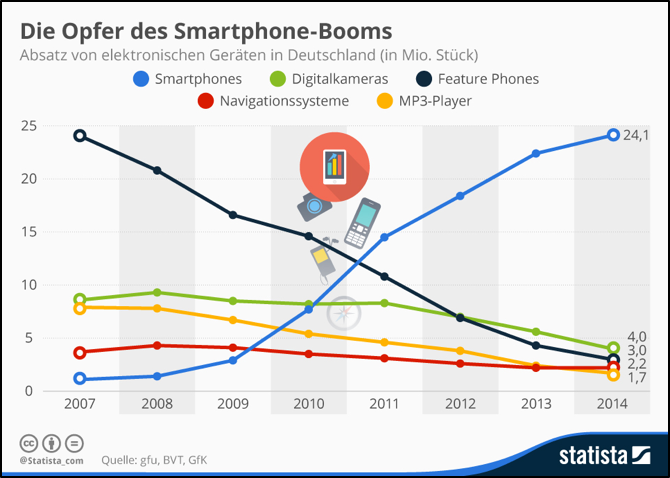
\includegraphics[scale=1.2]{./images/1.png}
\caption{Opfer des Smartphone-Booms \cite{SmartphoneBooms}}
\label{boom_opfer}
\end{center}
\end{figure}
Die Grafik \ref{boom_opfer} zeigt, wie die Smartphones eine immer größere Rolle spielen. Das liegt insbesondere daran, dass Smartphones in der Lage sind viele der Funktionen out-of-the-box zu erfüllen, oder mit Applikationen die Funktionalität nachträglich zu installieren \cite{zhou2011taming}. Da der Videokonsum auf den bis 2010 sehr kleinen Smartphone Bildschirmen nur bedingt befriedigend war, wurde mit dem iPad versucht, dieses Problem zu lösen. In Abbildung \ref{absatz_markt} ist der weltweite Absatz quartalsweise seit Q2 2010 abgebildet. Es ist deutlich zu sehen, wie der Absatz bis einschließlich 2012 stark gewachsen ist und sich seither auf einem nur leicht sinkenden Niveau hält.
\begin{figure}[h]
\begin{center}
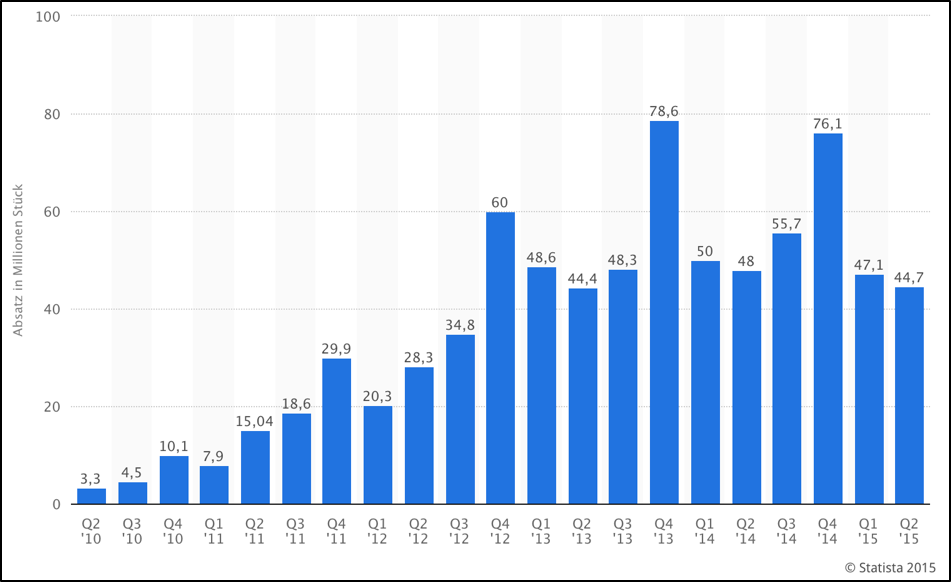
\includegraphics[scale=0.9]{./images/2.png}
\caption{Weltweiter Tablet Absatz \cite{AbsatzvonTablets}}
\label{absatz_markt}
\end{center}
\end{figure}
Die stark erhöhten Absätze jeweils im vierten Quartal sind insbesondere auf das Weihnachtsgeschäft zurückzuführen \cite{AbsatzvonTablets}. Apple ist mit dem iPad auf dem Tablet-Markt seit seiner Einführung Marktführer. Alleine im dritten Quartal 2015 wurden knapp 10 Millionen Geräte weltweit verkauft und erreicht somit einen Marktanteil von 20,3\%. Auf dem zweiten Platz liegt der Koreanische Elektronikhersteller Samsung mit einem Marktanteil von 16,5\%. Im Vergleich zum Vorjahr ist die Gesamtverkaufsmenge im dritten Quartal generell etwas geringer, die Marktanteile haben sich jedoch kaum verändert. \cite{IDCWorldwideQuarterlyTabletTracker} Analysten gehen jedoch davon aus, dass sich in den kommenden Jahren die Marktanteile weiter zugunsten von Microsoft mit ihren Windows-Tablets verschieben werden, da diese verglichen zu Android und iOS Geräten eher die Funktionen eines vollwertigen Laptops ersetzen können. Im Jahr 2015 liegt der Windows Marktanteil bei etwa 7\% und soll laut Prognose im Jahr 2019 bei etwa 14,1\% liegen.
\begin{figure}[h]
\begin{center}
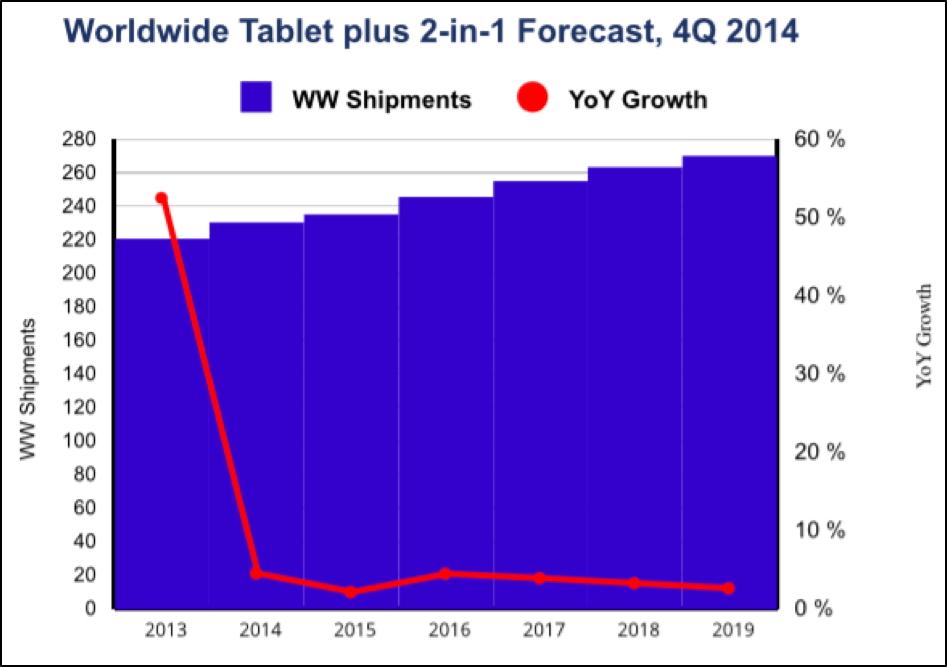
\includegraphics[scale=0.9]{./images/41.png}
\caption{Prognostizierte Marktentwicklung von Tablets bis 2019 \cite{IDCMarketdevelopment}}
\label{marktentwicklung}
\end{center}
\end{figure}
Generell geht die International Data Corporation davon aus, dass die weltweiten Verkaufszahlen sich bis 2019 konstant auf etwa 250 Millionen verkauften Tablets fixieren und sich das jährliche Marktwachstum einstellen wird. Diese Entwicklung ist auch in Abbildung \ref{marktentwicklung} in einem Diagramm dargestellt. \cite{IDCMarketdevelopment}
Das iPad war in erster Linie für den Privatgebrauch gedacht, jedoch haben seither auch Unternehmen großes Interesse an dieser Gerätekategorie gezeigt und evaluiert, wie diese Geräte den Alltag der Angestellten vereinfachen können, was insbesondere auf die hohe Mobilität zurückzuführen ist. Aus diesem Grund kommen die Nutzer sowohl aus dem Unternehmerbereich, sowie aus dem Privatsektor. In Schulen und Universitäten haben Tablet-PCs auch eine große Verbreitung gefunden. Technologiegestütztes Lernen kann die Leistung von Schülern und Studenten fördern, da die aktive Einbindung den Lernprozess unterstützt. Des Weiteren erhöht es die Interaktionsaktivität zwischen den Lehrern und Schülern. \cite{fischer2012potential}

Die sehr hohe Konsumentenanzahl von Videomedien macht es deshalb interessant, die Art und Weise, wie das Medium konsumiert wird, zu analysieren und Vorschläge zu machen, wie diese Erfahrung verbessert werden kann.

\section{Multimediale Inhalte}

Der Begriff Medium bedeutet im Allgemeinen Informationsträger. So können Informationen, die in unterschiedlichster Form existieren, gespeichert, transportiert und verbreitet werden. Beispiele dafür sind Video, Audio, Text und Bilder \cite{steinmetz2013multimedia}. Auf Tablets kann man viele unterschiedliche Arten von Medien konsumieren. Die hochauflösenden Bildschirme können Text so scharf darstellen, dass Bücher und Magazine selbst bei Dunkelheit angenehm gelesen werden können. Zusätzlich werden vollkommen neuartige Formen der Präsentation gegeben. Die Inhalte können nun auch mit Audio- und Videomaterial so kombiniert werden, sodass für den Nutzer ein tatsächlicher und unkomplizierter Mehrwert kreiert wird \cite{kallinen2011effects}. Doch nicht nur textueller Inhalt wird vermehrt auf mobilen Geräten mit berührungsempfindlichen Bildschirmen konsumiert, sondern auch Videos und Musik. Prinzipiell besteht multimedialer Inhalt aus zwei verschiedenen Komponenten. Zum einen ist das ein statischer Inhalt, wie beispielsweise ein Foto, was zu jedem gegebenen Zeitraum gleich ist. Zum anderen gibt es noch dynamische Inhalte, die sich zeitabhängig verändern, wie beispielsweise Animationen, audiomediale Inhalte und Videos. Darüber hinaus wird zwischen visuellen und nicht-visuellen Medien unterschieden. Visuelle Medien sind für den Betrachter sichtbar, wie Standbilder und Bewegtbilder. Dem gegenüber stehen die nicht-visuellen Medien wie Tonaufnahmen. Sobald mindestens zwei Medien miteinander kombiniert werden spricht man von Multimedia, wobei mindestens eines der Medien zeitbasiert, also kontinuierlich, sein muss. Ein klassisches Beispiel hierfür ist ein Spielfilm, bei dem sowohl Audio und Video zu einem Stream zusammengeführt werden.
\begin{figure}[h]
\begin{center}
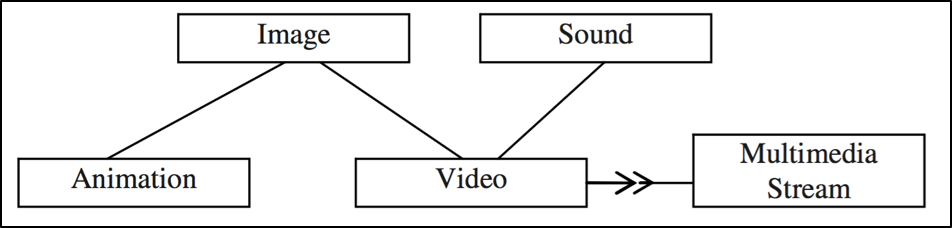
\includegraphics[scale=0.9]{./images/3.png}
\caption{Objektorientierte Darstellung von Medientypen \cite{reveiu2007using}}
\label{medien_objekt}
\end{center}
\end{figure}
In Grafik \ref{medien_objekt} ist veranschaulicht wie verschiedene Medienarten miteinander kombiniert werden, zu einem Multimedia Stream. Die Abbildung gibt hier als Beispiel ein Video an, welches mit einer Audiospur unterlegt ist \cite{reveiu2007using}. Standardmäßig sind Tablets mit Programmen ausgestattet, um solche Videodateien abspielen zu können. Welche Probleme im Kontext von Navigation und Darstellung existieren und mit welchen Methoden versucht wird diese zu lösen, wird in den folgenden Kapiteln aufgearbeitet.

\section{Videokonsum auf mobilen Geräten}

Der Konsum von Videos auf mobilen Geräten unterscheidet sich sehr von dem auf Desktop-PCs. Viele Fernsehsender bieten mittlerweile ihr Programm auch als Applikation an, sodass durch die oftmals permanente Internetverbindung auch unterwegs auf diese Medien zugegriffen und konsumiert werden kann. Medienquellen wie iTunes auf dem iPhone bzw. iPad oder auch Google Play für Android-Geräte sind große Konkurrenten zu den feststehenden Fernsehgeräten. Problematisch wird es, das zufriedenstellende Konsumerlebnis von den klassischen Videomedien, auf den mobilen Sektor zu übertragen, das liegt insbesondere daran, dass mobiler Videokonsum sich anders in den Alltag integriert \cite{o2007consuming}. Die Datenmengen, die über mobile Netzwerke konsumiert werden, sind heutzutage durch schnelle Internetanbindungen besonders hoch. Laut Cisco wird bis 2018 knapp 80\% des weltweiten Datenverkehrs alleine durch Videostreaming erzeugt und bis dahin der mobile Datenverkehr in Bezug auf Volumen, den von kabelgebundenen Geräten überholt haben. Im Jahr 2013 lag dieser Wert zum Vergleich noch bei 66\%. Plattformen wie YouTube und Netflix tragen hierbei eine ausschlaggebende Rolle, da Personen aufgrund von Bequemlichkeit diese Produkte eher auf Tablets und Smartphones konsumieren. Die Nutzer legen mittlerweile viel mehr Wert auf die Qualität der gelieferten Videos. Die Standardauflösung eines Fernsehers reicht daher oftmals nicht mehr aus, sondern Auflösungen wie \emph{FullHD}, also 1920x1080 Pixel, und sogar \emph{UltraHD} was der 4-fachen Auflösung von FullHD entspricht, also 3840x2160 Pixel, werden heute von den meisten Streamingportalen unterstützt. Die hohen Displayauflösungen der mobilen Geräte haben diesen Bedarf aufkommen lassen. Daraus resultieren mehrere Herausforderungen, die es zu bewältigen gilt. Zum einen ist das die Bereitstellung der Videos auf zuverlässiger Weise, was bedeutet, dass insbesondere bei Videostreams das Video möglichst ohne Unterbrechungen bei Konsumenten ankommt und das bei einer gleichbleibend hohen Qualität. Zum anderen müssen diese Videos benutzerfreundlich wiedergeben werden, was dann von den Applikationen umgesetzt werden muss. Der Bereich, der sich mit dieser Thematik beschäftigt wird auch \emph{Quality of Experience}, kurz QoE, genannt. \cite{sunqoe}

Der Fokus dieser Arbeit liegt aber in der Durchsuchbarkeit und Darstellung der Inhalte, was in den folgenden Kapiteln weiter erörtert wird.

\section{Durchsuchbarkeit von Multimedia Dateien}

Große Videobibliotheken sowie lange Videos werden oft zum Problem, was die inhaltliche Suche betrifft. Wenn man nicht weiß wo sich eine Datei befindet oder wie diese inhaltlich strukturiert ist, kann dies den Nutzer frustrieren. Im Vergleich dazu können bei textuellen Inhalten wie digitale Bücher einfache Suchanfragen gestartet werden, ohne dass der Nutzer komplizierte Suchanfragen erstellen muss. Große Texte können daher entweder mit Hilfe eines vorhandenen Index durchsucht werden, wie einem Inhaltsverzeichnis, oder auch mit einer Volltextsuche. Bei Videos können solche Suchanfragen, auch Queries genannt, nicht formuliert werden, weshalb manuell durchsucht werden muss und dies unter Umständen äußerst zeitaufwendig sein kann. Dazu kommt noch, dass Nutzer aufgrund der enormen Datenmengen oft gar nicht wissen, wie sie das Objekt, das sie gerne finden würden, in einer Suchanfrage beschreiben sollen \cite{schoeffmann20143}. In der Regel werden die Videos mit Metadaten ergänzt, sowie Tags, also Schlüsselwörter, die den Inhalt des Videos in irgendeiner Weise logisch beschreiben. So lassen sich jedoch keine bestimmten Szenen textuell beschreiben, sodass der Videoplayer automatisch zur gesuchten Stelle springt. Kollaborativ werden solche Tags auch von mehreren Nutzern gesetzt, damit diese Annotation auch zeitbezogen geschieht. Diese Technik wird auch \emph{Social Tagging} genannt. Ein Beispiel für ein solches System ist das Videoportal \emph{Yovisto} \cite{YovistoHomepage}, auf dem Videos aus akademischen Vorlesungen verfügbar sind. Der Videoplayer bietet verschiedene Möglichkeiten, um die Videos durchsuchbar zu machen. Neben dem klassischen Schieberegler, welcher die aktuelle Position der zu sehenden Szene in Relation zur Gesamtlänge zeigt, gibt es noch eine Tagging Box. Diese Tagging Box beinhaltet Schlagwörter, die die Nutzer passend zum Inhalt des Videos eingetragen haben. Da jeder Nutzer dieses Videoportals solche Annotationen machen kann, werden diese, im Falle von Wiederholungen entsprechend gewichtet. Daher sind Schlagworte mit häufigerem Vorkommen größer dargestellt, als Worte, die weniger oft genannt wurden. Die Abbildung \ref{yovisto} zeigt eine solche Tagging Box.
\begin{figure}[h]
\begin{center}
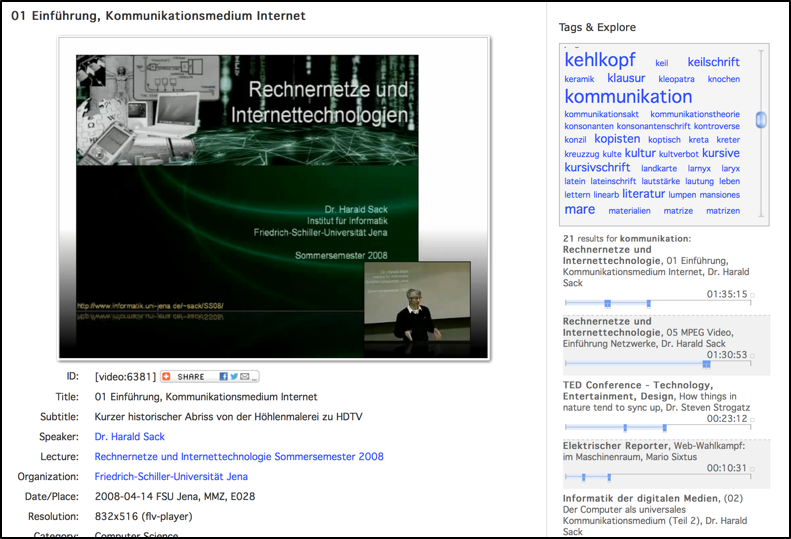
\includegraphics[scale=1.1]{./images/4.png}
\caption{Yovisto mit Tagging Box \cite{YovistoHomepage}}
\label{yovisto}
\end{center}
\end{figure}
Mit einem Klick auf eines der Schlagwörter öffnet sich darunter eine Liste mit Videos, in denen dieses Schlagwort annotiert wurde und jeweils an welchen Stellen im zeitlichen Verlauf der Videos. Von dort aus ist es dann möglich direkt zu der markierten Stelle zu springen, um sich den Inhalt anzusehen. Um das Thema oder den Inhalt des Videos schneller zu überblicken, werden unterhalb des Videos noch Metadaten wie der Name des Vortragenden, Aufnahmedatum, Untertitel, sowie der Name der Universität aufgelistet. \cite{gaiser2008good}

\section{Grundlagen der iOS Entwicklung}

Die Entwicklung für iOS Geräte unterscheidet sich von Desktopanwendungen dahingehen, dass von Beginn die eingeschränkten Ressourcen mit einkalkuliert werden müssen. Um Applikationen für Apple’s mobiles Betriebssystem entwickeln zu können, müssen unterschiedliche Paradigmen verstanden werden. Die wichtigsten Konzepte, die für die Umsetzung des Flickplayers relevant sind, werden in diesem Kapitel behandelt.

\subsection{Model-View-Controller Konzept}

Eines der wichtigsten Paradigmen in der iOS Entwicklung ist das Model-View-Controllers Entwurfsmuster, da es tief in Cocoa Touch verwurzelt ist. Cocoa Touch umfasst das gesamte Framework, um iOS Applikationen zu entwickeln. Teile einer Applikation können in drei unterschiedlichen Kategorien eingeteilt werden, welche Model, View und Controller sind. Das Model beschreibt die Datenschicht, also alle Daten, die dem Programm zur Verfügung stehen und bearbeitet werden. In dieser Schicht ist man einzig und allein auf die Daten fokussiert, was bedeutet, dass man hier keine Informationen darüber speichert, wie diese Daten später dargestellt werden. Beispielsweise kann dies eine Datenbank sein, welche Teil der Applikation ist. Modelle werden in der Regel als Unterklasse von NSObject erstellt, mit Instanzvariablen und Methoden, um deren Werte zu manipulieren. Die Visualisierung, also die Benutzeroberfläche, gehört zur sogenannten View. Auch hier wird sich nur auf diese eine Aufgabe beschränkt und keine Logik implementiert, die zur Abspeicherung der Daten benötigt wird. Die Kommunikation zwischen dem Model, also den Daten und der View wird vom Controller übernommen. Wenn sich beispielsweise die Daten ändern, dann wird auf dieser Ebene die Benutzeroberfläche darüber informiert, sodass diese sich dementsprechend anpassen muss. Wenn das Datenmodell besonders einfach ist, dann ist es dennoch möglich diese als Teil des Controllers zu implementieren, sodass keine zusätzliche Klasse dafür angelegt werden muss. In der iOS Entwicklung werden die Controller als Unterklasse von UIViewController angelegt.
\begin{figure}[h]
\begin{center}
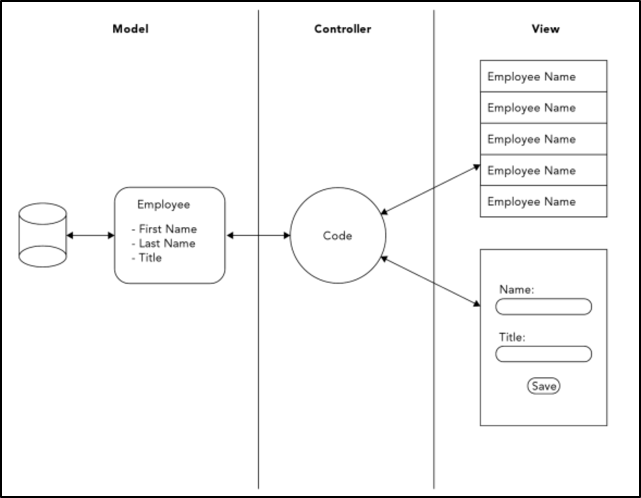
\includegraphics[scale=1.1]{./images/19.png}
\caption{Model-View-Controller \cite{harris2014beginning}}
\label{model_view_controller}
\end{center}
\end{figure}
In Abbildung \ref{model_view_controller} ist das Konzept des Model-View-Controllers grafisch veranschaulicht. In diesem Beispiel gibt es eine Datenbank, welche eine Menge von Mitarbeitern verwaltet. Des Weiteren können die existierenden Mitarbeiter aufgelistet werden, sowie neue Mitarbeiter angelegt werden. Die strikte Modularisierung ist hier sehr gut zu sehen, da die View beispielsweise nur das Eingabeformular und einen Knopf zum Abspeichern anzeigt. Was mit den eingegeben Werte passiert, bzw. was generell passieren soll, wenn dieser Knopf gedrückt wird, wird allein vom Controller übernommen. Nach einer Aktion sind die neuen Daten ebenfalls nur in dem Model zu finden und nicht im Controller selbst. Der besondere Vorteil dabei ist, dass die Daten unabhängig verwaltet werden und so verschiedene Controller unterschiedliche Aufgaben übernehmen können. \cite{harris2014beginning}

Da die Kommunikation zwischen der View und dem Model nie direkt passiert, müssen Benachrichtigungen mit sogenannten Protokollen und Delegates implementiert werden. Das folgende Kapitel gibt einen kurzen Überblick, welche Bedeutung diese in der iOS Entwicklung haben und wie sie umgesetzt werden.

\subsection{Protokolle und Delegates}

Protokolle und Delegates kommen dann zum Einsatz, wenn komplexe Kommunikation zwischen zwei Objekten gefordert ist. Die Verwendung von Delegates und Protokollen ist für die iOS Entwicklung essentiell und ist daher Teil der Grundlagen. Um dieses Konzept zu verstehen, lässt es sich am besten an einem Beispiel erklären. Eine TableView, also eine Liste mit mehreren Einträgen, durch die man navigieren kann, ist Teil eines Controllers. Die TableView soll eine Übersicht von Fotos haben und mit einem Tipp auf ein einzelnes Foto soll dieses vergrößert dargestellt werden. Die TableView besitzt eine Vielzahl von Methoden, die beispielsweise erkennen, auf welche Zelle getippt wurde oder auch ob der Nutzer durch die Liste navigiert. Da eine TableView aber nicht in jedem Fall in gleicher Weise darauf reagieren soll, wird die eigentliche Funktionalität von den referenzierten Objekten implementiert. Die Funktionen werden innerhalb der TableViews mit Protokollen definiert, die an den entsprechenden Stellen aufgerufen werden. Des Weiteren hat die TableView ein sogenanntes Delegate-Property, welches vom Typ des Protokolls ist. Auf diesem Delegate-Objekt werden dann innerhalb der TableView-Klasse die Protokoll-Methoden aufgerufen. Wenn die TableView nun vom Controller initialisiert wird, dann wird der Controller zum Delegate dieser TableView-Instanz gesetzt. Dazu muss der Controller die Methoden, oder nur diejenigen, die auch tatsächlich benötigt werden, implementieren, um konform zum Protokoll zu sein. Wenn der Nutzer nun auf ein verkleinertes Foto in der Liste tippt, dann ruft die TableView die entsprechende Delegate-Methode auf und übergibt dieser die Position der Zelle. Da die Implementierung dieser Methode vom Delegate gemacht wird, in diesem Fall dem Controller, kann darin auf die Interaktion reagiert werden und mit der Information über die ausgewählte Zelle das entsprechende Foto vergrößern. Protokolle und Delegates werden nicht nur von Klassen aus dem iOS SDK eingesetzt, sondern können und sollten auch von eigenen Klassen umgesetzt werden. Der besondere Vorteil dieses Entwurfsmuster ist, dass sich so weitere Ableitungen der TableView-Klasse vermeiden lassen und sich so Beziehungen zwischen jeglicher Art von Klassen aufbauen lassen. Eine Kapselung der Logik wird so konsequent etabliert und die Logik nur dort implementiert, wo die konkreten Informationen auch verarbeitet werden. \cite{appsfuerios} \cite{WorkingwithProtocols}

\subsection{Observerpattern}

Neben den Protokollen und Delegates ist das Observer Entwurfsmuster ein ebenso wichtiger Bestandteil aus der Programmierung für iOS, um Benachrichtigungen bzw. Kommunikation zwischen mehreren Objekten umzusetzen. Der grundlegende Gedanke dahinter ist, das an unterschiedlichen Stellen im Programm auf bestimmte Ereignisse reagiert werden muss. Wie auf diese Ereignisse reagiert wird, ist in diesem Fall zweitrangig. Prinzipiell haben zwei Arten von Observern einen besonderen Stellenwert in der iOS Entwicklung, welche zum einen die Notifications und zu anderen der Key-Value Observer sind. Die iOS Foundation bietet mit der NSNotificationCenter Klasse ein mächtiges Werkzeug, um mit solchen Benachrichtigungen umzugehen. Die grundlegende Idee dahinter ist, dass ein Objekt eine Notification hinzufügen kann, welche einen Namen hat. Das NSNotificationCenter bietet mit dem defaultCenter() eine Singleton Instanz, welche diese dann verwaltet. Um neue Benachrichtigungen hinzuzufügen, muss folgende Methode verwendet werden:
\begin{lstlisting}
- (id<NSObject>)addObserverForName:(NSString*)name
                            object:(id)obj
                             queue:(NSOperationQueue *)queue
                        usingBlock:(void (^)(NSNotification *note))block
\end{lstlisting}
Andere Objekte können sich nun zu diesem Observer anmelden und eine Funktion implementieren, die ausgeführt wird, wenn zu dieser Notification ein Post ausgelöst wurde. Das Anmelden zu einer gegebenen Notification wird mit folgender Methode ausgeführt:
\begin{lstlisting}
-(void)addObserver:(id)notificationObserver
          selector:(SEL)notificationSelector
              name:(NSString *)notificationName
            object:(id)notificationSender
\end{lstlisting}
Der Post, um alle Subscriber zu benachrichtigen, wird vom Objekt durchgeführt, welche die Notification erstellt hat. Folgende Methode muss dafür implementiert werden:
\begin{lstlisting}
- (void)postNotificationName:(NSString *)notificationName
                      object:(id)notificationSender
\end{lstlisting}
Man kann diese Art von Observern wie mit einem Newsletter vergleichen. Ein Dienst schickt einen Newsletter an alle Personen aus, die sich für diesen angemeldet haben. Der Dienst an sich macht hierbei keinen Unterschied darin, wie die einzelnen Personen darauf reagieren. Innerhalb von iOS werden viele dieser Notifications verwendet, wie beispielsweise von der Tastatur, die eine Notification postet, sobald diese zum Vorschein kommt oder wieder geschlossen wird. Auch andere Applikationsbenachrichtigung werden sehr häufig benutzt, sodass eine Applikation darauf reagieren kann, wenn sie in den Hintergrund geschoben wird. Bei Videoplayern wird dies in der Regel benutzt, um das aktuelle Video zu pausieren, sodass es nicht im Hintergrund weiterläuft. \cite{NSNotificationCenterClass} \cite{chung2011pro}

Der Key-Value Observer hat eine besondere Bedeutung, da dieser unter anderem verwendet wird, um Benachrichtigung zwischen dem Model und dem Controller auszutauschen. Der Unterschied zur Notification ist hierbei, dass ein bestimmtes Attribut von einem Objekt überwacht wird und eine Benachrichtigung postet, sobald sich der Wert dieses Attributs ändern. Des Weiteren gibt es keine zentrale Stelle, die die Benachrichtigungen verwaltet. Mit Hilfe des folgenden Beispiels wird dieses Entwurfsmuster weiter erklärt. Es gibt zwei Objekte, das BankObject und das PersonObject. Das BankObject besitzt ein Attribut accountBalance, welches den aktuellen Kontostand einer Person wiederspiegelt.
\begin{figure}[h]
\begin{center}
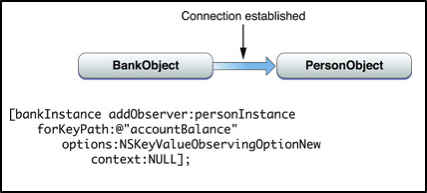
\includegraphics[scale=1.2]{./images/20.png}
\caption{Key-Value Observer anlegen \cite{KeyValueObserving}}
\label{keyvalue_anlegen}
\end{center}
\end{figure}
Die Instanz des BankObject fügt nun einen Observer hinzu, siehe Abbildung \ref{keyvalue_anlegen}, welcher die Instanz des PersonObject benachrichtigt, sobald sich das Attribut accountBalance ändert. Wie die Instanz des PersonObject darauf reagiert, muss in der Klasse dieser definiert werden.
\begin{figure}[h]
\begin{center}
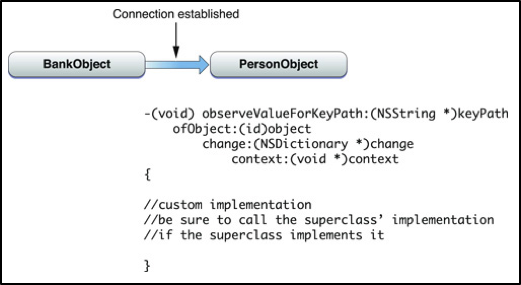
\includegraphics[scale=1.2]{./images/21.png}
\caption{Key-Value Observer anmelden \cite{KeyValueObserving}}
\label{keyvalue_anmelden}
\end{center}
\end{figure}
Dazu muss die Methode in Abbildung \ref{keyvalue_anmelden} implementiert werden. Der Methodenblock wird dann ausgeführt, sobald sich der Wert ändert. Der Vorteil hierbei ist, dass Benachrichtigungen nicht aktiv versendet werden müssen und Objekte ohne weitere Klassen miteinander verbunden werden und Informationen austauschen können. \cite{KeyValueObserving} \cite{learnios8}

\subsection{AVFoundation}

Für die Entwicklung des Flickplayers musste ein geeignetes Framework ausgewählt werden, welches in der Lage ist, Videos während der Laufzeit zu manipulieren. Das iOS SDK bietet mit der AVFoundation ein leistungsstarkes Framework, welches in der Lage ist, audiovisuelle Daten, also Ton- und Videoaufnahmen, zu erzeugen, editieren, untersuchen und selbstverständlich auch abzuspielen. Des Weiteren gibt es Klassen, die speziell den Umgang Audio implementieren.
\begin{figure}[h]
\begin{center}
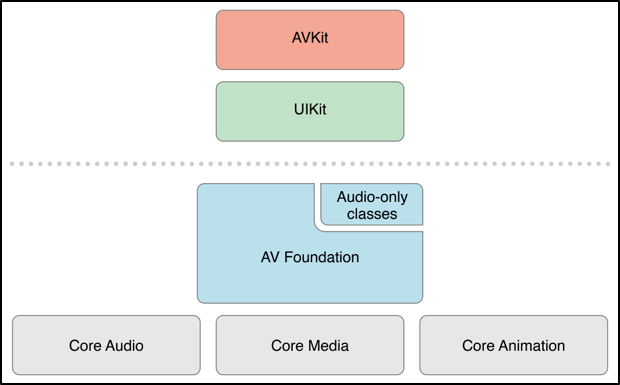
\includegraphics[scale=1.1]{./images/22.png}
\caption{Einordnung von AVFoundation in iOS \cite{AboutAVFoundation}}
\label{AVFoundation}
\end{center}
\end{figure}
In Abbildung \ref{AVFoundation} ist zu sehen, wie die AVFoundation in iOS integriert wurde. Das Framework verwendet Methoden aus aus Core Audio, Core Media und Core Animation, welche zu den low-level Frameworks zählen \cite{AboutAVFoundation}. Core Audio übernimmt hier beispielsweise alle Aufgaben, um die Audiodaten zu handhaben und Core Media unterstützt die AVFoundation mit dem Umgang von zeitbasierten Aktionen rund um CMTime \cite{mccune2014learning}. Für das Abspielen eines Videos werden drei Komponenten benötigt. Zum einen ist dies ein AVAsset, also die eigentliche Datei, die abgespielt werden soll. Da dieses Objekt nicht direkt abgespielt werden kann, muss es einem AVPlayerItem übergeben werden, da dies den aktuellen Status des Videos repräsentiert. Der AVPlayer ist dann der eigentliche Videoplayer, welcher alle Methoden zur Verfügung stellt, um das Video zu steuern. Dies sind beispielsweise einfache Funktionen, wie das Starten und Pausieren des Videos.
\begin{figure}[h]
\begin{center}
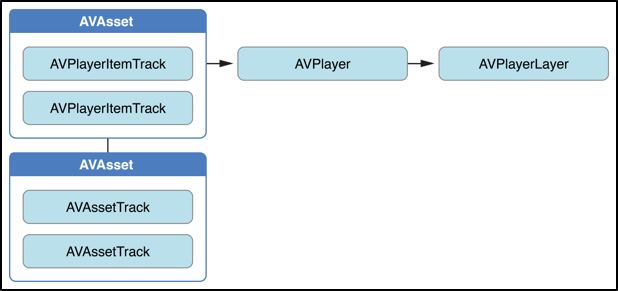
\includegraphics[scale=1.1]{./images/23.png}
\caption{Abspielen einer Videodatei mit AVFoundation \cite{AVFoundationPlayback}}
\label{play_with_avfoundation}
\end{center}
\end{figure}
Um das Video für den Nutzer anzuzeigen, muss die AVPlayer-Instanz einem AVPlayerLayer übergeben werden, welcher dann in einer UIView angezeigt werden kann. In der Abbildung \ref{play_with_avfoundation} sind die Referenzen zwischen den einzelnen Komponenten in einem Diagramm grafisch dargestellt. Da die eigentliche Datei, das AVAsset, nicht direkt abgespielt wird, sondern den Wrapper AVPlayerItem verwendet, kann eine Datei von unterschiedlichen AVPlayern gleichzeitig abgespielt werden und somit das auch Rendering unterschiedlich sein kann. Das Manipulieren der Abspielgeschwindigkeit während der Laufzeit ist für den Flickplaner eine essentielle Funktionalität. Der AVPlayer hat hierfür ein Attribut \textit{rate}, welches zu jedem Zeitpunkt verändert werden kann. Das geht sowohl zum Beschleunigen, zum Verlangsamen, sowie zum rückwärts Abspielen des Videos. All diese Funktionen sollten Teil des Flickplayers sein und somit auch angewendet werden. Dennoch gibt es hier Limitierungen, welche in den folgenden Kapiteln genauer beleuchtet werden. \cite{AVFoundationPlayback}

\subsection{Gesturerecognizer und UIResponder}
\label{sec:Gesturerecognizer}

Fehlende Peripherie wie Maus und Tastatur, zumindest als Hardware, wird bei mobilen Geräten durch einen Berührungsempfindlichen Bildschirm ersetzt. Das iOS SDK bietet viele Schnittstellen, um auf Berührungen und Gesten reagieren zu können. Nicht jedes Objekt kann auf Eingaben reagieren, denn dazu muss es eine Unterklasse von UIResponder sein. Generell gibt es hier zwei unterschiedliche Ereignisse, welche zum einen ein Berührungsereignis und zum anderen ein Bewegungsereignis sind. Das Berührungsereignis gibt an, dass eine Berührung mit einem Objekt gerade begonnen oder aufgehört hat. Eine Berührung ist zu Ende, sobald der Nutzer den Finger wieder anhebt. Für die Implementierung der Flickplayers ist diese Art von Interaktionserkennung besonders wichtig, da aus diesen Informationen der Benutzereingabe die Interaktion erst möglich wird \cite{UIResponderClass}. Die sogenannte Responder Chain, siehe Abbildung \ref{uiresponderchain}, also eine Kette, macht es möglich, Ereignisse durch eine Hierarchiekette weiterzugeben.
\begin{figure}[h]
\begin{center}
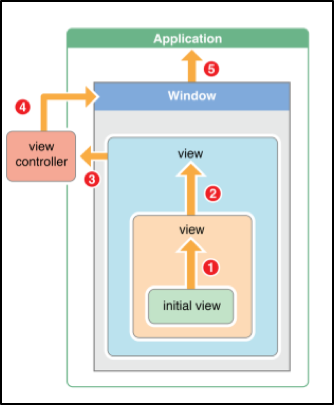
\includegraphics[scale=1.1]{./images/24.png}
\caption{UIResponder Chain \cite{UIResponderChain}}
\label{uiresponderchain}
\end{center}
\end{figure}
Der Sinn dahinter ist, dass ein visuelles Objekt, in der Regel eine UIView oder eine Unterklasse davon, ein Event entgegennimmt und nicht selbst darauf reagiert. Das Event wird von der UIView in der Hierarchie weitergegeben und dann von dem Objekt verarbeitet, welches die Protokollmethoden implementiert \cite{UIResponderChain}. Vordefinierte Arten von Gesten können mit einem sogenannten UIGestureRecognizer direkt einem UIView zugewiesen werden. Jede Unterklasse von UIGestureRecognizer befähigt den Umgang mit genau einer Gesteninteraktion. Die einzelnen Gesten, die vom iOS SDK zur Verfügung gestellt werden, sind im Folgenden aufgelistet.
\begin{itemize}
\item UITapGestureRecognizer
\item UIPinchGestureRecognizer
\item UIRotationGestureRecognizer
\item UISwipeGestureRecognizer
\item UIPanGestureRecognizer
\item UIScreenEdgePanGestureRecognizer
\item UILongPressGestureRecognizer
\end{itemize}
Diese sind einfache Gesten, wie die Tap-Geste, oder auch auch die Pinch-Geste, die insbesondere verwendet wird, um ein Objekt zu vergrößern bzw. zu verkleinern. Zusätzlich kann hier noch angemerkt werden, dass eine Instanz mehrere Attribute besitzt, welche beispielsweise angeben, mit wie vielen Fingern die Geste ausgeführt werden muss, um als solche erkannt zu werden. Eine Instanz von UIView hat die Methode addGestureRecognizer, mit der man eine Instant der oben genannten GestureRecognizer hinzufügen kann. Des Weiteren benötigt die Methode einen Selector, welcher ausgeführt wird, wenn der Nutzer diese Geste auf dem Objekt gemacht hat. \cite{UIGestureRecognizerClass}

In diesem Kapitel wurden die Grundlagen aufgearbeitet, um die Implementierung des Flickpayers möglich zu machen. Wie der Prototyp im Detail umgesetzt wurde, wird in Kapitel 5 behandelt. Im folgenden Kapitel wird ganze Thematik von Videobrowsing detailliert erörtert.

\chapter{Videobrowsing}

Im vorherigen Kapitel hat sich herauskristallisiert, dass sich multimediale Dateien nicht ohne Weiteres durchsuchen lassen, jedenfalls nicht, wenn man eine vollständig manuelle Suche vermeiden möchte. Das Gebiet des Videobrowsings beschreibt die Aufgabe sich durch ein Video zu navigieren, um eine oder mehrere Szenen zu finden, oder einen Überblick über den Inhalt zu bekommen. Daher gibt es die Möglichkeiten den Inhalt zu analysieren und grafisch aufzubereiten, die Darstellung und Navigation an sich zu ändern, oder beide Methoden miteinander zu kombinieren \cite{juengling2014videozoom}. In diesem Kapitel werden deshalb Methoden vorgestellt, die eine oder beide dieser Konzepte einsetzten.

\section{Navigationsunterstützung}

Im Bereich der Videoplayer wurden bisher einige Versuche gemacht, die Navigation zu vereinfachen, sodass auch Nutzer ohne besondere Vorkenntnisse das Werkzeug bedienen können. Insbesondere bei mobilen Geräten wie Smartphones und Tablets gibt es nur wenige Alternativen zur klassischen Bedienoberfläche. Die geringe Leistung und der Formfaktor, also die geringe Bildschirmgröße, spielen hier eine nicht unerhebliche Rolle \cite{fan2003visual}.

\subsection{Klassische Navigation}

Mit der Einführung von Videorekorder, engl. Video Cassette Recorder, wurde auch der Begriff VCR controls etabliert. Diese beschreiben die Standardeingabemethoden, um mit dem Videorekorder kommunizieren zu können. Diese waren üblicherweise Knöpfe, welche Funktionen wie Start, Pause, vor- und zurückspulen und Stopp übernahmen. Dieses Konzept hat sich mittlerweile so stark bei den Nutzern eingeprägt, dass bei allen gängigen Video und Musikplayern dieses Konzept übernommen wurde. Dies wurde teilweise auch mit einer Zeitleiste kombiniert, sodass auch grafisch dargestellt wird, wo man sich momentan im Video befindet \cite{he2007supporting}. Als Beispiele zeigen die folgenden Abbildungen die Benutzeroberfläche zweier bekannter Videoplayer. Zum einen ist das der aktuelle \emph{YouTube} Player und zum anderen der \emph{VLC Media Player} in der Version 2.2.1. Sowohl der YouTube Player, als auch der VLC Media Player haben eine sehr ähnlich strukturierte Menüführung. Beide haben in der unteren linken Ecke den Start- bzw. Pause-Knopf, sowie die Möglichkeit zum nächsten Video in der Wiedergabeliste zu springen. Des Weiteren besitzen beide die besonders übliche Navigationsleiste, um sich schnell innerhalb des Videos zu bewegen.
\begin{figure}[h]
\begin{center}
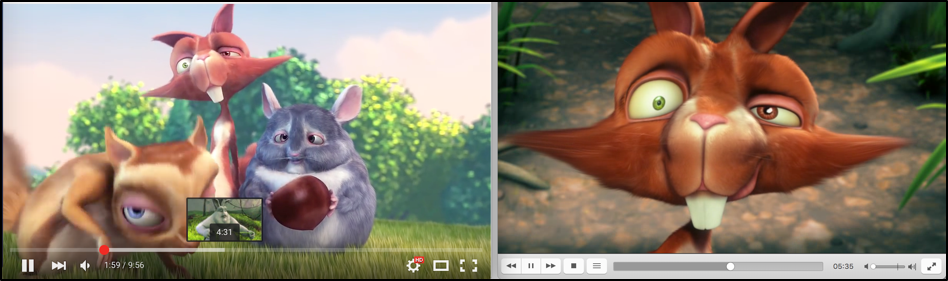
\includegraphics[scale=0.9]{./images/5.png}
\caption{Standardvideoplayer YouTube und VLC Player im Vergleich}
\label{youtube_vlc}
\end{center}
\end{figure}
In Ergänzung dazu hat der YouTube Player eine Funktion, bei der der Nutzer mit dem Mauszeiger über die Suchleiste geht und ohne zu klicken eine Vorschau dieser Stelle zu bekommen. Wenn der Nutzer aber eine bestimmte Szene finden möchte, aber nicht weiß an welcher Stelle sich diese befindet, ist diese Navigationsmethode unter Umständen weniger zufriedenstellend. Anhand eines Beispiels lässt sich das Problem von Zeitleisten-basierten Videoplayern besser hervorheben. Ein Fußballspiel wird live übertragen und während der Halbzeitpause kann man die vergangene Spielhälfte nochmals zur Analyse abspielen lassen. Für den Zuschauer sind hier offenbar nur wichtige Szenen interessant, die einen Einfluss auf das Spielergebnis haben. Das sind vor allem Tore, Fouls oder Angriffe, die fast zu einem Tor geführt haben. Bei einem 45-Minuten langem Video würde eine manuelle Suche sehr zeitaufwendig sein, da man sich in der Regel die exakten Zeitpunkte nicht merken konnte.Es gibt Videoplayer, die es während der Wiedergabe eines Videos oder Streams ermöglichen, Markierungen zu setzen. Innerhalb der Halbzeitpause kann dann von einer Markierung zur nächsten navigiert werden, ohne sich unwichtige Stellen ansehen zu müssen. Die Granularität der Zeitleisten ist oftmals eher ungenau und lässt den Nutzer in Sekundenintervallen navigieren. Das liegt daran, dass bei besonders langen Videos die Zeitleiste aufgrund von Platzmangel auf dem Bildschirm nicht entsprechend skaliert werden kann. Die maximale Bewegungsgenauigkeit auf dem Bildschirm liegt bei einem Pixel. Die Distanz von einem Pixel zum nächsten ist daher bei kurzen Videos ebenfalls kürzer, gemessen an dem relativen Verhältnis zur Videolänge. Dies wird zum Problem, wenn man sich eine bestimmte Szene stark verlangsamt anschauen möchte, um eine detailierte Anaylse zu machen. Das ist zum Beispiel der Fall, wenn der Ball außerhalb des Spielfeldes gelangt und es nicht sicher ist, welcher Spieler den Ball zuletzt berührt hat. Auch hier müssen Videoplayer eingesetzt werden, die über die herkömmliche Funktionalität hinausgehen und beispielsweise eine Navigationsmethode implementieren, die eine Frame-by-Frame Navigation ermöglicht, die Zeitleiste skalierbar ist, oder das Video schlichtweg langsamer abspielen lässt. \cite{furht2009handbook}

In den folgenden Kapiteln werden noch weitere Tools vorgestellt, die diesen konventionellen Pfad verlassen und mit Hilfe von Inhaltsanalysen und interaktiver Videosuche diesen Vorgang beschleunigen und vereinfachen. 

\subsection{Automatische Inhaltsanalyse}

Bei sehr großen Ansammlungen von Multimediadaten ist eine manuelle Durchsuchbarkeit praktisch nicht gegeben. Mit Hilfe einer automatischen Inhaltsanalyse kann der Nutzer ein Video oder mehrere Videos nach bestimmten Merkmalen untersuchen, je nach dem was in dieser Situation am sinnvollsten ist. Dazu kommt noch, dass dieses Teilgebiet von Videobrowsing in der Regel nicht nur von Nutzern verwendet wird, die schnell eine bestimmte Szene innerhalb eines Videos finden möchten, sondern von Firmen die beispielsweise Videoüberwachungssysteme einsetzen. Denn hier steht man vor dem Problem, dass teilweise rund um die Uhr gefilmt wird und es dadurch unmöglich ist, bestimmte Aktivitäten aus dem Video hervorzuheben, die für den Überwacher von Bedeutung sind. Zum Beispiel kann ein solches Video auf Bewegungsaktivitäten untersucht werden, sodass man einfach und schnell von einer aktiven Szene zur anderen navigieren kann, ohne sich den uninteressanten Inhalt dazwischen anschauen zu müssen. Da heutige Systeme zwar schon sehr ausgereift sind, kann und wird man nicht vollkommen auf menschliche Begutachtung verzichten können. Die für den Betrachter interessanten Szenen zu erkennen ist eine Sache, jedoch müssen die von dem Videobrowser gelieferten Ergebnisse auch selbst einfach und in angemessener Zeit durchsuchbar sein \cite{ghosh2012discovering}. Daher ist eine grafisch sinnvolle Benutzeroberfläche des Tools ebenso auschlaggebend, wie der Algorithmus, der diese Ergebnisse produziert. Der ganze Vorgang wird auch Video Summarization genannt, da die wichtigen Inhalte aus dem langen Video zusammengefasst und aufbereitet werden \cite{ngo2005video} \cite{vasconcelos1998bayesian}. Im Folgenden werden verschiedene Tools vorgestellt:

Juengling, Blunsden und Versino haben den \emph{VideoZoom} vorgeschlagen. Veränderungen werden hier in zwei Phasen erkannt. Zuerst werden zur Laufzeit Änderungen von angrenzenden Bildern hervorgehoben. Dies wird in der zweiten Phase mit einem Algorithmus kombiniert, welcher die Schatten von den Objekten erkennt. So ist es möglich die interessanten Objekte zu markieren, was dann auch Tubes genannt wird. Im Anschluss kann man solche Tubes als Suchinformation übergeben und VideoZoom liefert eine Übersicht zurück, mit allen gefundenen Objekten. Mit einem Klick auf ein Ergebnis, welches ein Vorschaubild der Szene ist, navigiert man im originalen Video zur gesuchten Stelle. Im Fall der VideoZoom Studie lieferte insbesondere die Suche nach Fahrzeugen sehr genaue Ergebnisse. \cite{juengling2014videozoom}

Mit dem \emph{Video Explorer} von Schöffmann erlaubt es mit zwei Arten ein Video zu durchsuchen. Zum einen können gesuchte Features durch Histogramme visuell dargestellt werden und zum anderen kann das Video anhand von gegeben Beispielen durchsucht werden. Bis dahin konnte man Videosuchtools in drei verschiedene Klassen aufteilen. Zum einen ist das die textuelle Suche, bei der Schrift und Sprache innerhalb der Videos extrahiert wird und als Text zur Verfügung steht, womit sich dann gewöhnliche Textsuchen durchführen lassen. Die zweite Kategorie ist, dass man ein Beispielbild als Suchparameter verwendet. Problematisch ist jedoch, dass der Nutzer oftmals kein Beispiel zur Hand hat, das er verwenden kann. Als dritte Kategorie gibt es noch die konzeptuelle Suche, welche es erlaubt semantische Konzepte als Suchparameter zu übergeben. Das bedeutet, dass der Nutzer beispielsweise nach Strand sucht und alle Stellen im Video angezeigt werden, die einen Strand zeigen. Dies geschieht anhand von Deskriptoren, die Farbe, Texturen und Kompositionen innerhalb des Videos mit einem trainierten Machine Learning Algorithmus zusammenfassen und damit das Video durchsuchen können. Ein großes Problem dabei ist, dass die Analyse eines gegebenen Videos um ein vielfaches länger dauert, als die eigentliche Videolänge. Dazu kommt noch, dass die Navigationsoberflächen solcher Tools kaum intuitiv sind, was eine Suche noch zeitaufwendiger macht. Um dieses Problem zu lösen, implementiert der Video Explorer eine Farb- und Bewegungserkennung, die während der Dekodierung des Videos schnell durchgeführt werden kann und projiziert die Ergebnisse als Histogramme zu einer Zeitleiste, die gleichzeitig als Navigationsleiste dient, wie sie auch bei Standardvideoplayern verwendet wird. In der folgenden Abbildung 3.2 ist die Benutzeroberfläche des Video Explorers zu sehen, mit drei verschiedenen Features, nach denen gesucht wird. Da wären die Key Frames, dominante Farben und der Bewegungsverlauf innerhalb des Videos. Jedes einzelne Feature wird auf einer eigenen Suchleiste projiziert.
\begin{figure}[h]
\begin{center}
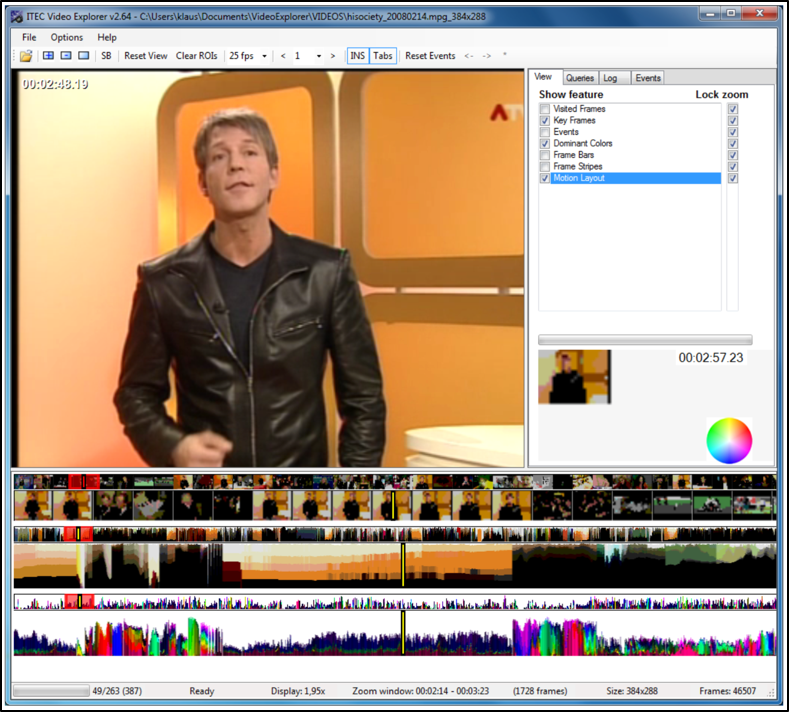
\includegraphics[scale=1]{./images/6.png}
\caption{Video Explorer mit verschiedenen Suchleisten \cite{schoeffmann2010video}}
\label{video_explorer}
\end{center}
\end{figure}
Anhand des gelben Balkens weiß der Nutzer sofort, wo er sich im Video gerade befindet. Im gezeigten Beispiel ist eine Nachrichtensendung zu sehen. Hier werden verschiedene Berichte abgespielt, die immer zuvor vom Nachrichtensprecher angekündigt werden. Da sich in der Regel innerhalb der selben Sendung die Kleidung und der Hintergrund des Sprechers nicht verändern, kann mit Hilfe der aktivierten Suche für die dominanten Farben immer sehr einfach auf der Navigationsleiste erkannt werden, wo ein Beitrag zu Ende ist und eine neuer Beitrag beginnt. Hier sind die dominanten Farben Orange und Schwarz sehr deutlich zu erkennen. Die Bewegungserkennung ist in diesem Fall auch sehr hilfreich, da sich der Nachrichtensprecher nicht viel bewegt und auch keine großen Kameraschwenker gemacht werden. Auf der Navigationsleiste für diese Suche werden Bewegungen ebenfalls durch Farben dargestellt, wobei Weiß bedeutet, dass keine Bewegung vorhanden ist. Eine weitere Eigenschaft des Video Explorers ist, dass man innerhalb der Navigationsleiste hereinzoomen kann.
\begin{figure}[h]
\begin{center}
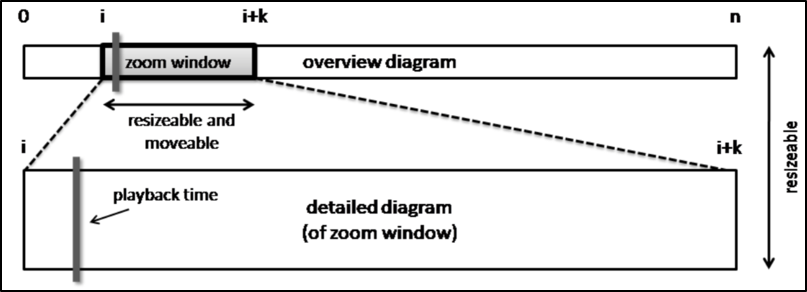
\includegraphics[scale=1.05]{./images/7.png}
\caption{Zoom innerhalb der Navigationsleiste beim Video Explorer \cite{schoeffmann2010video}}
\label{zoom_video_explorer}
\end{center}
\end{figure}
Das ist besonders hilfreich, wenn das Video etwas länger ist und man eine detailliertere Übersicht eine ausgewählte Sequenz bekommen möchte. Wie schon angesprochen unterstützt der Video Explorer auch eine Beispielsuche. Dafür wird ein gewünschter Bereich des Videos markiert und später dann durch den Player angezeigt, an welchen Stellen im Video dies das gesuchte Muster wiederholt. \cite{schoeffmann2010video}

Für Zielsuchaufgaben, bei denen der Nutzer voher schon weiß, wie die gesuchte Stelle aussieht, hat Bai et al. \cite{bai2013interactive} einen Videobrowser vorgeschlagen, der zu Beginn eine Videosammlung analysiert und Keyframes extrahiert. Die gewonnen Informationen werden in eine Datenbank gespeichert, die für die späteren Suchen herangezogen wird. Wenn ein Nutzer nun eine Szene finden möchte, dann wird die gesuchte Stelle als Suchparameter dem Suchsystem übergeben, welches passende Keyframes mit deren Zeitstempeln zurückliefert. Dieses Ergebnis wird dann vom Nutzer verwendet, um an die gesuchte Stelle zu navigieren.

Mit den Joke-O-Mat von Friedland et al. \cite{friedland2009joke} wurde ein Ansatz vorgestellt, bei dem die Audiospur einer Sitcom-Serie analysiert wird und auf dieser Grundlage verschiedene Szenen erkannt werden können. Die Analysealgorithmen können trainiert werden, sodass bestimmte Personen erkannt werden können und mit Hilfe der Zeitstempel dann zu denen Szenen springen kann, an denen die gesuchten Personen gerade Sprechen. In der folgen Abbildung ist die Benutzeroberfläche des Joke-O-Mat's dargestellt.
\begin{figure}[h]
\begin{center}
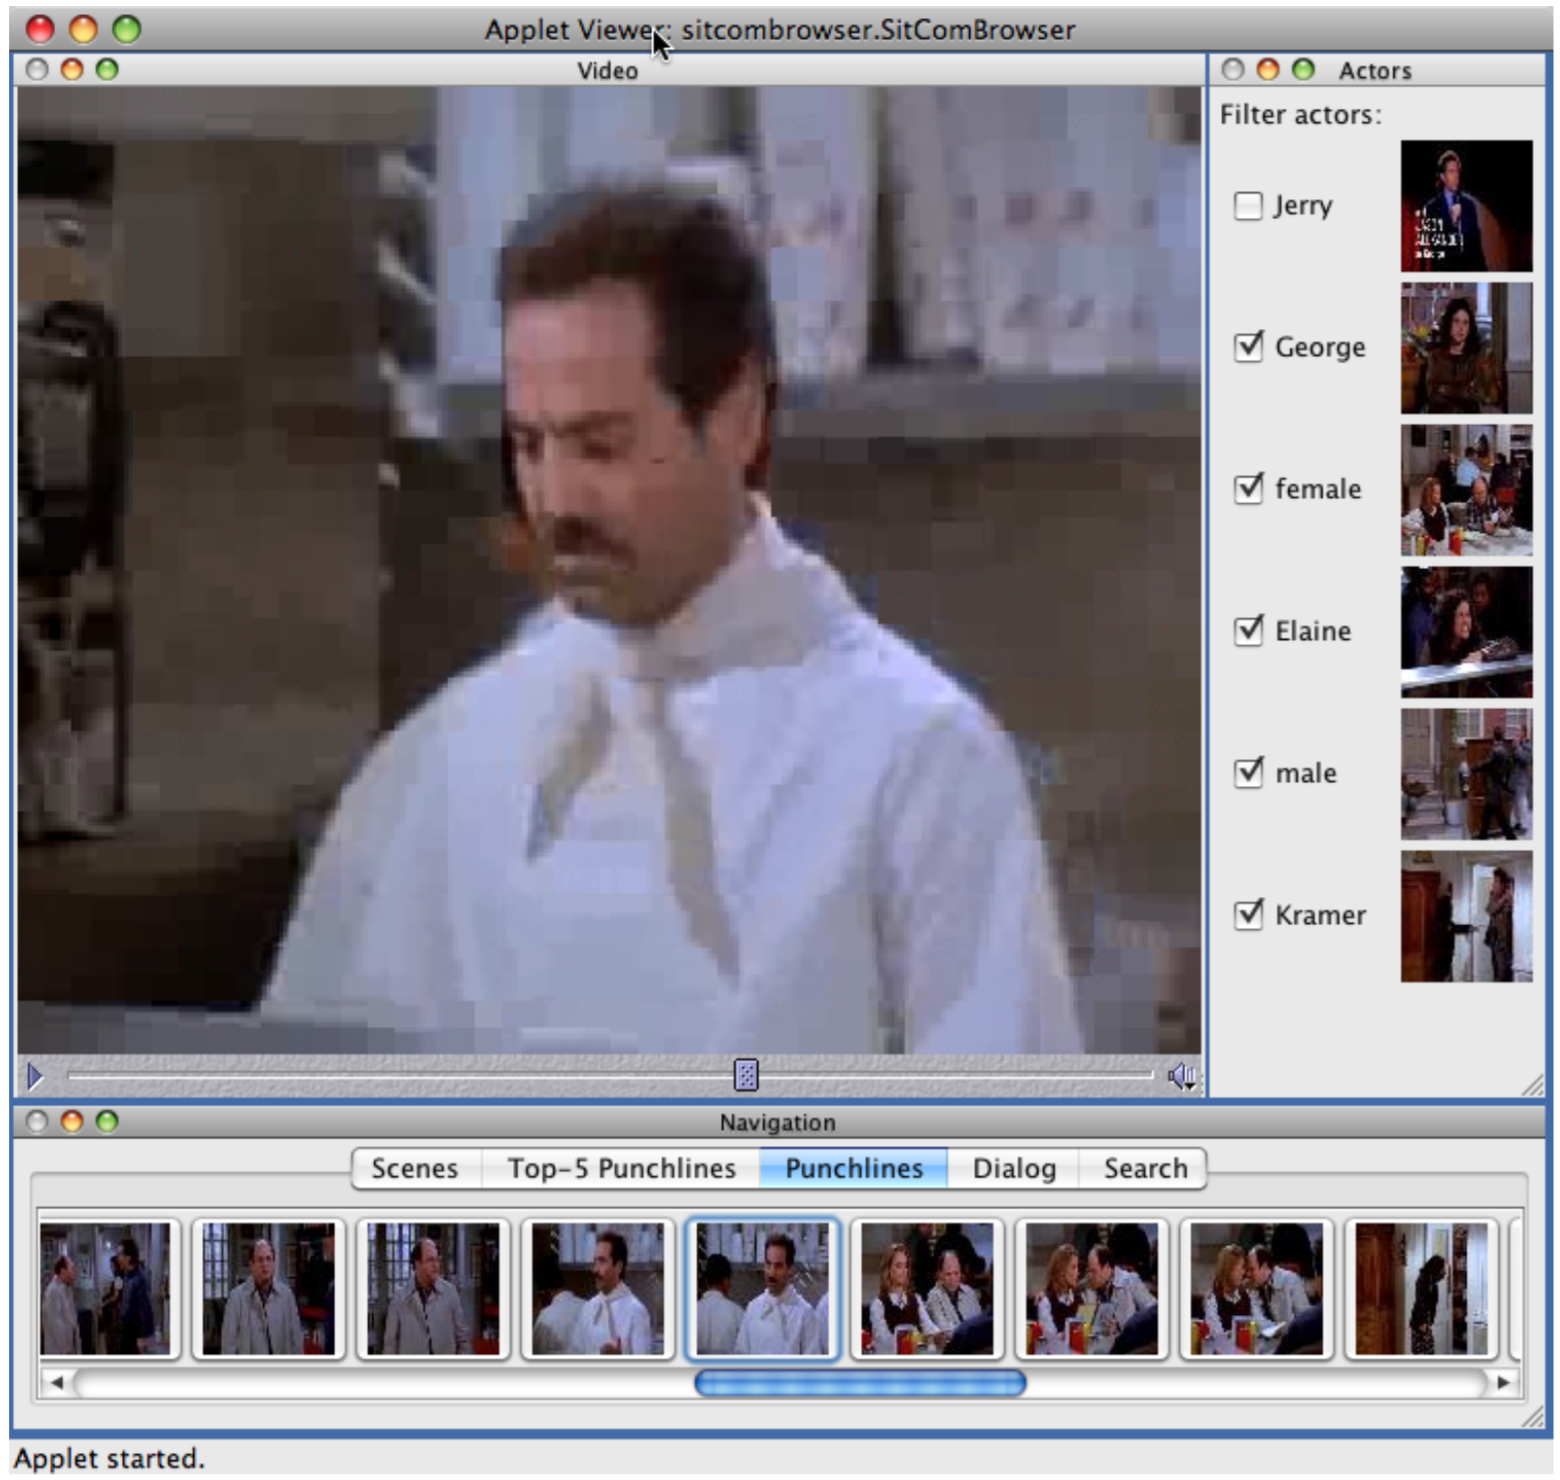
\includegraphics[scale=0.4]{./images/39.png}
\caption{Joke-O-Mat Benutzeroberfläche \cite{friedland2009joke}}
\label{jokeomat}
\end{center}
\end{figure}
Die Audioanalyse ist so entwickelt worden, dass auch das Lachen der Zuschauer in der Serie erkannt wird. Davon ausgegangen, dass nach einem Satz eines Darstellers, gefolgt von Gelächter, ein Witz gemacht wurde, konnten diese Szenen auch als solche markiert werden. Der Nutzer kann damit ebenfalls von einem Witz zum nächsten springen. Der Joke-P-Mat wurde speziell am Beispiel der Serie Seinfeld entwickelt, was auch aus der Benutzeroberfläche ersichtlich ist. In der rechten Spalte können alle Schauspieler selektiert werden, nach denen gesucht werden soll, sowie eine geschlechtsspezifische Suche. In der unteren Navigationsspalte gibt es verschiedene Menüs, die beispeilsweise eine Übersicht über alle Witze gibt. Mit einem Klick auf einen Bildausschnitt gelangt der Nutzer direkt in diese Szene. Mit einer gewöhnlichen Navigationsleiste, sowie einem Knopf zum Abspielen, bzw. Pausieren ist man jederzeit in der Lage, manuell zu navigieren.
Der Joke-O-Mat zeigt sehr gut, dass Videonavigation nicht nur auf Grundlage des visuellen Teils gemacht werden kann, sondern auch andere Komponenten eines Multimediums mit einbezogen werden können.

Im nächsten Kapitel werden Alternativen zur Inhaltsanalyse vorgestellt, und zwar die Möglichkeit durch Veränderung der Visualisierung des Inhaltes und erweiterter Navigation ebenso die Durchsuchbarkeit zu vereinfachen und beschleunigen.

\subsection{Alternative Inhaltsvisualisierung und Navigation}

Bisher bieten nur wenige Videoplayer eine Alternative zur klassischen Navigationsleiste. Wie im Kapitel zur klassischen Navigation schon gezeigt wurde, hat der YouTube Player ein kleines Vorschaufenster, welches anzeigt, wo man im Video hinspringen wird. Neben der algorithmischen Analyse von Videos ist oftmals eine andersartige Darstellung des Inhalts und auch Navigation vollkommen ausreichend, um dem Nutzer einen Vorteil zu verschaffen. Vor allem wenn der Nutzer keine geeignete Suchanfrage machen kann, da er nicht weiß, wie man das zu Suchende beschreiben soll \cite{muller2012demonstration}. Ein besonderes Kriterium für Massentauglichkeit ist eine einfache Handhabung des Tools. Zu flache Lernkurven können den Nutzer frustrieren und zum Aufgeben bewegen. Es gibt einige Versuche dieses Dilemma zu bewältigen, von denen im Folgenden einige vorgestellt werden. \cite{schoeffmann2014video}

Der \emph{Baum-basierte Video Browser} von del Fabro erlaubt es innerhalb kürzester Zeit sich einen Überblick über den Inhalt eines Videos oder Videobibliothek zu verschaffen. Am Beispiel eines einzelnen Videos wird nach dem Öffnen eine Übersicht von Vorschaubildern angezeigt, die jeweils alle eine identisch lange Zeitspanne abbilden. Die Anzahl an Vorschaubildern ist frei konfigurierbar, sodass man beispielsweise eine 3 mal 3 Zellen Übersicht einstellen kann. Bei einem Video mit 90 Minuten Länge steht jedes der Bilder also für 10 Minuten des Videos. Mit einem Klick auf eines der Bilder gelangt man eine Stufe tiefer in der Hierarchie, wodurch nun wieder 9 Vorschaubilder angezeigt werden, die den Inhalt repräsentieren, welcher von dem ausgewählten Bild abgedeckt wurde. In dieser Hierarchieebene werden also diese 10 Minuten wieder aufgeteilt, sodass jedes Bild etwas über eine Minuten des Videoinhalts anzeigen. Abbildung 3.4 zeigt wie sich der Baum verzweigt und so der Inhalt des Videos sichtbar wird.
\begin{figure}[h]
\begin{center}
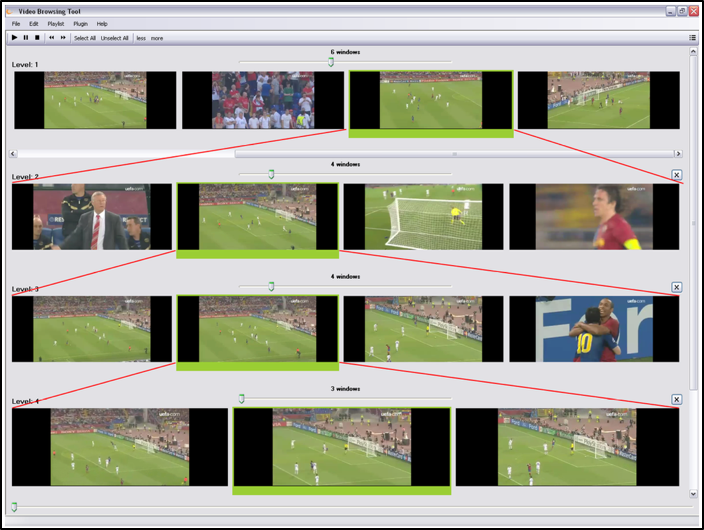
\includegraphics[scale=1.1]{./images/8.png}
\caption{Hierarchische Baumübersicht \cite{del2010instant}}
\label{baum_browser}
\end{center}
\end{figure}
Das besondere ist noch, dass der Nutzer mit Hilfe von Schiebereglern durch alle sichtbaren Einzelsequenzen durchnavigieren kann und so die zu suchende Stelle schnell auffindbar machen kann. Die Audiospur ist nur in der Einzelübersicht aktiviert, da beim Abspielen von mehreren Tonspuren gleichzeitig ein schlechtes Benutzererlebnis entsteht. Der Videoplayer wurde so implementiert, dass eine Anbindung an ein Inhaltsanalysetool möglich ist. \cite{del2010instant}

Der\emph{ 3D Video Browser} von Müller, Schmole und Schöffmann kombiniert eine 3-dimensionale Darstellung des Inhalts mit einer interaktiven und animierten Navigation. Ähnlich wie der Baum-basierte Videobrowser von del Fabro ist hier der Ansatz das Video oder die Videosammlung hierarchisch darzustellen. Durch die 3-dimensionale Anordnung lassen sich die verschiedenen Ebenen aber beliebig im Raum verteilen. Ansätze von 3D-Darstellungen gab es schon zuvor, jedoch unterstützten diese keine hierarchische Navigation, sondern waren allein auf die Darstellung der Navigationsleiste beschränkt \cite{divakaran2005augmenting}. Beim 3D Videobrowser hat der Nutzer zudem die Möglichkeit zwischen 8 verschiedenen Darstellungsoptionen zu wählen. Mit einem Klick auf ein Segment wird die Szene abgespielt. Innerhalb der Anordnung kann man sich zudem völlig frei im Raum bewegen und den gesamten Inhalt erkunden. Der 3D Videobrowser ist auch in der Lage eine komplette Videobibliothek in dieser Form abzubilden und navigierbar zu machen. \cite{muller2012demonstration}

Ein dritter Videobrowser, welcher den Inhalt an sich nicht verändert darstellt, sondern nur eine erweiterte Navigationsleiste implementiert, ist der \emph{ZoomSlider} von Hürst und Jarvers. Der Grundgedanke ist, dass bei sehr langen Videos eine Navigation mit herkömmlicher Suchleiste oft unpräzise ist da beim Bewegen des Schiebereglers die Sprünge zwischen den einzelnen Sequenzen zu groß sind und der Inhalt dadurch nicht erfasst wird. Um dieses Problem zu beheben kann man während dem Anschauen des Videos das Mausrad vertikal drehen, um in die teilbasierte Navigationsleiste hereinzuzoomen. Dadurch wird der Bewegungsradius eingeschränkt und der Nutzer kann verfeinert den Inhalt erkunden und weniger Stellen werden übersprungen. Durch das nach unten drehen des Mausrades wird der Balken wieder hochskaliert, sodass die ursprüngliche Navigation wieder möglich ist. Die Benutzeroberfläche gibt während der Bedienung Rückmeldung und zeigt an, wie stark man in die Suchleiste hereingezoomt hat. Ein besonderer Vorteil dieser Navigationsmethode ist, dass große Videodateien genauer untersucht werden können, ohne den Vollbildmodus zu verlassen. \cite{hurst2005interactive}

Azzopardi et al. \cite{azzopardi2012yoosee} haben einen Videobrowser entwicklet, der sich aufgrund der Einfachheit in der Bedienung speziell an Kleinkinder im Alter zwischen zwei und sechs Jahren richtet. Die Benutzeroberfläche ist ähnlich wie ein Karussell aufgebaut. Die folgende Abbildung 3.6 gibt eine Übersicht über den sogenannten \emph{YooSee} Browser.
\begin{figure}[h]
\begin{center}
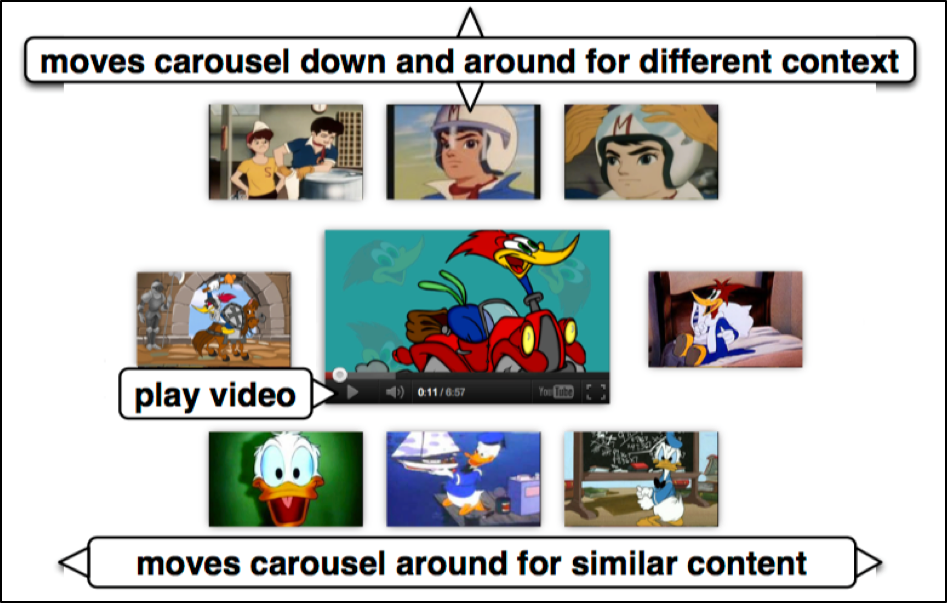
\includegraphics[scale=0.9]{./images/40.png}
\caption{YooSee Benutzeroberfläche \cite{azzopardi2012yoosee}}
\label{yoosee}
\end{center}
\end{figure}
Jede der drei sichtbaren Reihen entspricht einer Kategorie, die in einer Administrationsoberfläche zuvor festgelegt werden müssen. Diese sind vergleichbar mit einer Wiedergabeliste. Das mittlere Video ist dieses, welches gerade abgespielt wird. Mit einem Klick auf das Vorschaubild rechts bzw. links daneben, wird ein Video zum gleichen Kontext abgespielt. Um zu einer anderen Kategorie zu wechseln, kann das Kind auf die obere oder untere Reihe klicken. Da der Videobrowser zum Abspielen Youtube Videos verwendet, wird auch der Standardyoutubeplayer für eine Navigation innerhalb eines Videos benutzt.

Da es sehr aufwändig ist solche Videobrowser einheitlich zu evaluieren, wurden verschiedene Wettbewerbe ins Leben gerufen. Das folgende Kapitel zeigt die zwei wichtigsten Wettbewerbe, die sich in dieser Thematik spezialisiert haben.

\section{Videobrowser Evaluierung}

Benutzerstudien eignen sich sehr gut, um neue Ideen realitätsnah zu untersuchen, jedoch lassen sich verschiedene Videoplayer nur sehr schwer direkt miteinander vergleichen. Unterschiedliche Bedingungen wie das verwendete Videomaterial, andere Fokusse und Testkandidaten sind hierfür nur wenige Gründe. Im Rahmen von Wettbewerben wird den Forschern die Möglichkeit geboten ihre Videobrowser in einer einheitlichen Umgebung gegeneinander antreten zu lassen und so die Leistungsfähigkeit komparabel zu messen. In diesem Kapitel werden die zwei bekanntesten dieser Art vorgestellt und zwar der \emph{Video Browser Showdown} und \emph{TREC Video Retrieval Evaluation}.

\subsection{Video Browser Showdown}

Um die Forschung in Bereich der Videoplayer für Videosuche, Navigation, Interaktion und Darstellung weiter voranzutreiben, wurde im Jahr 2012 der erste Video Browser Showdown als Sonderveranstaltung der International MultiMedia Modeling Conference ins Leben gerufen. Vor allem sollen Methoden und Ideen umgesetzt werden, die sich auf den Nutzer orientieren. Die Veranstaltung findet seither auf jährlicher Basis statt. Im Allgemeinen sehen die Aufgaben so aus, dass die Teilnehmer eine Reihe von Ausschnitten gezeigt bekommen, welche sie in einem längeren Video, oder auch in einer Videosammlung finden müssen. Da der Fokus des Wettbewerbs vor allem darin liegt die Nutzerinteraktion zu fördern, sind automatischen Suchaufgaben, wie beispielsweise eine Textsuche, nicht erlaubt. Vielmehr geht es darum, durch alternative Navigation und filtern des Inhaltes, die gesuchte Stelle so schnell wie möglich zu finden. Da alle Teilnehmer alle Aufgaben erledigen müssen, lassen sich so die Stärken und Schwächen herauskristallisieren. Die Videos sind beim Video Browser Showdown aus verschiedenen Arten ausgewählt worden, sodass kein Videoplayer mit einem Vorteil ins Rennen geht. So gibt es schwarz-weiß Aufnahmen, welche mit viel und welche mit wenig Bewegung. Die gezeigten Ausschnitte haben eine länge von 20 Sekunden, welche jeweils aus einem in etwa einstündigen Video extrahiert wurden. Dazu zählen die Aufgaben zur Kategorie KIS, also Know-Item-Search, denn die Teilnehmer wissen wie das zu suchende Objekt aussieht, wissen aber nicht wo es zu finden ist. Alle Tools sind an den VBS Server angeschlossen, welcher die Zeit misst, bis eine Lösung abgegeben wird. Dazu kommen noch sogenannte Penalties, also Strafzeit, die bei dem Abgeben einer falschen Lösung verteilt werden. Die Zeiten werden auf Punkte pro Aufgabe umgeschichtet, woraus sich schließlich am Ende durch Addition eine Gesamtpunktzahl ergibt. Mit dieser wird dann der Gewinner ermittelt. Da die Entwickler der Videobrowser selbst Experten sind, was deren Bedienung angeht, werden insgesamt zwei Durchläufe gemacht. Die erste Runde ist die sogenannte Expertenrunde, bei denen die Entwickler selbst die Aufgaben durchführen. Die zweite Runde, die Novice Runde, bei der zufällig ausgewählte Teilnehmer der Konferenz die Bedienung übernehmen, welche alle Experten im Bereich von Multimedia sind. In den ersten beiden Jahren war der VBS auf eine Stunde begrenzt, aber durch den hohen Bedarf mehr Daten und Erkenntnisse zu sammeln, wurde im Jahr 2014 die Dauer auf 5 Stunden ausgedehnt. Dadurch konnten viel mehr Aufgaben durchgeführt werden, denn pro Aufgabe wird ein 3-minütiges Zeitfenster gegeben. Viele verschiedene Systeme wurden mittlerweile seit 2012 präsentiert, wobei sich herausgestellt hat, dass nicht immer das System gewonnen hat das viele verschiedene Analysemethoden implementiert hatte, sondern eine einfache und schnelle Navigation und auch Darstellung des Videoinhalts ebenso einen mindestens genau so großen Einfluss hat. \cite{schoeffmann2014video} \cite{schoeffmann2014user}

\subsection{TREC Video Retrieval Evaluation}

Die TREC Video Retrieval Evaluation, kurz TRECVID, wurde im Jahr 2001 von der Disruptive Technology Office (DTO) und dem National Institute of Standards and Technology (NIST) ins Leben gerufen. Des Weiteren erhält die Konferenz Unterstützung von verschiedenen Instituten der US Regierung. Die Ziele der TRECVID Konferenz sind die Forschung im Bereich der Informationsgewinnung auf Basis von besonders großen Video Sammlungen zu fördern, sowie die Kommunikation zwischen Wissenschaft, Industrie und der Regierung zu steigern. Dabei sollten Ideen ausgetauscht werden, um den Fortschritt weiter zu unterstützen. Durch den Austausch von Ideen sollen die Technologien eine weitere Verbreitung und Anklang in der Gesellschaft finden, welche letztendlich dabei helfen sollen, die Probleme aus der realen Welt zu lösen. Im Gegensatz zum Video Browser Showdown liegt hier der Fokus hier nicht nur auf der Endnutzerbedienbarkeit, sondern zudem auf der Effektivität von Systemen, die alleine mit automatischer Inhaltsanalyse arbeiten. Denn es gibt neben den KIS Ausgaben, auch Aufgaben aus den Bereichen der vollkommen automatischen Suche. Hierbei werden großen Mengen an Multimediadateien verarbeitet, um bestimmte Ereignisse zu finden. Insbesondere bei bei Überwachungsvideos sollten Objekte automatisch erkannt werden und eine Liste mit gefundenen Szenen als Ergebnis geliefert werden. Ein Indikator, welcher für eine Messung herangezogen wird, ist die Genauigkeit dieser Ergebnisse. Um die Resultate dieser umfangreichen Evaluierung so repräsentativ wie möglich zu machen, wird immer viele Stunden Videomaterial herangezogen. Im Jahr 2010 waren es beispielsweise 400 Videostunden \cite{over2005trecvid} \cite{over2011trecvid}. Da mehrere Kategorien bzw. Tracks existieren, muss nicht jedes Team bei jeder Art Aufgabe teilnehmen. Wie zuvor schon erwähnt können die Aufgaben in insgesamt drei verschiedene Aufgabenbereiche aufgeteilt werden. Im einzelnen sind das Suchaufgaben, bei denen die Systeme vollständig automatisch arbeiten, also keine menschliche Interaktion bei der Suche notwendig ist. Die zweite Art von Aufgaben sind manuelle Suchaufgaben, bei denen eine Person die Suchanfrage selbst formuliert und diese dem System als Parameter übergibt. Die dritte Kategorie sind interaktive Suchen, bei denen der manuelle Ansatz insofern erweitert wird, dass die gelieferten Ergebnisse vom Nutzer evaluiert werden und die Suchanfrage angepasst werden kann, sodass die neuen Ergebnisse genauer sind. Objekte, nach denen gesucht werden kann, können von ganz unterschiedlicher Natur sein. Beispielsweise kann nach ganz allgemeinen Eigenschaften gesucht werden, wie Bewegungen oder Farben. Dies kann jedoch auch expliziter sein, wie die Suche nach Gesichtern, Logos oder Texturen. Die Evaluierung der teilnehmenden Video Analyse Systemen erfolgt vollständig auf Basis deren gelieferten Ergebnisse, welche in einen einheitlichen Format sein müssen. Diese Ergebnisse werden dann abhängig vom Typ der Suchaufgabe entweder manuell bewertet oder von einem automatischen Bewertungssystem. \cite{niaz2014eurecom}

In diesem Kapitel wurden verschiedene Methoden und Applikationen von Videobrowsing vorgestellt, sowie Möglichkeiten für deren Evaluierung. Im folgenden Kapitel wird erörtert, wie solche Systeme auf mobilen Geräten umgesetzt werden und welche Anforderung es dabei gibt.

\chapter{Videonavigation auf Tablets und Smartphones}

In den vorherigen Kapiteln wurden insbesondere Browser vorgestellt, die mit einem Desktop Computer oder Laptop zu bedienen waren. Wenn es aber zum Thema Smartphones und Tablets kommt, kommen weitere Faktoren hinzu, die die Probleme noch verstärken. Aufgrund limitierter Bildschirmgröße müssen Kompromisse bei der Darstellung eingegangen werden, denn den Inhalt einfach zu verkleinern ist in vielen Fällen unmöglich. Die Interaktion muss für mobile Geräten mit Touch-Eingabe ebenso komplett überdacht werden, da Eingabeperipherie wie Maus und Tastatur nicht zur Verfügung stehen. Da aber heutzutage die Touchscreens mit einer hohen Präzision arbeiten, bieten sich somit ganz neue Möglichkeiten, was das Bedienkonzept betrifft. In diese Richtung weiter zu entwickeln erhält einen besonderen Stellenwert, da mittlerweile eine Vielzahl von verschiedenen Medien mobil konsumiert werden. Darunter sind beispielsweise Fernsehsendung, die in Echtzeit übertragen werden können, Filme und Serien, aber noch viel wichtiger ist die private Videosammlung. Hierbei zählen Videos, die der Nutzer selbst aufgenommen hat, sowie Videomaterial, dass direkt aus dem Internet auf das Gerät geladen wurde. Durch die Vielfalt ergibt dich auch, dass die Videodateien sich in ihren Eigenschaften stark unterscheiden. So sind die Aufnahmen von hoher bis niedriger Qualität, die Länge der Aufnahmen schwankt stark und auch die Aufnahmen werde sehr amateurhaft bis hochprofessionell produziert. Dies zusammen macht es umso schwieriger einen Videoplayer vorzuschlagen, welcher mit allen Arten sinnvoll zu bedienen ist. Ein weiteres Problem sind die teilweise stark eingeschränkten Ressourcen. Im Vergleich zu einem vollwertigen Heimcomputer, welcher in der Regel mit viel leistungsfähigeren Prozessoren und mehrere Gigabyte Arbeitsspeicher ausgestattet ist, können bei Smartphones und Tablets nur stromsparende Komponenten verbaut werden, um eine höher Akkulaufzeit zu erreichen und die Hitzeentwicklung zu minimieren. \cite{hurst2007interactive}

Im folgenden Kapitel werden die Besonderheiten aufgearbeitet, die es bei mobilen Geräten bezüglich Videobrowsing gibt und welche Faktoren bei der Gestaltung von mobilen Applikationen beachtet werden sollten. Des Weiteren werden Lösungsvorschläge präsentiert, die als Motivation dienten, für die Implementierung des Prototyps, der im Rahmen dieser Arbeit entwickelt und evaluiert wurde.


\section{Interface Design Guidelines}

In den vorherigen Kapiteln wurde schon angeschnitten, das für mobile Geräte andere Design Regeln bezüglich deren Benutzeroberfläche und Interaktionsmöglichkeiten gelten. Im Jahr 2004, also noch bevor Smartphones und Tablets eine derart weitreichende Verbreitung erlangt haben, haben Gong und Tarasewich diese Probleme genauer untersucht und einen Design-Guide veröffentlicht. Dabei haben sie versucht die sogenannten „Golden Rules of Interface Design“ von Shneidermann, welche im Jahr 1992 für Desktop Computer entwickelt wurden, auf mobile Geräte zu übertragen \cite{shneiderman1992designing}. Diese insgesamt 8 Regeln wurden um weitere 7 Regeln erweitert. Eine dieser Regeln ist, dass das Design ganz allgemein für kleine Bildschirme angepasst werden muss. Hierbei sollen beispielsweise Texte aus einer vorgefertigten Menge auswählbar sein, anstatt eine manuelle Texteingabe zu erfordern. Haptische Rückmeldung vom System sollten ebenso Teil der Software sein. Was ebenso beachtet werden sollte ist, dass die Interaktion so einfach muss wie möglich, da komplizierte Aufgaben den Nutzern vom eigentlichen Inhalt ablenken. Am Beispiel eines Videoplayers kann eine besonders aufwändige Navigationsmethode den Nutzer derart fordern, dass dieser vom Video nur wenig aufnimmt und so das Ziel leicht verfehlt werden kann. Ein weiterer Punkt ist der, dass die Informationen, die die Applikation bereitstellt, limitiert werden müssen, sodass der Nutzer auch hier nicht überfordert wird. Das bedeutet im Detail, dass am Beispiel des Videoplayers nur relevante Informationen, wie die aktuelle Position oder sonstige Inhalte, die für die explizite Interaktion notwendig sind, angezeigt werden sollten. Einer der wichtigsten Punkte ist jedoch, dass die Benutzeroberfläche von Grund auf Ansprechend gestaltet werden muss, unabhängig von Zweck der Applikation. \cite{gong2004guidelines}

\section{Multi-Touch Bildschirme und Gesten}

Berührungsempfindliche Bildschirme ermöglichen eine besonders einfache Kommunikation mit einem Computer. Die direkte Interaktion ist für die meisten Nutzer, insbesondere Anfängern sehr ansprechend, da man nicht erst den Umgang mit einer Eingabeperipherie üben muss. Daraus ergibt sich eine steile Lernkurve. Problematisch wird es nur, wenn der Nutzer eine Benutzeroberfläche bedienen muss, die eigentlich für den Gebrauch mit einer Maus und Tastatur entwickelt wurde. Aktionen wie ein Rechts-Klick werden hier zu einem großen Hindernis. Auch die Größe der Knöpfe spielen hier eine nicht unwesentliche Rolle bezüglich des Komforts \cite{benko2006precise}. Anfangs war dies auch kein großes Problem, da Geräte mit Touchscreens in der Regel nicht in privaten Haushalten zu finden waren. Vor allem Bankautomaten, Zugticketautomaten und Informationskiosk setzten auf dieses Konzept. Dadurch wurde die Langlebigkeit dieser Maschinen erheblich verbessert, denn auf beweglichen Teile wie Mäuse konnte verzichtet werden \cite{albinsson2003high}. Generell gibt es berührungsempfindliche Bildschirme schon seit Jahrzenten, jedoch haben sie erst durch das Apple iPhone derart an Popularität gewonnen. Die Steuerung ist enorm präzise, weshalb die Applikationen keinerlei Hardware-Knöpfe mehr benötigen. Virtuelle Tastaturen und schnell durchsuchbare Listen wurden damit massentauglich. Multi-touch gibt den Bildschirmen die Fähigkeit auf Eingaben zu reagieren, die mit mehr aus nur einen Finger gemacht werden. Viele Gesten wurden somit erst möglich, die heutzutage allgegenwärtig sind. Diese sind beispielsweise Wischgesten, Pinch-Gesten, die beim vergrößern bzw. verkleinern von Objekten zum Einsatz kommen, sowie Rotationsgesten, um Fotos zu drehen. Die Objekte können daher direkt manipuliert werden, ohne dass der Nutzer sind Eingabebefehle wie Tastenkombinationen merken muss \cite{kane2008slide}. Die weitverbreitetste Technologie, die bei den heutigen Smartphones und Tablets zum Einsatz kommen, sind sogenannte kapazitive Touchscreens, die mit Hilfe von elektrischer Spannung auf dem Glas, die durch die Finger unterbrochen wird, die exakte Position feststellen können. \cite{laufs2013aufbau} Generell gibt es heutzutage sehr viele verschiedene Wischgesten, um in einem mobilen Betriebssystem oder auch einer einzelnen Applikation zu navigieren. Alleine Apple stellt insgesamt sechs zweidimensionale Standardgesten den Entwicklern in einer Programmierschnittstelle zur Verfügung. Dazu zählen beispielsweise die schon genannten Pinch- und Rotationsgesten. In der folgenden Abbildung 4.1 sind alle Gesten einzeln dargestellt.\begin{figure}[h]
\begin{center}
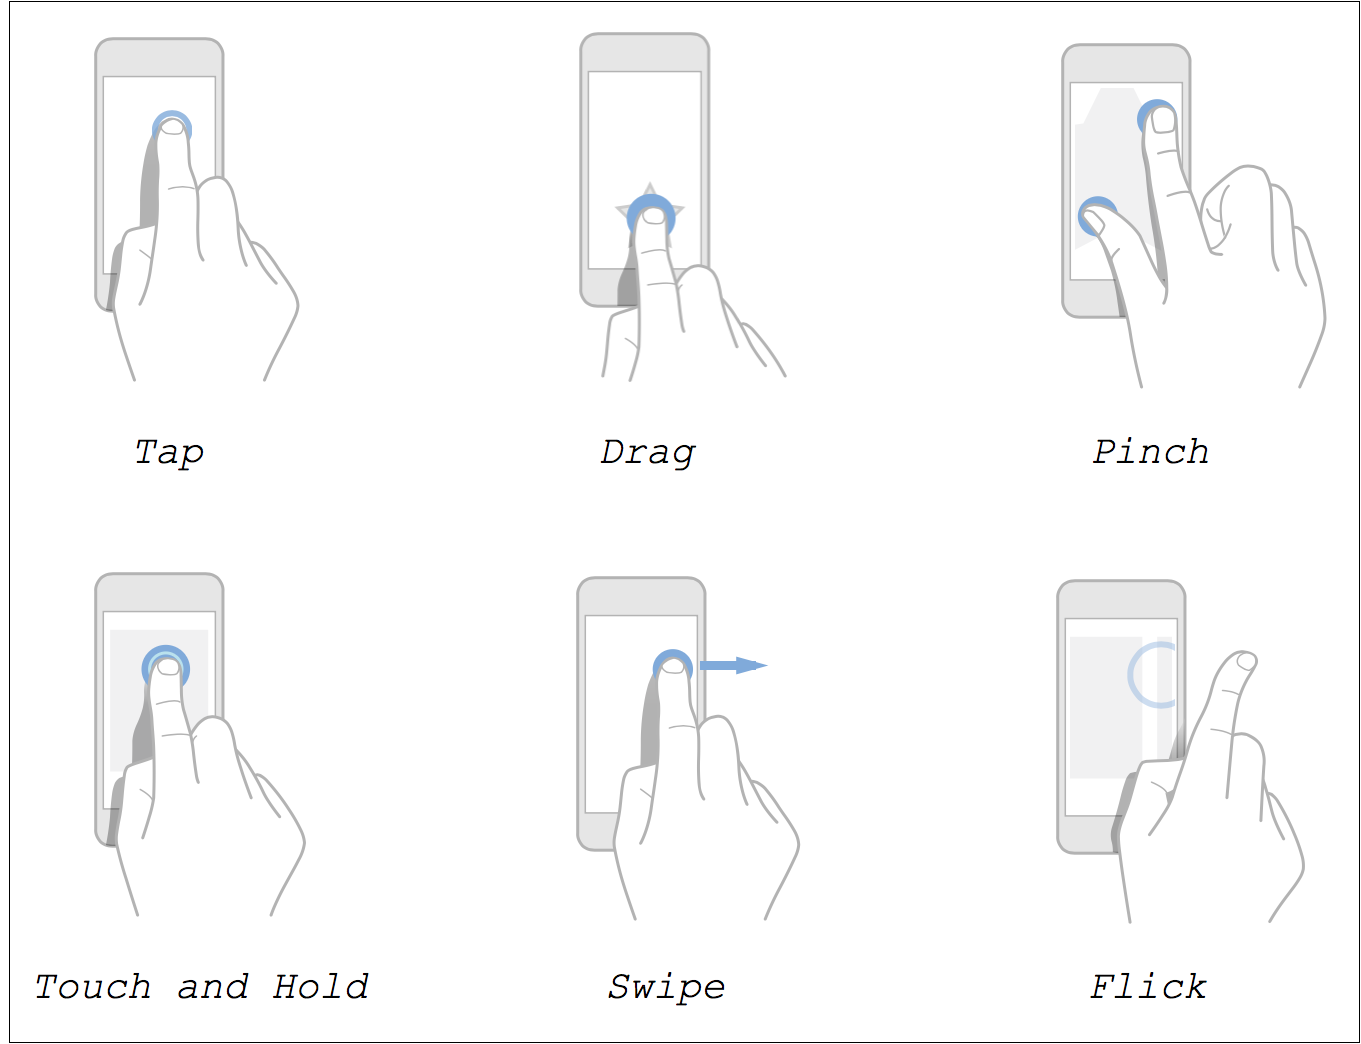
\includegraphics[scale=0.31]{./images/42.png}
\caption{Standardgesten für iOS \cite{appleGesturesStandard}}
\label{applegesten}
\end{center}
\end{figure}Bis auf die Pinch-Geste sind alle Gesten mit einem Finger durchzuführen, jedoch kann dies so angepasst werden, dass eine Geste mehrere Finger benötigt. Beispielsweise ist die Rotationsgeste eine Drag-Geste, die mit zwei Finger gemacht wird. Um Objekte anzutippen kann eine einfach Tap-Geste benutzt werden, die auch mit so eingestellt werden kann, dass zwei oder öfters getippt werden muss. Dies ist beispielsweise der Fall, wenn man einen Text auf einer Internetseite vergrößern und zentrieren möchte. Die Touch-and-Hold-Geste kann mit dem Rechtsklick auf einem Desktop-Computer verglichen werden. Der Nutzer berührt ein Element auf dem Bildschirm und bleibt so lange mit dem Finger auf dem Bildschirm, bis sich ein Kontextmenü öffnet. Dies kann beispielsweise benutzt werden, um einen Text zu markieren. Zwei Gesten, die sich sehr ähnlich, jedoch nicht das gleiche sind, ist die Swipe-Geste und die Flick-Geste. Die Swipe-Geste wird in der Regel verwendet, wenn eine genauere und kontrollierte Navigationsinteraktionen gemacht werden müssen. Dies ist zum Beispiel der Fall, wenn man innerhalb einer Liste eine Zelle seitlich mit einem Wisch verschiebt, sodass eine Löschfunktion zum Vorschein kommt. Ein weiterer Anwendungsfall ist das Betrachten einer Reihe von Fotos, bei den man mit einem horizontalen Wisch von einem Foto zum nächsten gelangt. Die Flick-Geste hingegen wird meist schneller und unpräziser durchgeführt. Mit einer ruckartigen Bewegung kann eine Beschleunigung einer Liste gestartet werden, bei der man nicht genau vorhersehen kann, an welcher Stelle man sich befinden wird, wenn die Bewegung von alleine zum Stillstand gekommen ist. Aus diesem Grund können solche Interaktionen mit einer Tap-Geste unterbrochen werden, sodass das durchblättern der Liste gestoppt wird. \cite{appleGesturesStandard}

Der Prototyp des Videoplayers, der im Rahmen dieser Arbeit entwickelt wurde, basiert auf einer Flick-Gesten Navigation. In den folgenden Kapiteln werden jedoch zuerst anderen Arten der Videonavigation auf mobilen Geräten aufgearbeitet.

\section{Standardvideoplayer}

Jedes Smartphone und Tablet kommt mit einem vorinstallierten Standardvideoplayer beim Kunden an. Diese unterscheiden sich im Kontext von Bedienung und Benutzeroberfläche in der Regel kaum voneinander. Üblicherweise weißt die Oberfläche einen Start-Knopf, bzw. Pause-Knopf, der sich je nach Wiedergabestatus verändert, zwei Knöpfe um jeweils in die vorherige, bzw. nächste Datei zu wechseln und einen Lautstärkeregler. Um aber innerhalb eines Videos zu navigieren wird eine Suchleiste angezeigt, die je nach zeitlicher Position in Relation zum Video einen Punkt markiert, welcher sich auch verschieben lässt. Im Falle des Standardplayers der iOS Geräte iPhone, iPod und iPad kann der Nutzer bei gedrückt halten des Zeigers und vertikalem Wisch nach unten die Bewegung verlangsamen, sodass der Vorlauf, bzw. Rücklauf verfeinert ist. Die Position an der Oberseite des Bildschirmes ist aber aus benutzertechnischer Sicht nicht optimal, da der Inhalt mit der Hand verdeckt wird \cite{huber2010toward}. Der VLC Videoplayer von VideoLAN ist stark an das Bedienkonzept des Standardplayers anlehnt.
\begin{figure}[h]
\begin{center}
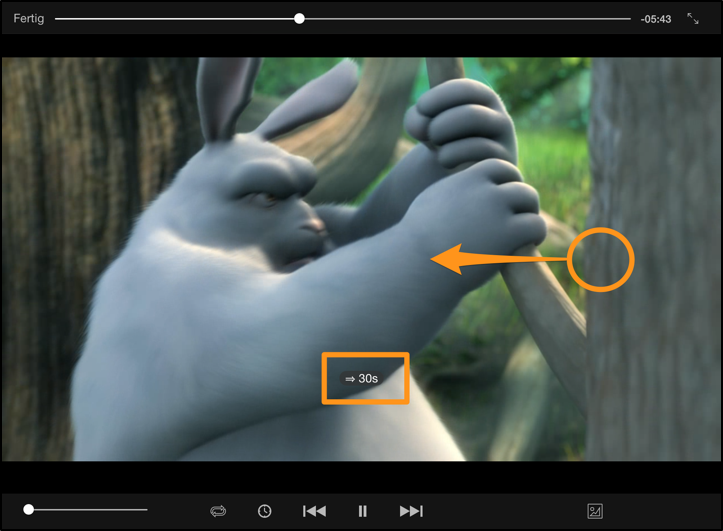
\includegraphics[scale=1.0]{./images/9.png}
\caption{VLC Player auf einem iPad}
\label{vlc_ipad}
\end{center}
\end{figure}Die folgende Abbildung 3.5 zeigt den Videoplayer auf einem iPad mit 9,7“ Bildschirm. Das Besondere an dieser Applikation ist jedoch nicht das Bedienkonzept. Der VLC Player Legt den Fokus auf eine hohe Kompatibilität zu einer Vielzahl von Audio und Video Formaten. Dennoch versuchen solche standardisierten Videoplayer mit Hilfe von extra Funktionen die Navigation etwas zu vereinfachen und sich differenzieren. Es gibt unterschiedliche Ansätze Wischgesten für die Navigation innerhalb eines Videos oder einer Videobibliothek zu verwenden. Häufig werden Methoden verwendet um mit einer horizontalen Wischbewegen im Video entweder nach vorne oder nach hinten zu springen. Dadurch verliert der Benutzer offensichtlich Informationen darüber, was zwischen den beiden Szenen passiert. Insbesondere wenn das Ziel ist den gesamten Inhalt eines Videos zu erfassen, ohne sich den Inhalt in Standardabspielrate anzusehen, kommen aktuelle Videoplayer an ihre Grenzen. Als Beispiel einfacher Wischfunktionen ist der VLC-Player für iOS in der Version 2.6.6. Mit einem horizontalen Wisch von rechts nach links springt der Benutzer um fixe 30 Sekunden nach vorne im Video. Problematisch hierbei ist, dass der Benutzer keine Möglichkeit hat das Intervall anzupassen, um sich ggf. schneller bzw. langsamer im Video zu bewegen. Des Weiteren ist die fixe Sprunglänge suboptimal für besonders lange oder kurze Videos. \cite{VideoLANVLCPlayerforiOS}

Im folgenden Kapitel werden Prototypen und Konzepte von Videobrowsern vorgestellt, die sich als Alternative zu klassischen Videoplayern positionieren und für den Einsatz auf mobilen Geräten bezüglich Bedienung und Darstellung optimiert sind.

\section{Videobrowsing auf mobilen Geräten}

Dieses Kapitel widmet sich den Videobrowsern, die speziell für mobile Geräten mit Touch-Eingabe optimiert sind. Der Fokus liegt hier insbesondere auf die Player, die den entweder den Inhalt alternativ darstellen oder in punkto Navigation sich von dem klassischen Suchleistenprinzip abwenden.

Der ThumbBrowser von Hudelist, Schöffmann und Böszoermenyi ist ein Videoplayer, der sich die natürliche Haltung des Tablets im Querformat in zwei Händen zum Vorteil macht, da dann die beiden Daumen des Nutzers frei beweglich sind. Das Querformat wird von den Nutzern besonders häufig gewählt, da bedingt durch die Aufnahme der Inhalt des Videos so den Bildschirmplatz am besten ausnutzt. Insgesamt enthält der ThumbBrowser zwei Menüs, die jeweils von einem Daumen gesteuert werden. In Abbildung 3.6 ist die Benutzeroberfläche zu sehen, wie sie von einer Person bedient wird.
\begin{figure}[h]
\begin{center}
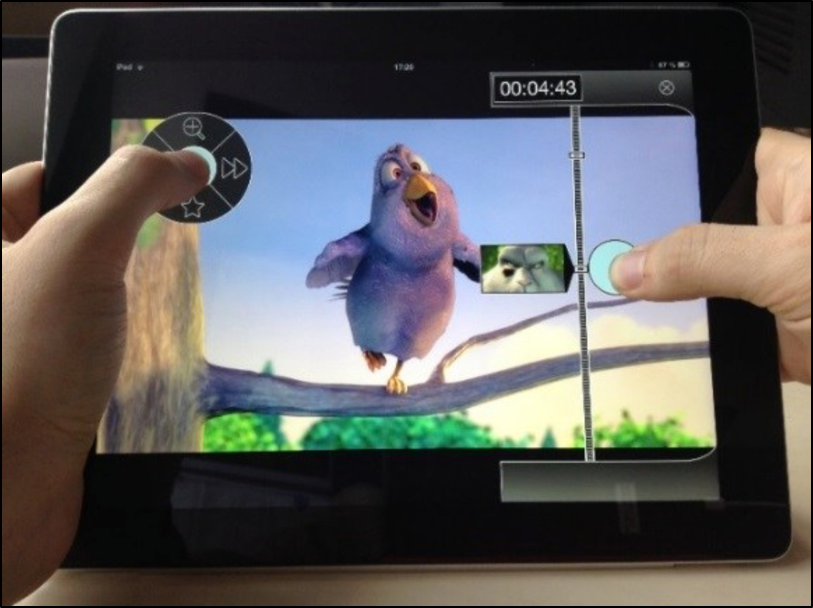
\includegraphics[scale=1]{./images/10.png}
\caption{ThumbBrowser in Benutzung \cite{hudelist2013mobile}}
\label{thumbbrowser}
\end{center}
\end{figure}
Die beiden Menüs sind nur sichtbar, wenn der Bildschirm berührt wird. Des Weiteren positionieren sie sich immer an der Stelle, an welcher man mit dem Gerät in Kontakt kommt. Der rechte Daumen aktiviert die Navigationsleiste, welche vertikal ausgerichtet ist. Das obere Ende repräsentiert den Anfang des Videos und das unter Ende den Schluss. An der Position des Daumen befindet sich ein Vergrößerungsglas, welches ein Vorschaubild der Position zeigt, an die die Navigationsleiste markiert ist. Dieses Prinzip ist auch schon vom YouTube Videoplayer bekannt \cite{YouTubeHomepage}. Wenn man an die markierte Stelle springen möchte, dann hebt man den Daumen an und das Menü verschwindet wieder. Falls man jedoch die Aktion abbrechen möchte, ohne sich im Video zu bewegen, so kann man mit dem Schieberegler entweder an das obere oder untere Ende fahren und dann erst den Daumen vom Bildschirm lösen. Des Weiteren bietet die Oberfläche noch ein Textfeld, welches die zeitliche Position angibt, von die die angezeigte Vorschau stammt. Wenn der Nutzer den linken Daumen auf dem Bild platziert, dann öffnet sich an genau dieser Stelle ein Torten-Menü, welches den Namen aufgrund der kuchenartigen Form hat. Dieses Menü bietet verschiedene Menüpunkte, wie einen Stern, der eine bestimmte Stelle im Video markiert. Des Weiteren gibt es rechts und links jeweils einen Knopf, mit dem man im Schnelldurchlauf nach vorne und zurück spulen, sowie eine Lupe, mit dem der Nutzer in die Navigationsleiste hereinzoomen kann, sodass wiederum mit dem rechten Daumen feiner navigiert wird. Der ThumbBrowser beschränkt sich momentan auf die erweiterte Navigation, ohne dabei automatische Inhaltsanalysen zu machen. Da für diese Demo Applikation keine Benutzerstudie durchgeführt wurde, lässt sich keine Aussage darüber treffen, ob sich diese Methode im Alltag als tauglich beweisen kann. \cite{hudelist2013mobile}

Der Videobrowser \emph{ProcketDRAGON} von Karrer, Wittenhagen und Borchers hat die Annahme gemacht, dass Menüs, die über dem Video liegen, vom eigentlichen Inhalt ablenken. Auf Basis dieser Annahme implementierten sie einen Videoplayer, welcher keine Sichtbaren Menüs besitzt, sondern mit Hilfe von Objekterkennung den Nutzer die Möglichkeit gibt, durch das Video zu navigieren. Das eigentliche System hinter diesem mobilen Videobrowser ist DRAGON. Mit Hilfe von verschiedenen Algorithmen werden die Objekte, die sich in einem Video befinden, erkannt und deren Bewegungslinien analysiert. Der Nutzer kann somit auf der Desktop Version dieses Browsers mit der Maustaste ein beliebiges Objekt festhalten und es entlang des Bewegungsablaufes ziehen, was dann einen Vor- bzw. Rücklauf im Video zur Folge hat. Dieses Konzept wurde nun auf ein Smartphone übertragen, da der Nutzer so direkt mit den Objekten interagieren kann.
\begin{figure}[h]
\begin{center}
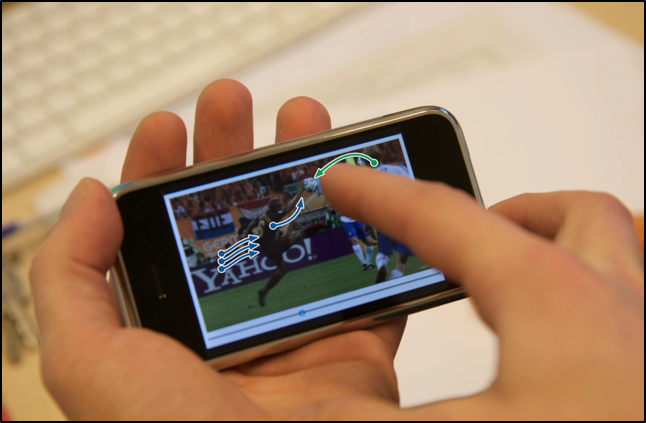
\includegraphics[scale=1.2]{./images/11.png}
\caption{PocketDRAGON mit Fußballszene \cite{karrer2009pocketdragon}}
\label{pocket_dragon}
\end{center}
\end{figure}Da die Leistung der mobilen Geräte nicht ausreicht, werden die besonders rechenintensiven Algorithmen extern auf einem angeschlossenen Server ausgeführt. Da das iPhone mittels Netzwerkkommunikation die Daten mit dem Server austauscht, kommt es zu Verzögerungen bei der Navigation. Diese konnte jedoch durch einen eigens für diesen Zweck entwickelten Algorithmus, welcher flexibel die einzelnen Frames zwischenspeichert und zur Vorschau lädt, minimiert werden. Des Weiteren werden die Videoframes in verschiedenen Auflösungen vorgeladen, sodass bei groben Bewegungen die Frames gezeigt werden, welche eine niedrige Auflösung haben und bei langsamen, detaillierteren Bewegungen, diese mit hoher Auflösung. Abbildung 3.7 zeigt die Bedienung des PocketDRAGON, mit einer Szene aus einem Fußballspiel. Auf dem Bild ist gut zu erkennen, wie der Nutzer mit dem Finger den Ball festhält und ihn genau an die Stelle seines Interesses bewegt. Die vorgestellte Version ist jedoch nicht in der Lage diese Navigationsmethode über eine längere Sequenz des Videos durchzuführen, sondern eignet sich nur, um Szenen mit kürzerer länge in detaillierter Weise zu betrachten. Eine klassische Navigationsleiste für das schnelle Bewegen wird zusätzlich unterhalb angezeigt. Das Ziel dieses Projektes war es nicht eine sogenannte Standalone Applikation zu schaffen, welche Marktreife hat, sondern um festzustellen, ob das Bedienkonzept auf Smartphones und Tablets sinnvoll ist. Eine Benutzerstudie wurde nicht durchgeführt, weshalb sich keine gültige Aussage darüber treffen lässt. \cite{karrer2009pocketdragon}

Der \emph{Keyframe Navigation Tree} von Hudelist, Schöffmann und Xu ist ein Prototyp für einen Videoplayer mit einer erweiterten Navigationsleiste. Diese besteht im Prinzip aus drei einzelnen Leisten, die sich oberhalb mit einander verbunden sind. Die oberste Navigationsleiste zeigt eine Reihe von sogenannten Keyframes, also Bilder aufgrund ihrer Position und Qualität besonders viele Informationen über den Inhalt des Videos liefern. Diese werden jedoch nicht vollständig dargestellt, sondern vertikale Ausschnitte, die alle direkt aneinander gelegt sind. Von links nach rechts ergibt sich somit eine Reihe dieser Keyframes, welche chronologisch beginnend vom Anfang des Videos extrahiert wurden. Die zweite Navigationsleiste darunter funktioniert nach den selben Prinzip. Hier sind die einzelnen Vorschaubilder etwas größer, was einen tieferen Einblick in den Inhalt zulässt. Das hat zufolge, dass diese Übersicht nur einen Ausschnitt des gesamten Videos zeigt.
\begin{figure}[h]
\begin{center}
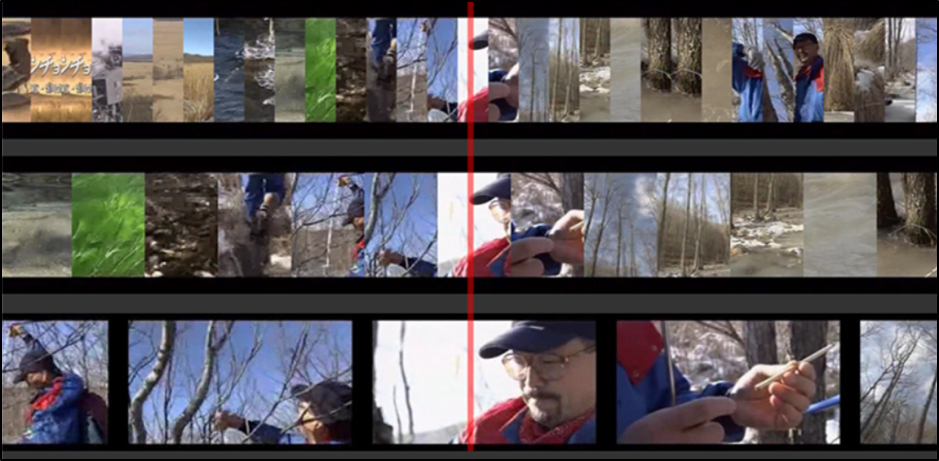
\includegraphics[scale=0.9]{./images/12.png}
\caption{Keyframe-basierter Navigationsbaum \cite{hudelist2015improving}}
\label{keyframe_tree}
\end{center}
\end{figure}
Die unterste Navigationsleiste zeigt dann die Vorschaubilder im vollen Umfang an und ist daher am genausten. Abbildung 3.8 zeigt eine Übersicht dieser Zeitleiste. Die rote durchgezogene Linie markiert die Stelle, an die das Video gerade abgespielt wird. Da die verschiedenen Leisten immer den selben Inhalt angeben, jedoch in unterschiedlicher Detailstufe, ist der rote Markierer für alle Leisten gültig. Mit dem Finger können alle drei Bereiche unabhängig voneinander bewegt werden, was das Video nach vorne, bzw. hinten navigieren lässt. Sobald der Finger vom Bildschirm gelöst wird, spielt das Video an dieser Stelle dann ab. Eine Benutzerstudie welche Im Rahmen dieses Projekts durchgeführt wurde, kam zu dem Schluss, dass die Teilnehmer die Navigation als viel einfacher und intuitiver wahrgenommen haben, die gestellten Suchaufgaben schneller lösen konnten und auch mehr Spaß machte. Insgesamt haben nur 3 von den 20 Kandidaten den Standardvideoplayer bevorzugt, gegen den die Vergleichsmessung durchgeführt wurde. \cite{hudelist2015improving}

Der \emph{Mobile ZoomSlider} von Hürst, Götz und Welte verfolgt den Ansatz eine Navigation ohne fixer Zeitleiste zu ermöglichen. Hierbei ist der Gedanke, dass der Nutzer überall auf den Bildschirm tippen kann und sich an dieser Stelle die Funktion einer Navigationsleiste aktiviert. Der große Vorteil dabei ist, dass kleine Knöpfe auf einem Schieberegler nicht mühsam angepeilt werden müssen. Die horizontale Bewegung bestimmt, ob im Video nach vorne oder hinten navigiert wird und die vertikale Position des Eingabestifts gibt an, wie schnell man sich im Video bewegt. Daher auch der Name ZoomSlider, da die vertikale Bewegung die Zeitleiste entweder vergrößert oder verkleinert. Als zusätzliche Funktion wurden sogenannte Speedborders implementiert. Das bedeutet, dass der Nutzer an die rechte oder linke Kante drücken kann, um einen Schnellvorlauf, bzw. Rücklauf zu aktivieren. Auch wurde wieder die vertikale Position des Stiftes mit einbezogen, sodass der Schnelllauf weiter oben langsamer ist, verglichen zum unteren Bereich. Damit der Nutzer immer weiß, welche Auswirkungen seine Aktionen haben, werden unterschiedliche visuelle Feedbacks gegeben.
\begin{figure}[h]
\begin{center}
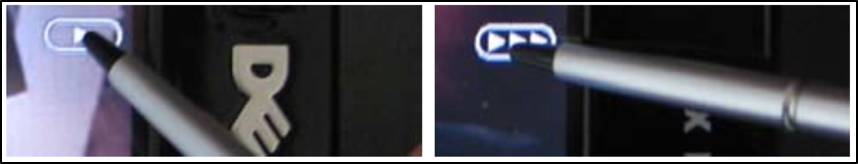
\includegraphics[scale=1]{./images/13.png}
\caption{Mobile ZoomSlider Schnelldurchlauf durch Speedborders \cite{hurst2007interactive}}
\label{mobile_zoomslider}
\end{center}
\end{figure}
In Abbildung 3.9 sind beispielsweise die Symbole zu sehen, welche beim Schnelldurchlauf eingeblendet werden. Hier ist zusätzlich noch anzumerken, dass die Symbole immer an der Stelle eingeblendet werden, an der der Stift den Bildschirm berührt. Im Zuge der Implementierung wurde im Anschluss der Mobile ZoomSlider mittels Benutzerstudie evaluiert. Zu Beginn haben die Teilnehmer eine kurze Einführung in die Handhabung des Videoplayers bekommen. Ziel der Studie war es herauszufinden, wie gut die Probanden die Navigationsmethode verstehen und ob sie damit Suchaufgaben lösen könnten. Des Weiteren wurden die subjektiven Eindrücke festgehalten. Die Ergebnisse waren, dass die Bedienbarkeit als natürlich und positiv empfunden wurde, sowie eine steile Lernkurve verzeichnet werden konnte. Die Suchaufgaben konnten ebenfalls gut gelöst werden. \cite{hurst2007interactive}

Das nächste Beispiel eines mobilen Videobrowsers ist dafür vorgesehen, dass man sich sowohl innerhalb eines Videos, als auch zwischen verschiedenen Videos navigieren kann. Der \emph{Wipe’n’Watch} Player von Huber et al. ist eine iPhone Applikation, die speziell für den Fall von eLearning Material entwickelt wurde. Das bedeutet, dass die verwendeten Videomaterialen in der Regel Aufzeichnungen von Universitätsvorlesungen sind. Diese zeigen nur die präsentierten Folien als visuelles Objekt und die Audiospur ist der Kommentar des Vortragenden. Anstatt aber eine Zeitleiste zu benutzen, springt man immer zum Keyframe. Dies geschieht mit einem horizontalen Wisch. Die Richtung der Bewegung gibt an, ob man sich nach vorne oder nach hinten bewegt. Da die Videos nur die Vorlesungsfolien anzeigen, sind die Keyframes also immer der Beginn einer neuen Folie. So springt man also beim navigieren immer von einer Folie zur nächste im Video und die Audiospur passt sich dementsprechend an. Somit ist es möglich das Video wie eine PDF Datei zu lesen und zu navigieren. Beim Wipe’n’Watch Player werden Videos mit Hyperlinks verwendet, die auch Hypervideos genannt werden. Das bedeutet, dass an verschiedenen Stellen im Video Links zu anderen Videos sind, die semantisch miteinander zusammenhängen.
\begin{figure}[h]
\begin{center}
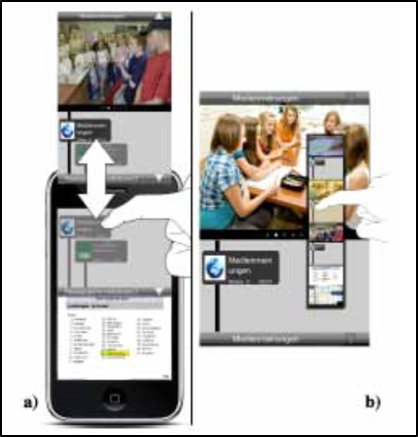
\includegraphics[scale=1.2]{./images/14.png}
\caption{Wipe'n'Watch Player mit inter-Video Navigation \cite{huber2010wipe}}
\label{wipenwatch}
\end{center}
\end{figure}
Sobald eine Folie angezeigt wird, welche also inhaltlich mit einem oder mehreren Videos zusammenhängt, wird ein kleines Symbol eingeblendet. In diesem Fall kann der Nutzer mit einem vertikalen Wisch nach oben eine Übersicht mit allen dieser Videos öffnen. Die Abbildung 3.10 zeigt, wie diese Interaktion auf einem Gerät aussieht. Auf dem Bild a) sind zwei referenzierte Videos in der Übersicht enthalten, zu erkennen da sie sich in der grauen Box befinden. Mit einem Klick auf eines der Videos wird dieses abgespielt. Mit einem Wisch nach unten wird die Übersicht wieder geschlossen. Ein langer Druck auf den Bildschirm öffnet den Verlauf der letzten Videos, was in Abbildung 3.10 b) zu sehen ist. Eine Benutzerstudie mit 44 Probanden hat gezeigt, dass komplexe Suchaufgaben mit den Wipe’n’Watch Player schneller gelöst werden konnte, im Vergleich zu einem nur leicht veränderten Standardvideoplayer. Zudem wurde ein hohes Verständnis für die Zusammenhänge der Videos geschaffen, sowie positives zur Benutzerfreundlichkeit beigetragen. \cite{huber2010wipe}

Ein Videobrowser, welcher auf einem ähnlichen Navigationsprinzip aufbaut, ist der \emph{SwiPlayer} von Schöffmann, Chromik und Böszörményi. Auch hier werden horizontale und vertikale Wischgesten benutzt, um sich innerhalb eines Videos, bzw. zwischen verschiedenen Videos zu bewegen. Der Videoplayer ist jedoch nicht für eine bestimmten Videotyp ausgelegt, sondern für jede Art gleichermaßen geeignet. Die Bedienkonzept geht dabei so vor, dass eine Navigationsleiste vollkommen ausgelassen wurde und nur die direkte Interaktion mit dem Video im Vordergrund steht. Ähnlich wie bei einem Fotoalben Applikation auf dem Smartphone oder Tablet kann man das angezeigte Bild nach rechts oder links wegwischen, um zum nächsten bzw. vorherigen Bild zu gelangen. Nur dass in diesem Fall keine Bilder betrachtet werden, sondern der Inhalt eines Videos. Wenn der Nutzer also den Bildschirm berührt, dann pausiert das Video, bis es wieder losgelassen wurde.
\begin{figure}[h]
\begin{center}
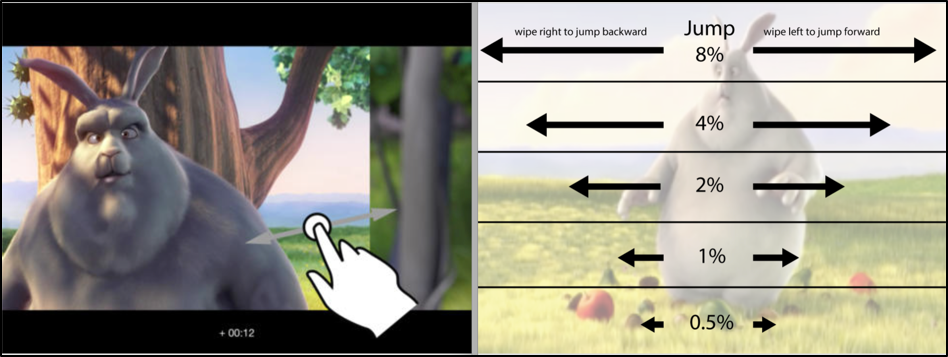
\includegraphics[scale=0.9]{./images/15.png}
\caption{SwiPlayer intra-Video Navigation und Granularität \cite{schoeffmann2014video2}}
\label{swiplayer}
\end{center}
\end{figure}
In Abbildung 3.11 (links) ist zu sehen, wie das Video von rechts nach links geschoben wird. Währenddessen bewegt sich von rechts die neue Position ins Bild, an der das Video dann weitergeht. Um eine Verfeinerung der Navigation zu ermöglichen, ist die Sprungweite immer prozentual von der Videolänge abhängig. Dieser Prozentwert variiert je nach vertikaler Position des Fingers. Wie in Abbildung 3.11 (rechts) zu sehen ist, gibt es insgesamt 5 verschiedene Werte, die angenommen werden können. Grobe Sprünge von 8\% können oben erreicht werden, bis zu feineren 0,5\% am unteren Bildschirmrand. Der Nutzer hat jederzeit die Möglichkeit die Aktion abzubrechen, indem er die Bewegung nicht vollständig ausführt, den Finger also anhebt und der Videoplayer sich somit wieder auf die ursprüngliche Position ausrichtet und die Wiedergabe fortsetzt. Falls das Video von Beginn an in pausiertem Modus war, dann würde das Video nicht sofort laufen, sondern muss manuell mit einem 2-Finger Tippen die Wiedergabe starten. Ein vertikaler Wisch von unten nach oben hat zur Folge, dass das nächste Video in der Sammlung gespielt wird. Die letzte Position des vorherigen Videos wird jedoch gespeichert, sodass der Nutzer dort fortfahren kann. Somit ist es möglich, ähnlich wie bei dem ThumbBrowser, den SwiPlayer ausschließlich mit den Daumen zu bedienen. Für eine Evaluierung wurde im Rahmen des Projektes eine Benutzerstudie durchgeführt. Dort wurde der Prototyp des Videoplayers mit dem Standardvideoplayer des iPads verglichen. Insgesamt 24 Probanden haben mehrere Known-Items-Search-Tasks gemacht, sowohl mit dem SwiPlayer, als auch mit dem Standardplayer. Die Ergebnisse waren, dass die Suchaufgaben mit dem wischgesten-basierten Player etwas schneller fertiggestellt werden konnten. Die subjektive Wahrnehmung der Nutzer war, dass die Navigationsmethode sehr schnell zu erlernen sei und 87\% der Teilnehmer diesen Videobrowser für das Erfüllen der Aufgaben bevorzugten. \cite{schoeffmann2014video2}

In diesem Kapitel wurden nun einige Ansätze vorgestellt, wie Videonavigation bzw. Videobrowsing auf Smartphones und Tablets umgesetzt werden kann. Die verschiedenen Prototypen verwendeten teilweise Methoden aus Video Retrieval, beispielsweise, um Keyframes aus dem Video zu identifizieren, oder um den Bewegungsverlauf von Objekten aufzuzeichnen. Jedoch war eine Kombination mit einer veränderten Darstellung des Inhaltes oder Navigationshilfen wie Gesten immer notwendig, um einen tatsächlichen Vorteil zu generieren. Die gewonnenen Erkenntnisse, insbesondere des SwiPlayers waren Anlass und Ideengeber für den Prototypen, der im Rahmen dieser Arbeit umgesetzt wurde.

\chapter{Wischgestenbasierender Videoplayer}

In den vorherigen Kapiteln wurden verschiedene Navigationsmethoden von Videoplayer vorgestellt. Diese waren sowohl aus dem Bereich der Desktop-Computer, sowie mobile Geräte wie Smartphones und Tablets. Letztere bieten mit ihren präzisen Touchscreens besondere Möglichkeiten. Im Rahmen dieser Arbeit wurde ein Prototyp eines Videoplayers entwickelt, welcher ausschließlich mit Wischgesten den Nutzer durch ein Video navigieren lässt. Im weiteren Verlauf der Arbeit wird dieser als Flickplayer bezeichnet. Der Name Flick kommt aus dem Englischen und bedeutet so viel wie etwas schnippen oder schnellen lassen. Insofern ist das passend, da dies die Bewegung beschreibt, die bei der Navigation angewendet werden muss. In diesem Kapitel wird der gesamte Entwicklungsprozess der Prototypen beschrieben. Beginnend von der Spezifikation, bis hin zu Details bezüglich der Implementierung.

\section{Spezifikation}

Bevor mit der Implementierung begonnen werden konnte, musste zuerst genau ausgearbeitet werden, wie das Navigationskonzept funktionieren und die Benutzeroberfläche gestaltet werden sollte. Die Einzelheiten zur Konzeptionsphase werden deshalb in diesem Kapitel aufgearbeitet.

\subsection{Anforderungsanalyse}

Wischgestenbasierte Videoplayer haben oft das Problem, dass in unterschiedlicher Weise von einer Szene in die nächste gesprungen wird. Dabei wird ein Teil des Inhalts oft übersprungen, da der Nutzer diesen gar nicht zu sehen bekommt. Als Grundlage wurde der SwiPlayer genommen, da hier im Rahmen einer Nutzerstudie herausgefunden wurde, dass das Bedienkonzept bei der Navigation unterstützte und sehr positiv von den Probanden bewertet wurde. Jedoch gab es genau hier die Limitierung, dass zwischen den einzelnen Szenen der Inhalt übersprungen werden konnte. Dieses Problem sollte mit dem Flickplayer gelöst werden. Des Weiteren sollte die Benutzeroberfläche sehr einfach gestaltet werden, sodass eine Ablenkung durch viele Bedienelemente verhindern werden kann. Daher eignen sich Wischgesten sehr gut, da somit auf Knöpfe verzichtet wird. Der Flickplayer sollte zudem in der Lage seine, eine Navigation sowohl nach vorne im Video, sowie rückwärts zuzulassen.

\subsection{Navigationskonzept}

Beim Navigationskonzept werden horizontale Wischgesten benutzt, um sich innerhalb eines Videos zu bewegen. Dabei werden jedoch keine sprunghaften Bewegungen auf der Zeitleiste gemacht, sondern die Wiedergabegeschwindigkeit des Videos dynamisch verändert. Standardmäßig werden Videos mit einer Geschwindigkeit von 100\% abgespielt. Da auf eine Navigationsleiste bewusst verzichtet werden sollte, kann der Nutzer die Wiedergabegeschwindigkeit auf bis zu 32-fach bringen, also 3200\%, um sich schnell im Video bewegen zu können. Der große Vorteil hierbei ist, dass man so von trotzdem beschleunigter Navigation dennoch einen Eindruck vom Inhalt des Videos bekommt. Das eigentliche Konzept hat starke Parallelen zur Navigation innerhalb von Listen auf Smartphones. Anstatt von Seiten, zwischen denen umgeblättert wird, kann der Inhalt festgehalten werden und schwungartig nach oben oder unten bewegt werden. Diese Navigationsart wird auch Scrolling genannt.
\begin{figure}[h]
\begin{center}
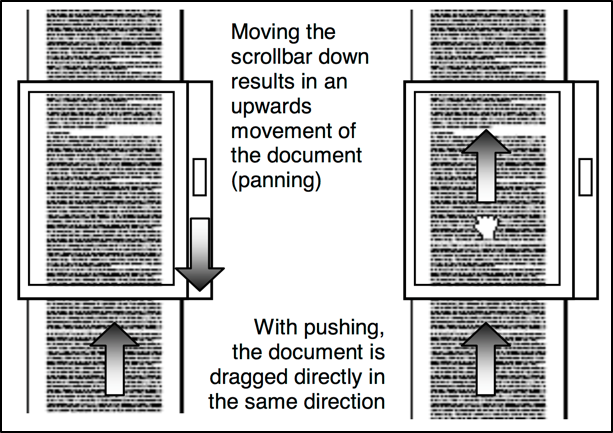
\includegraphics[scale=1.1]{./images/16.png}
\caption{Navigation innerhalb von Textdokumenten \cite{hurst2008interfaces}}
\label{scrolling_text}
\end{center}
\end{figure}
Die unten gezeigte Abbildung 4.1 veranschaulicht dieses Scrolling innerhalb eines Dokuments. Die einzelnen Seiten werden übergangslos aneinandergehängt, sodass der Nutzer mit einer Wischbewegung schnell über mehrere Seiten navigieren kann \cite{hurst2008interfaces}. Bei dem Prototyp des Flickplayers wird daher die Wiedergabegeschwindigkeit des Videos angepasst. Um den Übergang von der 1-fachen Geschwindigkeit, bis hin zum Maximum, also 32-fachen Geschwindigkeit nicht ruckartig zu machen, gib es mehreren Zwischenstufen als Übergänge. Diese sind 2-fach, 4-fach, 8-fach und 16-fach. Wie bei dem Scrolling eines Dokumentes hat ein stärkerer Wisch einen größeren Effekt, als ein leichter, bzw. langsamerer Wisch. Die Übergänge zwischen den Abspielgeschwindigkeiten sollten somit für den Nutzer als flüssig wahrgenommen werden. Die gleichen Intervalle wurden ebenso für das rückwärts abspielen übernommen, sodass ein einheitliches Konzept entsteht. Ein Wisch von links nach rechts hat somit zur Folge, dass sich das Video rückwärts abspielt, bis hin zu einer Geschwindigkeit von minus 32-fach.
\begin{figure}[h]
\begin{center}
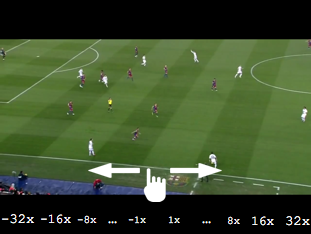
\includegraphics[scale=1.1]{./images/17.png}
\caption{Flickplayer Wischgesteninteraktion}
\label{finger_bild}
\end{center}
\end{figure}
In Abbildung 4.2 wird das Navigationskonzept nochmals grafisch dargestellt. Zu sehen ist ein Finger, welche die horizontale Bewegung andeutet, sowie die verschiedenen Stufen der Abspielgeschwindigkeit in beide Richtungen. Um von einer höheren Abspielgeschwindigkeit wieder in den Ausgangszustand zu gelangen hat der Nutzer verschiedene Möglichkeiten. Da bei einem Wisch von rechts nach links die Geschwindigkeit zunimmt, baut diese sich im Laufe der Zeit mit einer linearen Funktion wieder ab. Weitere Wischgesten in die selbe Richtung lassen den internen Wert weiter erhöhen. Dies ist so lange der Fall, bis das Maximum erreicht wird. Die Intervalle sind zwischen den Geschwindigkeit alle exakt gleichgroß, sodass im Fall des Maximums der Wert linear abnimmt und so alle Geschwindigkeitsstufen gleich lang aktiv sind. Eine lineare Funktion eignete sich hierbei an besten, da dies am transparentesten für die Nutzer war, was durch frühen nicht-dokumentierten Tests herauskam. Ein Wisch in die entgegengesetzte Richtung mindern diesen Wert schneller, sodass dieser irgendwann negativ wird und das Video rückwärts abgespielt wird. Der schnellste Weg, um wieder in die Ausgangssituation der 1-fachen Geschwindigkeit zu gelangen, ist ein einfacher Fingertipp auf den Bildschirm. Der intern verwendete Wert wird somit direkt auf null gesetzt. Das ist insbesondere hilfreich, wenn man eine bestimmte Szene versucht zu finden und mit hoher Geschwindigkeit durch das Video navigiert. Sobald man glaubt die Szene gefunden zu haben, stoppt man das schnelle Abspielen und kann so in 1-facher Geschwindigkeit die Szene genauer untersuchen. Wenn man am Ende des Videos angelangt ist, gelangt man automatisch wieder zum Anfang des Videos. Umgekehrt ist dies auch möglich, denn wenn der Nutzer ein Video startet und direkt zum Ende des Videos gelangen möchte, dann kann er das Video rückwärts abspielen. Sobald der Beginn erreicht wurde, springt man automatisch zum Ende.

\subsection{Grafische Benutzeroberfläche}

Die Benutzeroberfläche wurde so gestaltet, dass der Nutzer von den Elementen nicht abgelenkt wird und diese nur eine sekundäre Funktion als Unterstützung einnehmen. Grundsätzlich sollten auch nur die wichtigsten Elemente mit eingebracht werden. Der Nutzer muss zu jeder Zeit wissen können, an welcher Stelle er sich gerade befinden und in welchem Zustand der Navigation der Videoplayer ist, also wie schnell das Video gerade abgespielt wird. Das ist wichtig, da aufgrund des Inhaltes sich nicht immer erschließen lässt, wie schnell man das Video gerade abspielt. Insbesondere bei Videos mit wenig Bewegungen ist das der Fall. Die folgende Abbildung 4.3 zeigt den Flickplayer auf einem Apple iPad mit einem Fußballvideo und den verschiedenen Elementen.
\begin{figure}[h]
\begin{center}
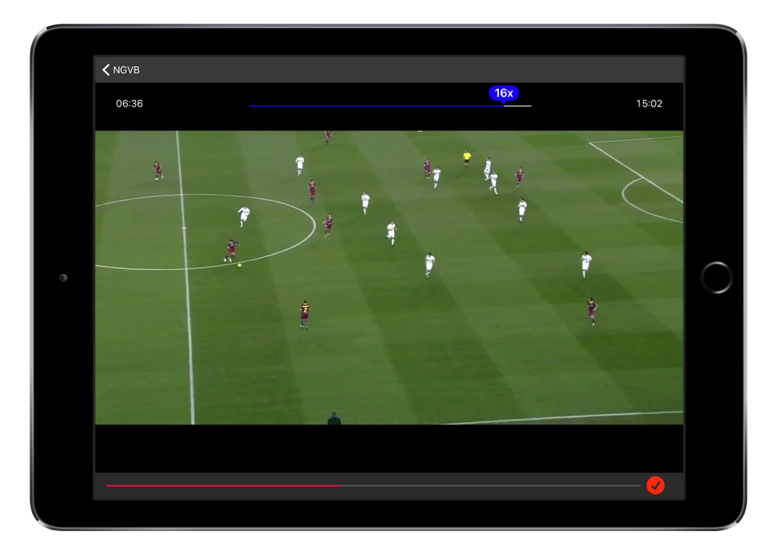
\includegraphics[scale=1.1]{./images/18.png}
\caption{Benutzeroberfläche des Flickplayers}
\label{flickplayer_gui}
\end{center}
\end{figure}
Am unteren Rand des Bildschirms ist eine Zeitleiste, welche mit einem roten Balken immer den aktuellen Fortschritt anzeigt. Diese Zeitleiste lässt sich jedoch nicht zur Navigation verwendet, wie dies bei den Standardvideoplayern üblich ist. Am oberen Rand werden in jeder Ecke jeweils noch ein Textlabel angezeigt. Das in der rechten Ecke gibt die gesamte Videolänge in Minuten und Sekunden wieder. Das Label in der linken oberen Ecke gibt immer die aktuelle Position wieder. Mittig am oberen Bildschirmrand ist ein Element, welches die aktuelle Wiedergabegeschwindigkeit anzeigt. Die Länge des Balkens gibt den gesamten Navigationsbereich ab. Ist der Balken bis zur Mitte hin gefüllt, bedeutet dies, dass der interne Wert bei 0 ist und die 1-fache Wiedergabe ist aktiv. Zusätzlich wird immer an der Stelle der aktuellen Füllmenge ein Indikator eingeblendet, welcher die Abspielgeschwindigkeit angibt. In der Abbildung liegt die momentane Geschwindigkeit bei 16-facher Rate. Mit diesen visuellen Elementen hat der Nutzer immer genauen Überblick über alle Parameter. Um das Nutzererlebnis zu verbessern wird bei einer schnelleren Abspielrate als der 1-fachen der Ton des Videos abgeschaltet, da dieser sehr unverständlich wird.

Wie die Anforderungen in der Implementierung umgesetzt wurden, wird im folgenden Kapitel detailliert dokumentiert.

\section{Details zur Implementierung und Probleme}

In diesem Kapitel wird die Implementierungsphase genauer beschrieben und die Probleme, die während der Umsetzung aufgetreten sind und wie diese gelöst wurden. Dabei wird auch die verwendete Hard- und Software, einzelne Klassen und Methoden bis hin zum Logging für die Benutzerstudie erläutert.

\subsection{Hardware und Software}

Die Zielplattform des Prototyps ist mit Apple iOS an bestimmte Hardware und Software gebunden. Da die Applikation einen erhöhten Ressourcenbedarf hat, war das Testgerät ein Apple iPad Air der ersten Generation. Zum Zeitpunkt der Implementierung war dies die aktuellste und leistungsstärkste iPad Version. Das Zielbetriebssystem war mit iOS 8 ebenfalls die aktuellste Softwareversion. Um Applikation für iOS zu entwickeln, ist man als Programmierer an Apple’s eigene Entwicklungsumgebung Xcode gebunden. Da die Umsetzung des Konzepts von Beginn an verschiedene Probleme zu bewältigen hatte, wurden verschiedene Ansätze konzipiert. Um diese unabhängig voneinander testen zu können, wurde das Versionierungssystem GIT verwendet. Dadurch konnte man mühelos zwischen den verschiedenen Versionen wechseln, ohne dass die unterschiedlichen Codefragmente Auswirkungen aufeinander haben. Des Weiteren wurde das Repository auf der Codehosting Plattform Github hochgeladen, sodass im Falle von Defekten auf dem Entwicklungsgerät kein Datenverlust auftreten kann und immer eine Kopie des Quellcodes vorhanden ist \cite{GithubLandingPage}. Eines der Probleme war die Kodierung der Videos, welches im Detail im Unterkapitel „Probleme“ weiter behandelt wird. Jedoch kann hier schon angemerkt werden, dass FFmpeg als Werkzeug verwendet wurde, um eines dieser Probleme zu lösen. FFmpeg ist ein plattform-übergreifendes, quell-offenes Projekt, welche eine Vielzahl von leistungsstarken Programmen und Softwarebibliotheken zusammenfasst, um Video und Audiodateien aufzunehmen, in verschiedene Formate umzuwandeln und zu manipulieren \cite{FFmpegLandingPage}. Das Tool an sich wir über die Kommandozeile bedient, wobei es mittlerweile auch Programme wie ffmpegx gibt, die eine Benutzeroberfläche haben und die wichtigsten Funktionen von FFmpeg so einfacher zu bedienen sind. \cite{granneman2010mac}

\subsection{Probleme}

Eines der Hauptprobleme während der Implementierung, war die geringe Leistungsfähigkeit des iPads. Die Video-Engine des AVFoundation Frameworks ist dahingehend limitiert, dass ein Video nur bis maximal 2-facher Geschwindigkeit abgespielt werden kann, ohne dass das Video ruckelt. Daher war der erste Ansatz, also auf Basis der Nutzerinteraktion die Abspielrate dynamisch anzupassen, so nicht mehr möglich. Die Videos mussten daher zuvor dahingehend bearbeitet werden, dass diese beschleunigt gespeichert wurden. Mit Hilfe von FFmpeg wurden die Videos mit 4-facher und 16-facher Geschwindigkeit kodiert, wodurch pro Video drei Videodateien benötigt wurden. Die Intervalle für die Abspielrate konnte so optimal abgedeckt werden, da beispielsweise das Video, welches in 16-facher Geschwindigkeit kodiert wurde, mit zweifacher Rate abgespielt werden konnte und so der Nutzer das zu betrachtende Video in 32-facher Geschwindigkeit wahrnimmt. Während der Wiedergabe musste dann zwischen den drei Dateien gewechselt werden, ohne dass dies dem Betrachter auffällt. Wie dies im Detail umgesetzt wurde, wird in den folgenden Kapiteln genauer erklärt. Ein weiteres Problem, welches es zu lösen galt, war die rückwärts-Wiedergabe. Ein Video besteht auf unterschiedlichen Arten von Einzelbilder. Im Einzelnen sind das die I-Frames, auch Inter-Frames genannt, welche unabhängig von anderen Einzelbildern die gesamte Information innehaben. Des Weiteren gibt es noch die P-Frames, welche nur Informationen über die Unterschiede zum vorherigen Bild speichern. Die sogenannten B-Frames speichern sowohl die Unterschiede zum vorherigen und zum nächsten Bild, wodurch eine besonders hohe Komprimierung erreicht werden kann. Nun gibt es das Problem, wenn man ein ganz bestimmtes Frame anzeigen möchte und dieses kein I-Frame ist, denn dann muss das letzte I-Frame als Startpunkt genommen werden und alle Frames in der Kette bis hin zum Ziel-Frame berechnet werden. In der folgenden Abbildung 4.10 ist diese Kette und die Abhängigkeiten zwischen den einzelnen Frames dargestellt. Alle Frames von einem I-Frame zum nächsten wird auch Group of Pictures, kurz GoP, genannt, was auf der Abbildung zu sehen ist \cite{wu2005guidelines}.
\begin{figure}[h]
\begin{center}
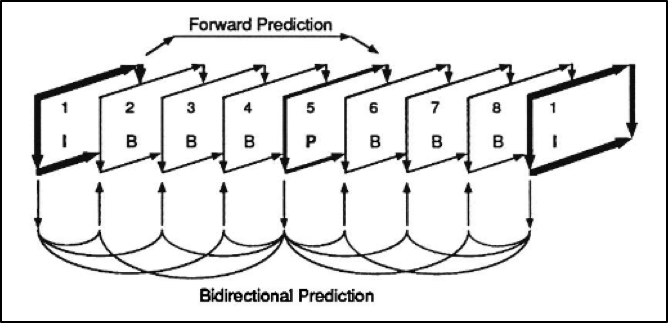
\includegraphics[scale=1.1]{./images/25.png}
\caption{Frame-Typen der Videokodierung \cite{wu2005guidelines}}
\label{gop_frames}
\end{center}
\end{figure}
Da die Berechnung der Zwischenframes einige Zeit dauert, kann das Video nicht ruckelfrei rückwärts abgespielt werden \cite{le1991mpeg}. Die Lösung hierfür war alle Videos zusätzlich so zu kodieren, dass sie nur aus I-Frames bestehen, sprich die GoP Größe wird auf 1 gesetzt. Dadurch war praktisch keine Komprimierung möglich, da jedes Frame ein Vollbild ist. Für das Evaluieren der Navigationsmethode war dies jedoch vollkommen ausreichend.

\subsection{Storyboard und Klassen}

In diesem Kapitel wird auf die Projektarchitektur eingegangen, also wie die Klassen und View Controller im Storyboard strukturiert sind, sowie kurze Erläuterungen zu wichtigen Methoden. Der Prototyp sollte sich nur die Anforderungen, welche in Kapitel 4.1 beschrieben wurde, fokussieren. Aus diesem Grund konnte die Projektgröße klein gehalten werden. Das gesamte Storyboard besteht, hier in Abbildung 4.11 zu sehen, aus zwei Einheiten. Zum einen ist das der Navigation Controller, welcher im Navigationstack die Übergänge und Navigation zwischen den verschiedenen View Controllern handhabt. An zweiter Position ist der Collection View zu sehen. Dieser gibt eine Übersicht über alle Videos, die von iTunes auf das iPad kopiert wurden, sodass diese zugänglich sind. Dieser Collection View enthält Zellen, eine für jedes verfügbare Video, jeweils mit einem Vorschaubild und dem Dateinamen. Das wichtigste Element im Storyboard ist der dritte View Controller der Abbildung. Dieser implementiert die Wiedergabe und Navigation des Flickplayers, also die Kernaufgabe der Applikation. Ein vierter View Controller ist ebenfalls auf dem Storyboard zu finden, dieser ist aber nur ein Eingabeformular für die Teilnehmerdaten der Benutzerstudie und hat keinen Einfluss auf die eigentlichen Navigation.
\begin{figure}[h]
\begin{center}
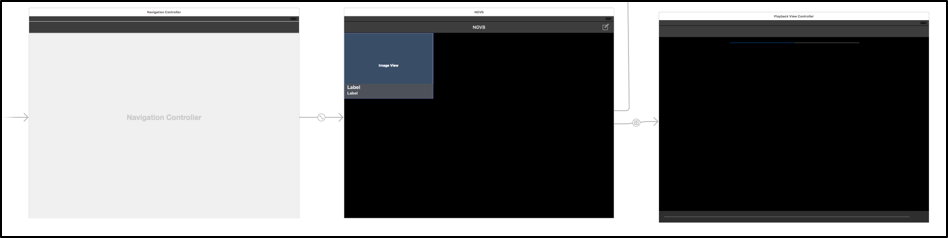
\includegraphics[scale=1]{./images/26.png}
\caption{Storyboard des Flickplayers}
\label{storyboard_flickplayer}
\end{center}
\end{figure}
Zu beiden View Controllern gibt es jeweils eine Klasse im Projekt, sowie eine Klasse für die Zelle im Collection View. Alle Klassennamen haben den Präfix VP, was eine Abkürzung für Videoplayer ist. Die wichtigste Methode in der Klasse VPCollectionViewController, ist dazu da, um alle Videos aus dem Dateisystem zu lesen.
\begin{lstlisting}
//get the iPod library
- (void) buildVideoLibrary {
	 itemList = [[NSMutableArray alloc] init];
	 MPMediaPropertyPredicate *predicate = [MPMediaPropertyPredicate predicateWithValue:[NSNumber numberWithInteger:MPMediaTypeHomeVideo] forProperty:MPMediaItemPropertyMediaType];
	 MPMediaQuery *query = [[MPMediaQuery alloc] init];
	 [query addFilterPredicate:predicate];
	 [itemList addObjectsFromArray:[query items]];
}
\end{lstlisting}
Das Attribut itemList wird hier zuerst initialisiert, bevor die Medienobjekte zugewiesen werden können. Um nicht alle Mediendateien vom System zu erhalten, muss ein Filter, auch predicate genannt, erstellt werden. Dazu wird ein Objekt der Klasse MPMediaPropertyPredicate initialisiert. Der Konstruktor verlangt dafür ein einen Filterwert, welcher aus der MPMediaType Enumeration stammt. Um Videos zu erhalten, die manuell über iTunes auf das Gerät kopiert wurden, muss der Wert MPMediaTypeHomeVideo übergeben werden. Anschließend wird dieser Filter einer MPMediaQuery Instanz übergeben. Dessen Attribut items hält nun alle Videos, die gesucht wurden \cite{MPMediaQueryClassReference}. Mit der Klasse AVAssetImageGenerator ist es nun möglich ein Vorschaubild der Videos zu erzeugen, die dann in den Zellen angezeigt werden können. Von der Collection View Zelle gibt es einen Segue, also eine Art Verknüpfung innerhalb des Storyboard zu einem anderen View Controller, welcher den eigentlich Video View Controller öffnet, um das jeweilige Video abzuspielen \cite{StoryboardSegue}. Beim Initialisieren des VPPlaybackViewController View Controllers werden noch nötige Attribute gesetzt. Diese sind die drei Video Dateien, in den verschiedenen Abspielgeschwindigkeiten 1-fach/4-fach/16-fach, die zum Abspielen eines Videos benötigt werden. In Kapitel 4.2.4 wurde erläutert, wie ein Videoplayer initialisiert und dem Hauptview des View Controllers zugewiesen werden muss. Beim Flickplayer übernimmt diese Aufgabe die Methode -(void)setupPlayers;, welche in der - (void)viewDidLoad; Methode aufgerufen wird. Jeder View Controller bietet einige Methode, die ausgeführt werden, wenn der View Controller beispielsweise geladen, in der Vordergrund kommt oder auch wieder geschlossen wird. Die viewDidLoad Methode wird immer dann ausgeführt, wenn der View Controller geladen wird, also noch bevor dieser angezeigt wird. In der Regel werden innerhalb diese Methode Vorbereitungen gemacht, wie Anpassen der Layout Elemente, oder wie am Beispiel des Flickplayers, das Laden der Videodateien und übergeben an die AVPlayer Instanzen \cite{UIViewControllerClass}. Neben kleineren Benutzerelementen werden hier auch die beiden Timer initialisiert, die für die Synchronisierung der drei Videoplayer zuständig sind, sowie automatische Anpassung der Abspielgeschwindigkeit. Wie dies im Detail umgesetzt wurde, wird im folgenden Kapitel genauer erläutert. Teil der Implementierung dieser Klasse, waren auch drei der Methoden aus der UIResponder Klasse. Diese sind:
\begin{itemize}
\item - (void)touchesBegan:(NSSet *)touches withEvent:(UIEvent *)event
\item - (void)touchesMoved:(NSSet *)touches withEvent:(UIEvent *)event
\item - (void)touchesEnded:(NSSet *)touches withEvent:(UIEvent *)event
\end{itemize}
Die touchesBegan Methode wird ausgeführt, sobald der Nutzer mit dem Finger den Bildschirm berührt. Das UIEvent event, welcher der Methode als Parameter übergeben wird, enthält alle Informationen, die benötigt werden. Das sind unter anderem die exakte Position auf dem Bildschirm, sowie der Zeitstempel, wann die Berührung gestartet wurde. Wie der Name der Methode schon vermuten lässt, wird diese Methode pro Interaktion genau einmal ausgeführt. Solange sich der oder die Finger auf dem Bildschirm bewegen, wird die Methode touchesMoved aufgerufen und zum Abschluss auch noch die Methode touchesEnded, wenn die Interaktion durch das Abheben des Fingers beendet wird. Welche Schritte innerhalb dieser Methoden ablaufen, wird ebenso im folgenden Kapitel genau ausgearbeitet. Der Videoplayer bietet wie in Kapitel 4.1.3 Elemente, die dem Nutzer dabei helfen eine Übersicht über die Position und Navigation zu erhalten. Diese Elemente werden ebenfalls in dieser Klasse geladen und aktualisiert. Die folgende Methode updateTimeLabel wird 12-mal pro Sekunde vom selben Timer aufgerufen, welcher die drei Videoplayer synchronisiert.

\begin{lstlisting}
-(void)updateTimeLabel {
    self.progressBar.progress = CMTimeGetSeconds(player1.currentTime)/CMTimeGetSeconds(playerItem1.duration);
    double seconds = CMTimeGetSeconds([player1 currentTime]);
    if (!isfinite(seconds)) {
        seconds = 0;
    }
    int secondsInt = round(seconds);
    int minutes = secondsInt/60;
    secondsInt -= minutes*60;
    int secondsIntDuration =
    round(CMTimeGetSeconds(player1.currentItem.duration));
    int minutesDuration = secondsIntDuration/60;
    secondsIntDuration -= minutesDuration*60;
    self.currentTimeLabel.text = [NSString stringWithFormat:@"%.2i:%.2i",minutes, secondsInt];
    self.totalLengthLabel.text = [NSString stringWithFormat:@"%.2i:%.2i",minutesDuration, secondsIntDuration];
}
\end{lstlisting}
Der UIProgressView progressBar wird zuerst auf den neusten Stand gebracht. Dabei wird der vom aktuell abgespielten Video die momentane Position genommen und durch die gesamte Videodauer geteilt. Daraus ergibt sich ein Prozentwert, welcher dann der progressBar als Wert zur Füllung übergeben wird. Des Weiteren werden in dieser Funktion die beiden Textlabel aktualisiert, die jeweils in die oberen Ecken positioniert sind. Dazu werden sowohl die gesamte Videodauer, sowie die momentane Position als Text umgewandelt, sodass diese Werte jeweils auf den Labels im mm:ss Format angezeigt werden kann.

Für die Statusanzeige der aktuellen Abspielgeschwindigkeit wurde, um die Komplexität einzugrenzen, auf ein Open Source Projekt zurückgegriffen. Der ASProgressPopUpView auf Github ist eine Subklasse der Standard-Progress Bar von iOS. Zusätzlich zum Auffüllen der Leiste, gibt es noch die Funktion ein Textlabel direkt an der Füllposition anzuheften, welches dynamisch den Text, sowie die Farbe anpassen kann. Die Farbanpassung, je nach Abspielgeschwindigkeit, sollte dem Nutzer als zusätzliche visuelle Hilfe die Navigation vereinfachen.
\begin{figure}[h]
\begin{center}
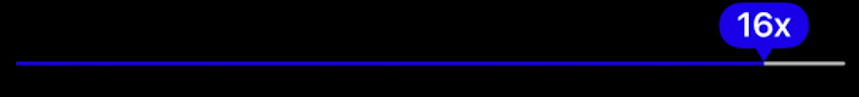
\includegraphics[scale=1]{./images/27.png}
\caption{Geschwindigkeitsindikator Flickplayer}
\label{flickplayer_indikator}
\end{center}
\end{figure}
Die Füllfarben für so gewählt, dass ein flüssiger Übergang von Rot nach Blau erfolgt, wie auch in der Abbildung 4.12 zu sehen ist.
\begin{lstlisting}
-(void)setupSpeedBar {
	self.progressViewMinus.popUpViewAnimatedColors = @[[UIColor redColor], [UIColor blueColor]];
	self.progressViewMinus.popUpViewCornerRadius = 10.0;
}
\end{lstlisting}
Zwischen der maximalen negativen und der maximalen positiven Geschwindigkeit gibt es insgesamt 12 Stufen. Der Timer, welcher die Geschwindigkeitsanpassung während der Navigation implementiert wird 20-mal pro Sekunde aufgerufen. Die ASProgressPopUpView Klasse verfügt über ein Protokoll, welches vom View Controller implementiert werden muss, um den Text zu aktualisieren. Sobald der Füllstatus sich verändert, wird die folgende Protokollmethode ausgeführt:
\begin{lstlisting}
- (NSString *)progressView:(ASProgressPopUpView *) progressView stringForProgress:(float)progress 
\end{lstlisting}
Als Übergabeparameter erhält der Methodenkörper der Prozentwert der Füllung. Mit einer einfachen Berechnung aller Intervalle mit x/12 wird dann überprüft in welchem Intervall dieser übergebene Werte sich befinden. Entsprechend wird dann der Text der Labels gesetzt. \cite{ASProgressPopUpViewRepository}
Im folgenden Kapitel wird im Detail aufgeführt wie die Navigation implementiert wurde.

\subsection{Umsetzung des Interaktionskonzepts}

Die Implementierung der Interaktionsmethode hatte einige Hürden, auf die schon in Kapitel 4.3.1 eingegangen wurde. Für die Umsetzung wurden verschiedene Methoden geschrieben, die beispielsweise die Videos synchronisieren, nach der Beschleunigung automatisch wieder die Geschwindigkeit auf 1-fache Abspielrate reduzieren, die drei verschiedene Views der einzelnen Videos in den Vordergrund bzw. Hintergrund zu schieben, sowie die Implementierungen der UIResponder-Methoden. Die Details dieser Methoden werden in diesem Kapitel verarbeitet.

Die Lösung für da Problem mit hohen Abspielraten wurde dahingehend gelöst, dass die Videos vorkodiert auf das Gerät übertragen wurden und dann übereinandergelegt wurden, sodass zwischen den einzelnen Videos hin und her geschalten werden konnte. Jedes UIView, welches jeweils ein Video hält, wurde so initialisiert, dass der Bildschirm vollständig ausgefüllt wird.
\begin{figure}[h]
\begin{center}
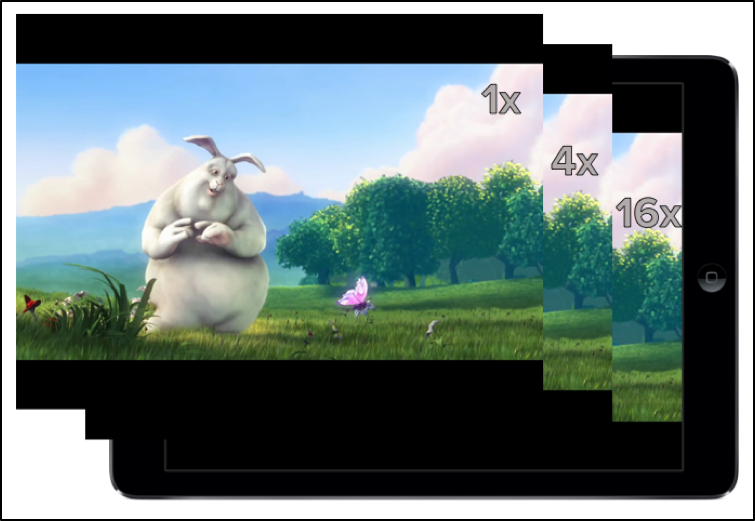
\includegraphics[scale=1.1]{./images/28.png}
\caption{Player View Stack}
\label{player_view_stack}
\end{center}
\end{figure}
In Abbildung 4.13 ist dargestellt wie die drei UIViews auf dem Bildschirm liegen, und welcher View, welches Video mit der jeweiligen Geschwindigkeit darstellt. Die UIResponder Events wird immer vom ersten UIView entgegengenommen, da diese Methoden für diesen View aber nicht implementiert wurden, werden diese durch die Stack Hierarchie weitergegeben, bis hin zum VPPlaybackViewController, welcher eine Unterklasse von UIViewController ist und somit auch ein UIResponder. Der VPPlaybackViewController hält ein Gleitkomma Attribut speed, welches der Zentrale Wert für die aktuelle Abspielgeschwindigkeit ist. In der touchesBegan Methode werden die Werte über die Position der Berührung auf der X-Achse gespeichert, sowie dessen Zeitpunkt. Die Y-Position kann hier bewusst vernachlässigt werden, da vertikale Wischgesten nicht verwendet werden. Wenn der Finger sich über den Bildschirm bewegt, dann wird bei jeder kleinen Zwischenbewegung die Methode touchesMoved aufgerufen.
\begin{lstlisting}
-(void)touchesMoved:(NSSet *)touches withEvent:(UIEvent *)event {
	 if (player1.rate != 0.0 || player2.rate != 0.0 || player3.rate != 0.0) {
	 	UITouch *touch = [[event allTouches] anyObject];
	 	CGPoint touchLocation = [touch locationInView:self.view];
	 	self.speed = self.speed - 3.3 * (touchLocation.x - self.position) / (event.timestamp - self.time);
	 	if (self.speed < -180000.0) {
		 	self.speed = -180000.0;
	 	} else if (self.speed > 180000.0) {
	 		self.speed = 180000.0;
	 	}
	 	self.time = event.timestamp;
	 	self.position = touchLocation.x;
    }
}
\end{lstlisting}
Der Videoplayer bietet auch eine Funktion, um die Videos zu pausieren. Aus diesem Grund wird zuerst überprüft, ob eines der Videos abgespielt wird. Falls nicht, dann wir diese Methode keine Auswirkungen haben. Ansonsten wird auch hier die X-Achsen Position gespeichert, um bei einem Vergleich zum vorherigen Wert aus der touchesBegan Methode festzustellen, in welche Richtung horizontal gewischt wurde. Die Bewegungsdistanz wird in Relation zum zeitlichen Abstand der Ereignisse gesetzt und das Ergebnis mit 3,3 multipliziert. Das Ergebnis aus dieser Gleichung wird zum aktuellen speed Wert addiert. Je nach Bewegungsrichtung kann das Ergebnis sowohl positiv, als auch negativ ausfallen. Der letzte Wert der X-Achsen Position, sowie der Zeitstempel werden immer gespeichert, um als Referenz verwendet zu werden, wenn die Bewegung weiter ausgeführt wird und so die touchesMoved Methode wieder aufgerufen wird. Um eine obere und untere Grenze zu schaffen, kann der speed nur Werte annehmen, die zwischen -180.000 und 180.000 liegen. Der Multiplikator wurde nicht zufällig gewählt, sondern wurde in kurzen Zwischentest mit Probanden so lange angenähert, bis eine positive Rückmeldung von den Nutzern kam, dass diese Konfiguration am angenehmsten zu verwenden ist. Denn umso höher dieser Multiplikator ist, desto einfacher ist es möglich auf die maximale Abspielrate von 3200\% zu gelangen.

Damit der speed Wert auch ohne Benutzereingabe von alleine wieder in den Ausgangszustand kommt, gibt es eine Easing-Funktion, die diesen linear reduziert. Hier wurden vom einem Extrem zum Nullpunkt insgesamt 12 gleichgroße Intervalle definiert. Innerhalb einer Sekunde wird der Wert 20-mal um 750 reduziert, sodass nach maximal 12 Sekunden wieder der Normal-Zustand angenommen und das Video in einfacher Rate abgespielt wird. Bei jedem Aufruf der Easing-Funktion, wird nach Ausführung berechnet, welcher Videoplayer aktiv sein sollte und mit welcher Geschwindigkeit dieser seinen Inhalt wiedergeben soll, dabei wird das Attribut activePlayer gesetzt, welches einen Ganzzahlwert zwischen 1 und 6 annehmen kann. Dies entspricht den drei Videos, die mit 100\% und 200\% ihrer Abspielrate jeweils 2 Zustände annehmen können. Auf das Klassenattribut activePlayer wurde ein Key-Value Observer gesetzt, welche schon in Kapitel 4.2.3 genauer erläutert wurden. Sobald also sich der Wert des Attributs ändert, wird folgende Methode ausgeführt:
\begin{lstlisting}
-(void)observeValueForKeyPath:(NSString *)keyPath ofObject:(id)object change:(NSDictionary*)change context:(void*)context;
\end{lstlisting}
Der keyPath, welcher als Parameter mitgegeben wird, entspricht dann dem Attributnamen, auf welchem der Observer gesetzt wurde. In dieser Methode werden alle Informationen verarbeitet, um das Video abzuspielen, welches im Vordergrund sein sollte, sowie die dessen Abspielrate festzulegen. Zuerst wird in einer if-Anweisung geprüft, welcher Player der aktuelle Player sein muss. Beispielsweise kann das momentane aktive Intervall, also der activePlayer, gleich zwei sein. Das Bedeutet, dass das Video, welches in 1-facher Geschwindigkeit kodiert ist, in der Vordergrund kommt und die beiden anderen Videos pausiert werden. Des Weiteren gibt dieses Intervall an, dass die Rate auf 200\% gesetzt werden muss. Als Ergebnis ist das Video, welches in doppelter Geschwindigkeit dem Nutzer wiedergegeben wird. Falls der activePlayer die 4 ist, dann wird das 4-fach Video mit zweifacher Geschwindigkeit und somit 8-fach dem Nutzer präsentiert.
\begin{figure}[h]
\begin{center}
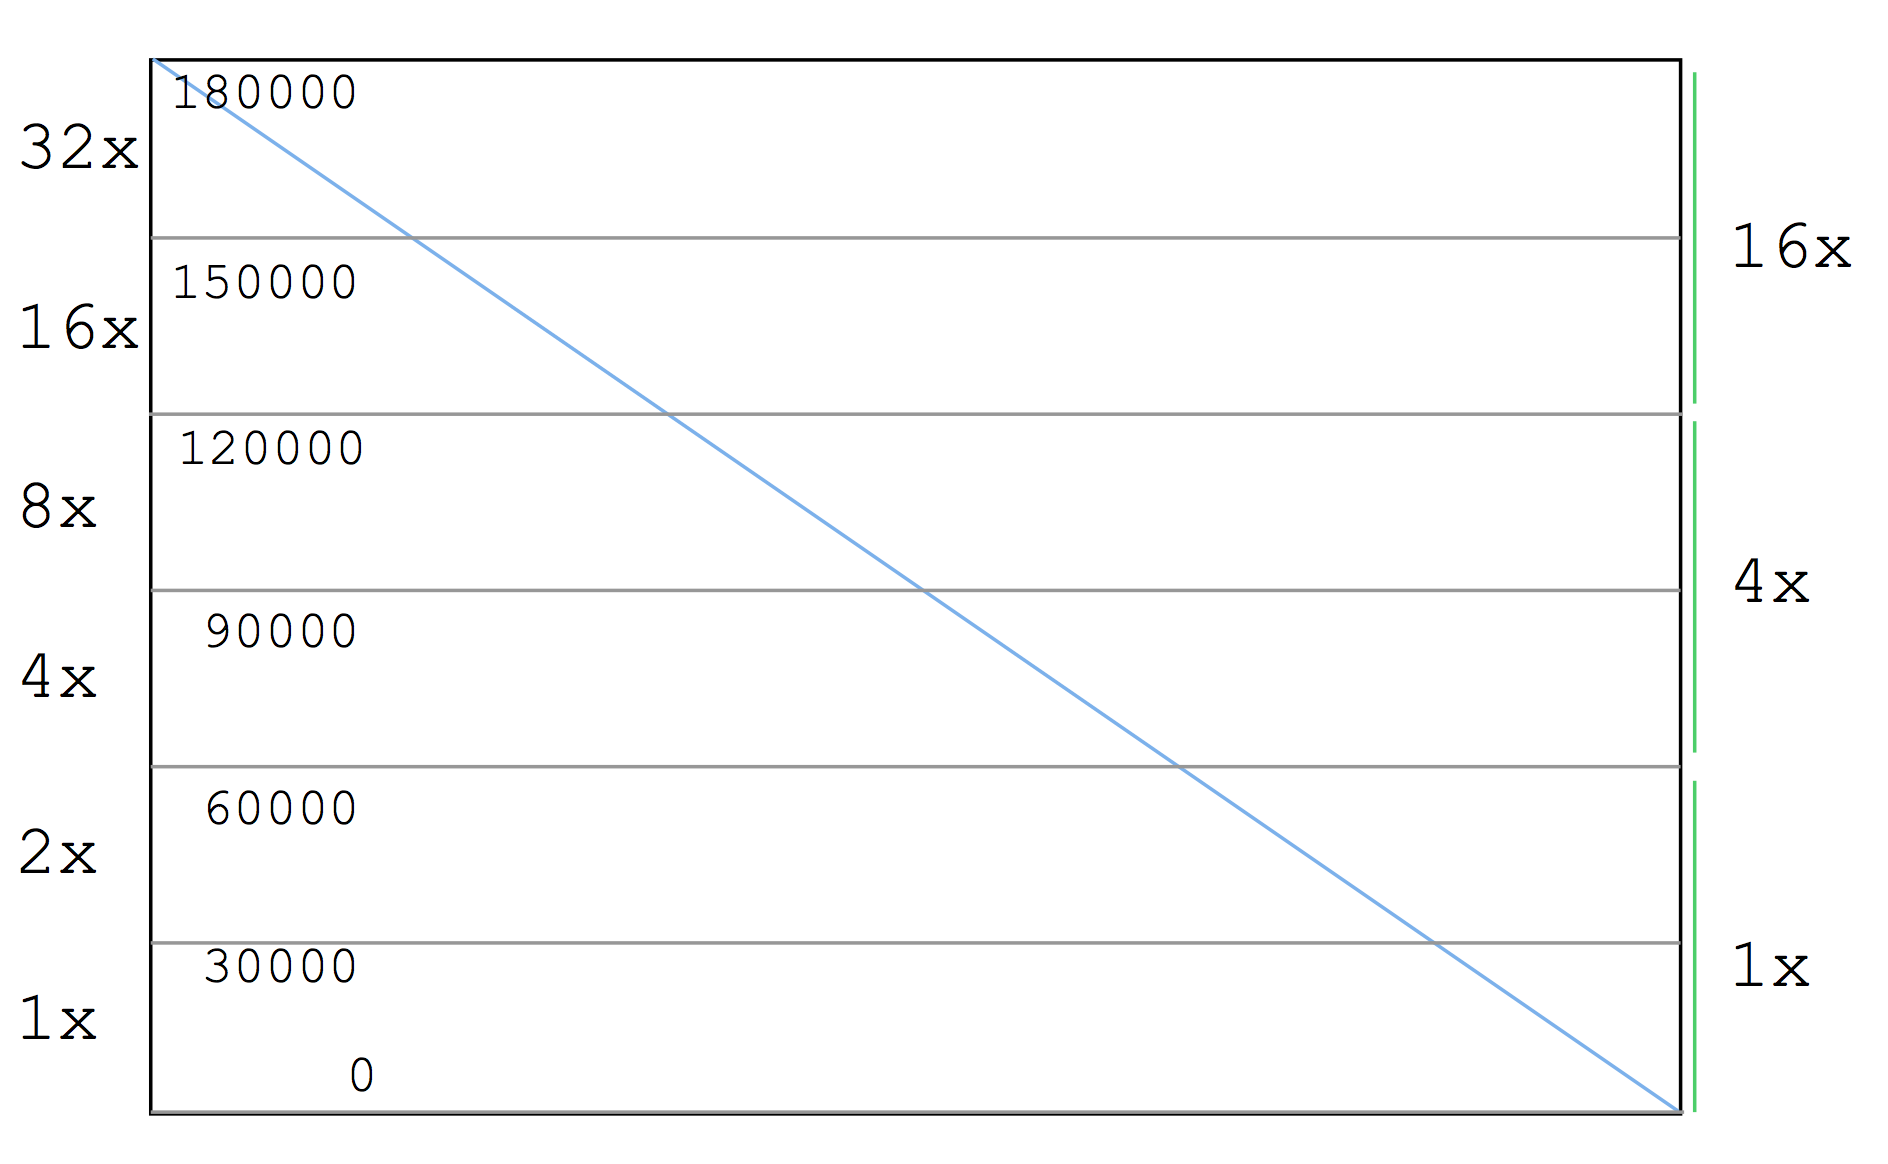
\includegraphics[scale=0.4]{./images/29.png}
\caption{Flickplayer Geschwindigkeits-Intervalle}
\label{flickplayer_interval}
\end{center}
\end{figure}
Die exakten Intervalle mit den verschiedenen Abspielgeschwindigkeiten, sind in Abbildung 4.14 grafisch dargestellt. Auf der linken Seite sind alle möglichen positiven Abspielrate aufgelistet. Ebenfalls zu sehen sind alle Intervalle von 0 bis 180.000, welche Werte vom Attribut speed sind. Auf der linken Seite die die drei Videos markiert und mit welcher Abspielrate diese Standardmäßig kodiert sind. Die Diagonale ist die Easing-Funktion, welche die Geschwindigkeit reduziert, falls der Nutzer keine Eingabe macht. Die gesamte Dauer der Linie vom Beginn, bis zum Nullpunkt entspricht 12 Sekunden. Somit wird jedes Intervall exakt zwei Sekunden wiedergegeben. Da das Video auch rückwärts abgespielt werden kann, ist das implementierte Prinzip vollständig in den negativen Bereich ausgebreitet, sodass die Grafik bis auf -180.000 ausgeweitet werden kann.

Das Foundation Framework bietet mit NSTimer eine Klasse, die über Instanz Methoden verfügt, um bestimmte Aktionen in einem zeitlichen Abstand einmal oder auch regelmäßig auszuführen \cite{NSTimerClass}. Beim Flickplayer wurde dies unter anderem eingesetzt, um die drei Videos miteinander synchron zu halten. Der NSTimer wurde dabei so initialisiert, dass der die Funktion adaptTimeStamps 12-mal in der Sekunde ausführt.
\begin{lstlisting}
defaultSpeedActivedTimer = [NSTimer scheduledTimerWithTimeInterval:1.5 target:self selector:@selector(defaultSpeedActived) userInfo:nil repeats:NO];
\end{lstlisting}
Da der Flickplayer immer nur das Video abspielt, welches gerade im Vordergrund erscheint, sind die anderen beiden pausiert. Um nun festzustellen, welche Videos in ihrer Position aktualisiert werden müssen, ist es notwendig herauszufinden, welches Video gerade abgespielt wird.
\begin{lstlisting}
- (void)adaptTimeStamps {
	CMTime videoPosition;
	Float64 videoPositionInSeconds;
	CMTimeScale scale = player1.currentItem.asset.duration.timescale;
	
	if (player1.rate != 0.0) {
		videoPosition = player1.currentTime; 
		videoPositionInSeconds = (Float64) videoPosition.value / videoPosition.timescale;
		CMTime time1 = CMTimeMakeWithSeconds(videoPositionInSeconds / 4.0, scale);
		CMTime time2 = CMTimeMakeWithSeconds(videoPositionInSeconds / 16.0, scale);
		[player2 seekToTime: time1 toleranceBefore: kCMTimeZero toleranceAfter: kCMTimeZero];
		[player3 seekToTime: time2 toleranceBefore: kCMTimeZero toleranceAfter: kCMTimeZero];        
	} else if (player2.rate != 0.0) {
		videoPosition = player2.currentTime; 
		videoPositionInSeconds = (Float64) videoPosition.value / videoPosition.timescale;
		CMTime time1 = CMTimeMakeWithSeconds(videoPositionInSeconds * 4.0, scale);
		CMTime time2 = CMTimeMakeWithSeconds(videoPositionInSeconds / 4.0, scale);
		[player1 seekToTime: time1 toleranceBefore: kCMTimeZero toleranceAfter: kCMTimeZero];
		[player3 seekToTime: time2 toleranceBefore: kCMTimeZero toleranceAfter: kCMTimeZero];        
	} else if (player3.rate != 0.0) {
		videoPosition = player3.currentTime;  
		videoPositionInSeconds = (Float64) videoPosition.value / videoPosition.timescale;
		CMTime time1 = CMTimeMakeWithSeconds(videoPositionInSeconds * 16.0, scale);
		CMTime time2 = CMTimeMakeWithSeconds(videoPositionInSeconds * 4.0, scale);
		[player1 seekToTime: time1 toleranceBefore: kCMTimeZero toleranceAfter: kCMTimeZero];
		[player2 seekToTime: time2 toleranceBefore: kCMTimeZero toleranceAfter: kCMTimeZero];
	}
	[self updateTimeLabel];
}
\end{lstlisting}
Mit einer if-Anweisung wird überprüft, welches Video nicht pausiert ist, also die Rate des AVPlayers nicht 0 ist. Die aktuelle Zeit des aktiven Videos wird erhalten und deren Basis und mit dem Umrechnungsfaktor die neue Position für die anderen beiden Videos errechnet. Beispielsweise wenn das erste Video gerade abgespielt wird, also das Video mit 1-facher Geschwindigkeit und an Stelle 16:00 ist, dann muss die aktuelle Zeit durch 4, bzw. 16 geteilt werden, um jeweils für die Videos mit 4- und 16-facher Geschwindigkeit den selben Inhalt wiederzugeben. Die Synchronisierung ist hauptsächlich dafür wichtig, dass beim Umschalten von einem zum anderen View ein flüssiger Übergang entsteht und der Nutzer dies nicht sehen kann.

Für die Benutzerstudie war es notwendig einen Logging-Mechanismus zu implementieren, sodass alle Nutzereingaben aufgezeichnet werden konnten. Somit konnte sichergestellt werden, dass zusätzlich zum Fragebogen, welche die subjektiven Eindrücke aufzeichnen sollte, zusätzlich noch quantitative Aussagen über die Leistungsfähigkeit des Flickplayers getroffen werden konnten.

\subsection{Logging}

Um die Daten später einfacher analysieren zu können, hat man sich dazu entschieden, die Daten in eine CSV Datei zu schreiben. CSV steht für Comma-seperated values und bedeutet, dass alle Werte mit einem Komma oder einem Semikolon getrennt werden. Des Weiteren werden die verschiedenen Datensätze mit jeweils mit einer neuen Zeile von einander getrennt. Der Vorteil dabei ist, dass die Daten in den üblichen Tabellenkalkulationsprogrammen geöffnet werden können \cite{louis2007java}. Um die Daten besser durchsuchen zu können, wurden die Log-Dateien in eine MySQL-Datenbank importiert, sodass mit SQL-Abfragen schneller gesucht werden konnte. Generell sollten so viele Information wie möglich während der Benutzerstudie gesammelt werden.

Bevor die der Nutzer mit den Aufgaben beginnen konnte, mussten einige Informationen zu dem jeweiligen Testlauf in ein Formular eingegeben werden, sodass die Daten jedem Nutzer, sowie der jeweiligen Aufgabe zugewiesen werden konnte. In Abbildung 4.15 ist eine Bildschirmaufnahme des Eingabeformulars zu sehen. Jeder Testkandidat das eine eindeutige ID erhalten, damit die ausgefüllten Fragebögen ebenfalls zugeordnet werden konnten. Des Weiteren wurde ein Schalter für die Auswahl der Aufgabenart angebracht. Dieser war notwendig, da sich die Benutzeroberfläche abhängig von der Aufgabe leicht unterschieden hatte. Um die Daten nicht alle in eine Datei zu speichern, konnte auf dem Eingabeformular ebenfalls ausgewählt werden, in welche der beiden Dateien die Testinformation gespeichert werden. Eine dritte Datei wurde ebenfalls angelegt, da jeder Nutzer vor dem Beginn der eigentlichen Aufgaben die Videoplayer schon benutzen konnten, um sich mit den verschiedenen Navigationsmethoden vertraut zu machen. Die Informationen aus dem Eingabeformular konnten nun gespeichert werden und das Video, somit auch das Logging, gestartet werden.
\begin{figure}[h]
\begin{center}
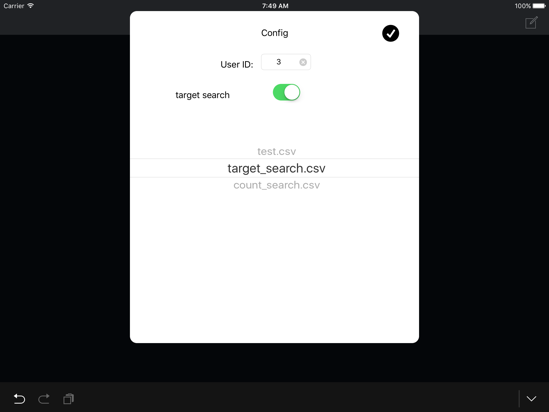
\includegraphics[scale=1.2]{./images/30.png}
\caption{Formular für Nutzertestinformationen}
\label{formular_logging}
\end{center}
\end{figure}
Das Video wird immer sofort gestartet, sobald es ausgewählt wurde. Der erste Logeintrag wird genau zu diesem Zeitpunkt erzeugt. Jeder Datensatz hat eine Vielzahl von Spalten, die hier im Einzelnen erläutert werden.
\begin{itemize}
\item ID – Jeder Datensatz hat eine eindeutige ID.
\item userID – Das ist die eindeutige Benutzer ID.
\item filename – Der Dateinamen, um danach die Daten der Aufgabe zuordnen zu können.
\item timestamp – Der genaue Zeitpunkt, an dem der Datensatz erzeugt wurde.
\item currenttime – Die aktuelle Position innerhalb des Videos.
\item playbackspeed – Die aktuelle Wiedergabegeschwindigkeit.
\item isplaying – Ist das aktuelle Video pausiert oder abgespielt wird.
\item pressed\textunderscore button – Ein Boolean, ob dieser Datensatz durch das Benutzen der Zähler ausgelöst wurde.
\item stepper\textunderscore 1, stepper\textunderscore 2, stepper\textunderscore 3, stepper\textunderscore 4 – Die Suchaufgaben für das Zählen von bestimmten Ereignissen boten einen Zähler für jedes Ereignis, welche auch in Abbildung 5.1 zu sehen sind. Diese Werte geben den aktuellen Zählstand wieder.
\item touch\textunderscore x - Die Fingerposition auf der horizontalen Ebene.
\item touch\textunderscore y – Die Fingerposition auf der vertikalen Ebene.
\item acceleration\textunderscore speed – Das ist der interne speed Wert.
\item finger\textunderscore touches\textunderscore screen – Ein Boolean, ob der Nutzer den Bildschirm gerade berührt.
\item start\textunderscore end – Der Datensatz ist ein Start-Datensatz, oder der Datensatz beim Beenden.
\end{itemize}
Die Aufgaben mit dem Standardplayer hatte noch eine Besonderheit, denn hier wurde die Granularität beim Benutzen der Navigationsleiste mitgespeichert. Die Datensätze wurden an verschiedenen Zeitpunkten erstellt. Der erste Eintrag wird erstellt, sobald das Video gestartet wird. Des Weiteren werden jeweils Logeinträge in den Methoden touchesBegan, touchesMoved und touchesEnded gespeichert. Bei den Aufgaben die Zähler benötigen, wird jeweils noch ein Eintrag geloggt, sobald einer der vier Zähler betätigt wurde. Beim Beenden der Aufgabe wird noch ein letzter Logeintrag gespeichert, um diesen zu kennzeichnen. Die Aufgaben, die mit dem Standardplayer durchgeführt wurden, erstellen Logeinträge, wenn der Nutzer die Navigationsleiste bediente, da hier die UIResponder Methoden nicht verwendet werden.

Der Aufbau der Studie, sowie deren Ausführung und Analyse der gewonnenen Daten werden im folgenden Kapitel genauer erörtert.

\chapter{Benutzerstudie und Evaluierung}

Um die Performanz des vorgeschlagenen Flickplayers zu messen, wurde im Rahmen der Arbeit eine Benutzerstudie durchgeführt. Dabei wurden den Probanden verschiedene Suchaufgaben gestellt, die sie sowohl mit dem Prototyp, als auch mit dem Standardplayer erledigen mussten. Durch den direkten Vergleich sollte sichergestellt werden, dass die Unterschiede zueinander Rückschlüsse auf die Effektivität und die Nutzerakzeptanz zulassen. Um so viele Daten wie möglich zu sammeln, wurde bei der Implementierung der Applikationen eine Logging-Funktion umgesetzt, welche alle Interaktionen der Benutzer mit den Videoplayern aufzeichnet. Zur Ergänzung wurde mithilfe eines zweiteiligen Fragebogens das subjektive Empfinden der Probanden festgehalten. Die Details des Versuchsaufbaus, die Durchführung und Analyse der gesammelten Daten werden in diesem Kapitel behandelt. Im Anschluss werden die gewonnenen Ergebnisse interpretiert und präsentiert.

\section{Aufbau der Studie}

Für die Durchführung der Studie wurden insgesamt 16 Probanden befragt. Jeder Benutzer musste sowohl Aufgaben mit dem Standardvideoplayer erledigen, als auch mit dem Prototyp des Videoplayers mit der Wischgestennavigation. Auf beiden Applikationen waren die selben 9 Videos verfügbar, wobei eines davon ein etwa 15 Minuten langes Testvideo war, mit dem die Nutzer sich mit den jeweiligen Navigationsmethoden vertraut machen konnten, bevor die eigentlichen Aufgaben durchgeführt wurden. Die Daten, die während des Testvideos aufgezeichnet wurden, sind aus der Analyse herausgelassen worden. Die Aufgaben lassen sich in zwei Kategorien einteilen. Zum einen Aufgaben aus dem Bereich “known-item-search”, also bei dem der Nutzer vor Beginn eine bestimmte Sequenz mit einer Länge von 20 Sekunden gezeigt bekommt und anschließend diese Szene in einem etwa 45 Minuten langem Video so schnell wie möglich finden muss, jedoch nicht weiß an welcher Stelle sich diese Szene befinden. Und zum anderen Suchaufgaben, bei denen in einem 15-minütigen Video vier verschiedene Ereignisse gezählt werden müssen, die beliebig oft vorkommen können. Der Grund für diese Auswahl der Aufgaben war, dass somit zum einen die Schnelligkeit untersucht werden kann, wie lange ein Nutzer braucht, um ihm bekannten Szenen ausfindig zu machen und zum anderen wie viel von den Inhalten der Videos aufgenommen wird, wenn der Nutzer mit teilweise stark erhöhter Abspielgeschwindigkeit durch die Videos navigiert.
\begin{figure}[h]
\begin{center}
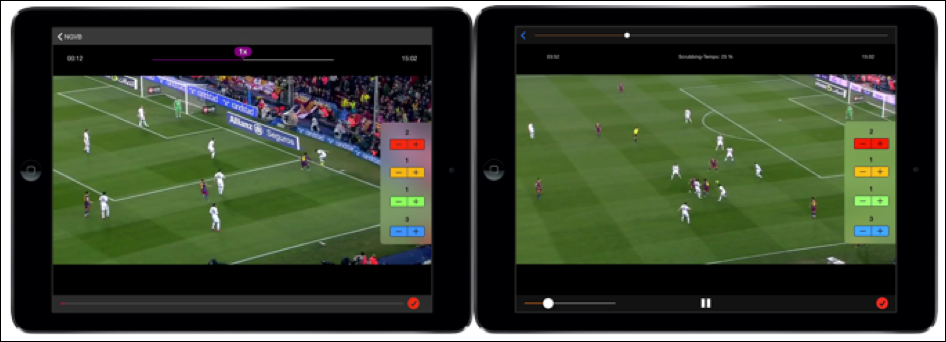
\includegraphics[scale=0.9]{./images/31.png}
\caption{Prototypen mit Adaptionen für Studie}
\label{prototyp_flickplayer_studie}
\end{center}
\end{figure}
Für die Suchaufgaben, bei denen die Nutzer vorgegebene Ereignisse finden und zählen müssen, wurden beide Videoplayer Applikationen um ein Widget ergänzt, mit denen das Zählen vorgenommen werden musste. Das betätigen der Zähl-Knöpfe wurden ebenfalls durch das Logging-System mitgeschrieben, sodass diese Daten einfacher und genauer ausgewertet werden konnten. Wenn der Nutzer die Aufgabe beenden möchte, dann ist dafür in der unteren rechten Ecke ein roter Knopf. Die Anzahl der Testpersonen wurde bewusst so gewählt, dass alle Permutationen der Aufgaben abgedeckt werden. In der folgenden Abbildung ist der exakte Versuchsaufbau detailliert dargestellt.
\begin{figure}[h]
\begin{center}
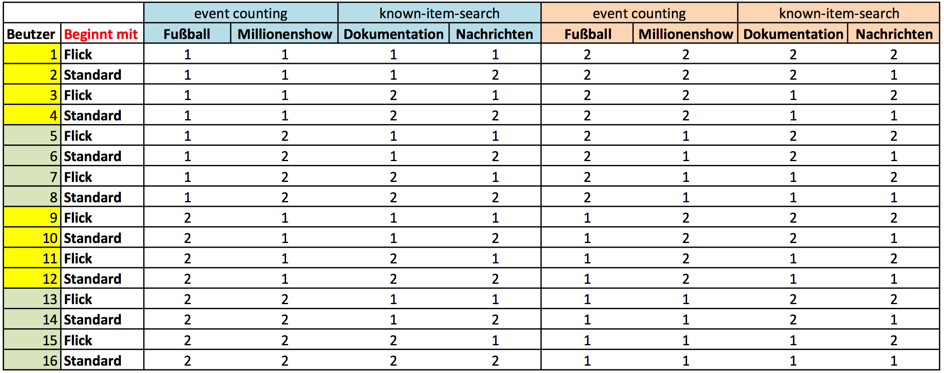
\includegraphics[scale=0.9]{./images/32.png}
\caption{Aufbau der Benutzerstudie}
\label{aufbau_studie}
\end{center}
\end{figure}
Insgesamt wurden acht verschiedene Videos in der Studie verwendet. Diese wurden in vier verschiedene Arten unterteilt, die da wären Fußball, Quizshow, Dokumentation und Nachrichten. Von jeder Art gab es jeweils zwei verschiedene Videos. Welches Video für welchen Videoplayer und welchen Testkandidaten verwendet wurde, kann in der Abbildung bei der Unterscheidung von 1 und 2 gesehen werden. Von Benutzer zu Benutzer wurde immer abgewechselt, mit welchem Videoplayer die Aufgaben zuerst bearbeitet werden mussten. Dies führte dazu, dass der erste Nutzer mit dem sogenannten Flick Player startete und der zweite Nutzer mit dem Standardplayer. Des Weiteren wurde ebenso schon zuvor definiert, mit welcher Art von Aufgaben begonnen werden musste. In der ersten Spalte kann dies zwischen den Farben Gelb und Grün erkannt werden. Gelb stand in dieser Studie für die known-item-search Aufgaben und Grün für die Aufgaben, bei denen die Probanden bestimmte Ereignisse zählen mussten. Damit die Testkandidaten ihr angeeignetes Wissen über die Videos nicht bei anderen Aufgaben anwenden können, wurde bei der Verteilung darauf geachtet, dass kein Kandidat ein Video mehrfach bearbeitet. Die Permutationen ergaben somit eine Anzahl von 16 Konfigurationen, die getestet werden mussten, um eine aussagekräftige Studie zu gewährleisten.

\section{Durchführung}

Für die Durchführung wurde ein schwarzes Apple iPad Air 1 mit einem 9,7 Zoll großen Bildschirm verwendet. Dabei wurden bei beiden Applikationen die Videos im Querbildformat abgespielt, ohne den Nutzern die Möglichkeit zu bieten, die Ausrichtung in ein Hochbildformat zu wechseln. Der Grund dafür war, dass alle Videos im Querformat kodiert waren. Von den Teilnehmern waren insgesamt 6 Frauen und 10 Männer im Alter von 18 bis 31 Jahren. Das Durchschnittsalter lag bei 25,38 Jahren mit einer Standardabweichung von $\pm 3,2$. Die Voraussetzung um bei der Studie teilzunehmen war, dass man mindestens ein Jahr Erfahrung mit dem Umgang von Smartphones oder Tablets hat. Von den 16 Teilnehmern hat keiner weniger als 3 Jahre und zwei der Teilnehmer sogar 8 Jahre Erfahrung. Im Durchschnitt benutzen haben die Probanden 5,125 Jahre lang Smartphones und Tablets, mit einer Standardabweichung von $\pm 1,54$. Mit einer leichten Mehrheit von 56\% waren die Teilnehmer zudem Brillen, bzw. Kontaktlinsenträger. Um eine gleichbleibende Umgebung zu schaffen, wurde die Studie für alle Probanden immer im selben Raum durchgeführt, welcher bis auf einen Tisch und zwei Stühle vollständig leer war. Des Weiteren wurden äußere Einflüsse vermieden, indem immer nur ein Proband, sowie der Untersuchungleiter gleichzeitig im Raum waren. Die war nur der Fall, falls die Nutzer während der Durchführung Fragen hatten. Um die Konfiguration aus Kapitel 5.1 verständlicher zu machen, wird im Folgenden die Aufgabenverteilung des ersten Benutzers erläutert. In der ersten Spalte wird anhand der gelben Ausfärbung erkannt, dass Benutzer 1 mit den known-item-search Aufgaben beginnt. In der zweiten Spalte gibt es zudem noch die Information, dass der Prototyp des Wischgestenplayers als erstes verwendet werden muss. Der blaue Block steht hierbei für die Aufgaben, die mit dem Wischgestenplayer erledigt werden müssen und der orangefarbene Block für die des Standardplayers. Bevor der Testkandidat begann, konnte dieser sich mit der Steuerung und Eigenheiten des jeweiligen Videoplayers anhand eines Testvideos vertraut machen. In der folgenden Tabelle sind alle verwendeten Videos aufgelistet, mit zusätzlichen Angaben zur Dauer, sowie bei welchen Aufgaben das Video zum Einsatz kam.
\begin{center}
\begin{table}[h]
\centering
\begin{tabular}{| c | c | c | c |}
\hline
Video & Thema & Dauer & Aufgabentyp \\
\hline
1\textunderscore documentary & Naturdokumentation & 00:50:04 & Zielsuche \\
2\textunderscore documentary &  & 00:44:32 & \\
\hline
1\textunderscore news & Nachrichtensendung & 00:53:14 & Zielsuche \\
2\textunderscore news &  & 00:53:30  & \\
\hline
1\textunderscore football & Ausschnitt eines Fußballspiels & 00:15:02 & Zählaufgaben \\
2\textunderscore football &  &00:15:00 & \\
\hline
1\textunderscore gameshow & Ausschnitt einer Quizshow & 00:13:38 & Zählaufgaben \\
2\textunderscore gameshow &  & 00:15:01 & \\
\hline
\end{tabular}
\caption{Verwendete Videos für die Evaluierung}
\label{video_dateien}
\end{table}
\end{center}
Die erste Aufgabe für den Benutzer war die known-item-search Aufgabe mit Version 1 der Dokumentation, danach dieselbe Aufgabe mit Version 1 des Nachrichten Videos. Die Aufgabe war beendet, sobald der Benutzer glaubte die richtige Stelle im Video gefunden zu haben, die ihm zuvor in der kurzen 20 sekundenlangen Sequenz gezeigt wurde. Direkt im Anschluss wurden die Aufgaben gestellt, bei denen man bestimmte Ereignisse zählen musste. Bei dem ersten Video, welches ca. 15 Minuten lang war, musste der Benutzer in dem Fußball Video 1 vier verschiedene Aktionen zählen, die beliebig oft vorkommen konnten. Diese waren im Einzelnen Tore, gelbe beziehungsweise rote Karten, Einwürfe und Eckstöße. Von welcher Mannschaft die Aktionen ausgingen, war nicht relevant. In dem zweiten Testvideo wurde eine Quizshow gezeigt, bei der zu einer Frage vier Antwortmöglichkeiten gegeben wurden, wobei immer nur eine richtig war und diese nach Beantwortung der Showkandidaten grün aufgeleuchtet sind. Der Studienteilnehmer musste bei diesem Video immer die richtigen Antworten zählen, die innerhalb der 15 Minuten gezeigt wurden. Nachdem alle Aufgaben der ersten Applikation vom Nutzer erledigt waren, wurde der Proband gebeten einen Fragebogen auszufüllen, welcher nach dem NASA-TLX (Task Load Index) \cite{hart1988development} als Vorbild gestaltet wurde. Dieser wurde noch um Fragen zur Erfassung von demografischen Daten und Bewertung des zuvor verwendeten Videoplayers erweitert. Im Anschluss darauf wiederholte der erste Benutzer diese Aufgaben, musste hierbei jedoch den Standardvideoplayer benutzen und bekam immer die Version der Videos vorgelegt, welche noch nicht Teil der Aufgaben war. Diese unterschieden sich nur vom Inhalt zur vorherigen Version, nicht aber vom Typ. So gab beispielsweise zwei Ausschnitte der Quizshow, jeweils mit unterschiedlichen Kandidaten und Fragen. Auch hier wurde nach Beenden der Aufgaben der gleiche Fragebogen ausgehändigt, der jedoch um die Frage ergänzt wurde, welcher Videoplayer dem Benutzer besser gefallen hat.

\section{Evaluierung}
Die Evaluierung der Daten wird verschiedene Hypothesen überprüfen, ob diese zutreffen. Zum einen wird versucht mit statistischen Mitteln herauszufinden, welcher Videoplayer sich besser geeignet, um die geforderten Aufgaben zu lösen. Ein Messwert dafür ist die benötigte Zeit und mit welcher Genauigkeit die Probanden die Suchaufgaben fertiggestellt haben. Da der rein quantitative Aspekt allein keine allgemeingültige Aussage auf die Gesamtleistung der Videoplayer geben kann, wird als Teil der Studie auch der subjektive Wahrnehmung mit einbezogen. Die geschieht auf Basis der Daten, die mit Hilfe des Fragebogens gesammelt wurden.

\subsection{Zielsuche}

Bei den Zielsuchaufgaben ging es es darum die gesuchte Szene so schnell wie möglich zu finden. Dabei sollte auch eine Rolle spielen, ob die Szene vom Probanden letztendlich gefunden wurde. Dieser Messwert kann jedoch vernachlässigt werden, da jeder Nutzer bei jeder Zielsuchaufgabe die entsprechenden Szenen mit beiden Videoplayern gefunden hat. Aus diesem Grund kann der Fokus bei der Evaluierung rein auf die Suchdauer gelegt werden. Die Studienteilnehmer konnten mit Hilfe des Flickplayers die gesuchte Stelle im Nachrichten Video mit einer Durchschnittszeit von 142,31 Sekunden finden, bei einer Standardabweichung von  $\pm 58,72$. Im Vergleich dazu konnten die Nutzer mit dem Standardplayer diese Aufgaben im Schnitt innerhalb 81,31 Sekunden beenden und das mit einer Standardabweichung von $\pm 30,34$. In der Abbildung 5.3 ist der Boxplot zu den Suchzeiten grafisch dargestellt. Hier ist leicht zu erkennen, dass die Suchzeiten des Standardplayers verglichen zu denen des Flickplayers deutlich geringer sind. Die Boxplotlänge ist ebenfalls viel geringer beim Standardplayer, was bedeutet, dass die Suchzeiten generell nicht besonders stark von einander abweichen. Ob die Daten statistisch gesehen einen signifikanten Unterschied aufweisen, wird mit Hilfe des Wilcoxon-Vorzeichen-Rang-Test untersucht \cite{rosner2006wilcoxon}. Dieser lässt sich anhand von Wertepaaren durchführen, was sich für den direkten Vergleich der Videoplayer hervorragend dazu eignet. Auswertung bei den Nachrichten hat ergeben, dass bei z = -3,1284, p = 0,05 und die Summe der positiven Ränge von 128,5, sowie die Summe der negativen Ränge von 7,5, der Standardplayer signifikant schneller war, im Vergleich zum Flickplayer.
\begin{figure}[h]
\begin{center}
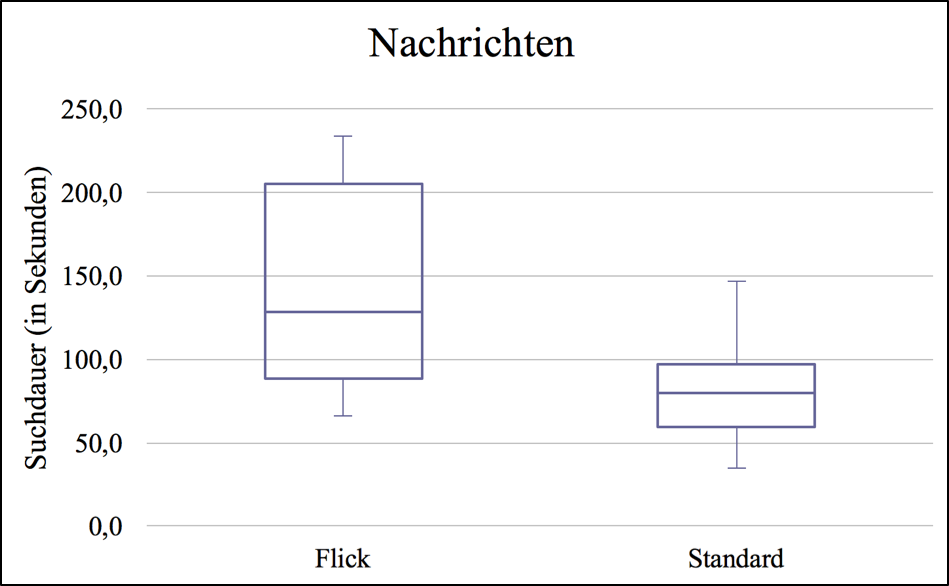
\includegraphics[scale=0.9]{./images/33.png}
\caption{Boxplot zur Suchdauer Nachrichten Videos}
\label{boxplot_nachrichten}
\end{center}
\end{figure}
Das nächste Video, welches als Teil der Untersuchung herangezogen wurde, war die Dokumentation. Auf Basis des Mittelwertes lässt sich hier ein großer Unterschied erkennen, denn die durchschnittlichen Suchzeiten beim Flickplayer liegen hier bei 128,81 Sekunden, bei einer Standardabweichung von  $\pm 90,33$. Die Durchschnittszeiten beim Standardplayer liegen mit 67,81 Sekunden mit einer Standardabweichung von $\pm 29,3$. Wenn man jedoch den Boxplot in Abbildung 5.4 genauer betrachtet, dann fällt auf, dass die Boxplotlänge, sowie dessen Position für beide Videoplayer eine ähnliche Lage haben, also der Großteil der Teilnehmer die Aufgaben in einem ähnlichen Zeitfenster abgeschlossen haben. Der Boxplot des Flickplayers zeigt aber, dass es Ausreißer gab, die sich negativ auf die durchschnittlichen Performanz der Applikation ausgewirkt haben. Auch hier wird wieder die Signifikanz mit dem Wilcoxon-Vorzeichen-Rang-Test untersucht. Der gelieferten Ergebnisse sind z = -2,7923 bei p = 0,05 und einer Summe der positive Ränge von 122, bzw. der negative Ränge von 14. Diese Ergebnisse lassen darauf schließen, dass es einen Unterschied gibt und dieser auch signifikant ist. Das bedeutet, dass auch hier der Standardplayer schneller als der Flickplayer war. Das bedeutet also, dass bei langen Videos die Suche von einer bestimmten Szene mit dem Standardplayer schneller ist, im Vergleich zur der Suche mit dem Flickplayer. Da dies die reinen statistischen Werte über die Performanz des Flickplayer sind, lassen sich damit keine Aussagen darüber treffen, wie die Testpersonen die Navigationsmethode subjektiv empfunden haben. Dies wird mit der Analyse der Fragebögen im weiteren Verlauf der Arbeit erörtert.
\begin{figure}[h]
\begin{center}
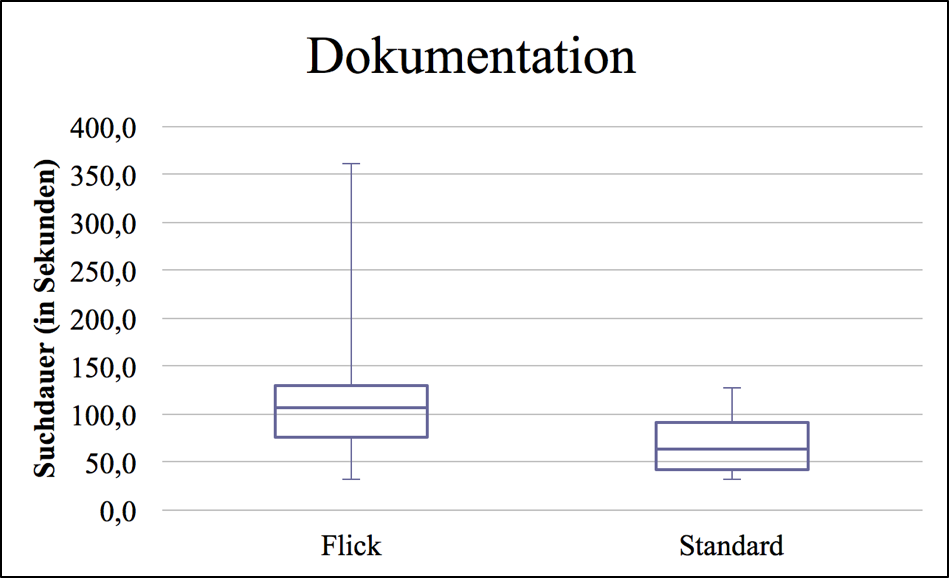
\includegraphics[scale=0.9]{./images/34.png}
\caption{Boxplot zur Suchdauer Dokumentation Videos}
\label{boxplot_dokumentation}
\end{center}
\end{figure}

Die gesammelten Daten von den Zählaufgaben werden im nächsten Kapitel analysiert und evaluiert.

\subsection{Zählaufgaben}

Bei den Zählaufgaben mussten die Nutzer ohne zeitliche Beschränkung die vorgegeben Ereignisse Zählen. Relevant waren hier für die Evaluierung zwei Faktoren, welche zum einen die benötigte Zeit war und zum anderen die Genauigkeit der Zahlen. Das erste Video ist der Ausschnitt aus der Wer wird Millionär Sendung. Die gesuchten Ereignisse waren die korrekten Antworten, also A, B, C oder D. Die durchschnittliche Zeit, die benötigt wurde, war beim Flickplayer 191,56 Sekunden mit einer Standardabweichung von $\pm 106,83$. Im Vergleich liegt die Zeit mit dem Standardplayer im Schnitt bei 140,81 Sekunden mit $\pm 108,07$. Wenn man den Boxplot betrachtet, dann fällt auf, dass die meisten Nutzer die Aufgaben mit dem Standardplayer die Aufgaben in einer ähnlichen Zeit beendet haben, jedoch Ausreißer mit ca. 450 Sekunden Suchdauer den Durchschnitt stark beeinflusst haben. Die Signifikanz wurde wieder mit dem Wilcoxon-Vorzeichen-Rang-Test ermittelt. Die Werte z = -2,6371 bei p = 0,05 und die Summer der positive Ränge mit 119, bzw. die Summe der negativen Ränge mit 17 lassen daraus schließen, dass es einen signifikanten Unterschied zwischen den Videoplayern gibt. Dieser Unterschied geht auch hier wieder zugunsten des Standardplayers.
\begin{figure}[h]
\begin{center}
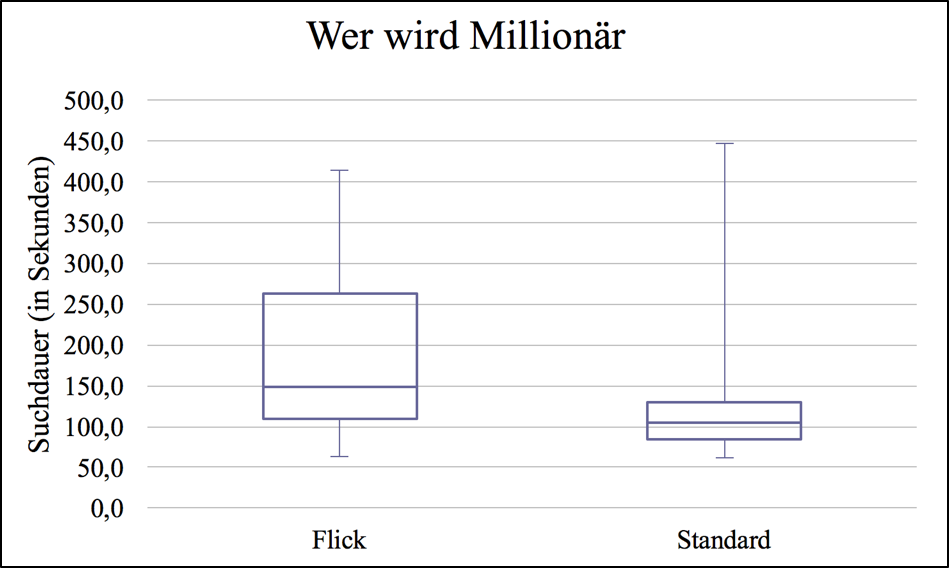
\includegraphics[scale=0.9]{./images/35.png}
\caption{Boxplot zur Suchdauer Quizshow Videos}
\label{boxplot_quizshow}
\end{center}
\end{figure}
Das nächste Video ist der Ausschnitt des Fußballspiels. Wie schon in einer der vorherigen Kapiteln erwähnt, mussten hier Ereignisse wie Mahnkarten, Tore, Einwürfe und Eckstöße gezählt werden. Die Durchschnittszeit beim Flickplayer liegt bei 336 Sekunden bei einer Standardabweichung von  $\pm 166,96$. Der die Probanden haben die Aufgaben mit dem Standardplayer in einer mittleren Zeit von 305,81 Sekunden bewältigt. Die Standardabweichung liegt bei dieser Messung bei  $\pm 202,85$. Die Boxplots in Abbildung 5.6 weisen eine sehr ähnliche Form bezüglich Form und Position auf. Wie die Durchschnittswerte schon angedeutet haben, sind die Suchzeiten bei dem Standardplayer leicht verkürzt. Die Resultate aus dem Wilcoxon-Vorzeichen-Rang-Test besagt mit einem p-Wert von 0,28434, welcher das Signifikanz-Niveau von p = 0,05 übersteigt, dass die Unterschiede nicht signifikant sind. Wie die Auswertung gezeigt hat, kann der Flickplayer den Nutzer nicht dabei unterstützen die Zählaufgaben schneller zu erledigen, als der Standardplayer, sondern unterliegt diesem. Eine weitere Annahme der Studie war, dass der Nutzer bei der Navigation mit dem Flickplayer mehr von dem Inhalt eines Video mitbekommt, also mit herkömmlicher Navigation. Daher sollte auch die Richtigkeit bzw. Genauigkeit der Zählwerte der Nutzer überprüft werden. Dafür wurde ein gewichtetes Modell erstellt, welches so funktioniert, dass die Anzahl der Nutzer ermittelt wird, welche alle Ereignisse gefunden haben, einen Fehler, zwei Fehler oder mehr als zwei Fehler gemacht haben. Für jeden Nutzer der die Aufgaben fehlerfrei beendet hat, bekommt der jeweilige Videoplayer 4 Punkte, für einen Fehler wird ein Punkt abgezogen, bei zwei Fehlern wird ein weiterer Punkt abgezogen, sodass bei mehr als zwei Fehlern nur noch ein Punkt vergeben wird. Somit ergibt sich eine maximale Punktzahl von 64 Punkten bei 16 Probanden. Die erreichten Punkten werden im Anschluss durch die maximale Punktzahl geteilt, sodass sich ein Prozentwert erhalten wird, welcher die Genauigkeit des jeweiligen Videoplayers repräsentiert. Der Flickplayer hat bei den Quizshow insgesamt 14 Nutzer gehabt, die die Aufgaben fehlerfrei beendet haben. Eine Gesamtpunktzahl von 61 wurde erreicht, was einer Genauigkeit von 95,31\% entspricht. Im Vergleich dazu hat der Standardplayer nur 52 Punkte erreicht, da nur 12 Personen alle Ereignisse richtig gezählt haben. Die Genauigkeit ist daher mit 84,36\% geringer verglichen zum Flickplayer.
\begin{figure}[h]
\begin{center}
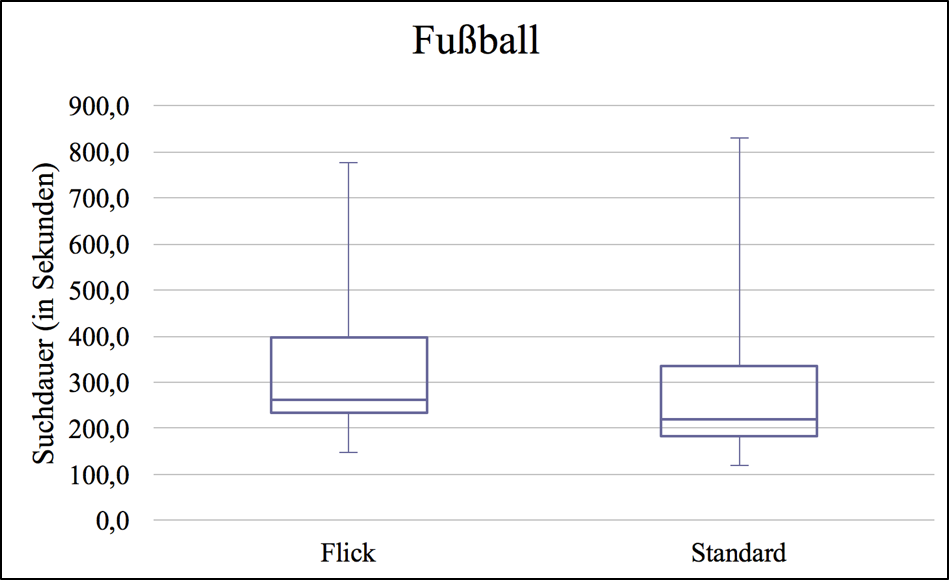
\includegraphics[scale=0.9]{./images/36.png}
\caption{Boxplot zur Suchdauer Fußball Videos}
\label{boxplot_fussball}
\end{center}
\end{figure}
Die Fußball-Videos wurden aus ausgewählt, da deren Schwierigkeitsgrad höher ist, verglichen zu den Quizshow-Videos, da die Ereignisse sind noch eindeutig sind und außerdem nicht alle Ereignisse an der selben Stelle im Video sind. Des Weiteren ist aufgrund von Wiederholungen bei einer schnellen Navigation nicht immer ganz klar, ob das selbe Ereignis mehrfach gezeigt wird, oder es sich um ein neues handelt. Die Gesamtpunktzahl, die durch den Flickplayer erreicht wurde liegt bei 49, da insgesamt nur 7 Personen alle Ereignisse richtig gezählt haben. Somit wurden insgesamt 76,56\% der maximalen Punkte erreicht. Den Gegenübergestellt steht der Standardplayer, welcher insgesamt nur 28 Punkte erreicht hat. Nur ein Personen haben fehlerfrei gezählt und 13 Personen hatten 2 oder mehr Fehler. Somit liegt die Genauigkeit bei 43,75\% und ist deutlich ungenauer als beim Flickplayer. Die Studie hat somit bestätigt, dass die Teilnehmer mit dem Flickplayer zwar länger gebraucht haben, um die Zählaufgaben zu lösen, jedoch haben mehr vom Inhalt aufgenommen haben.

Im folgenden Kapitel wird die subjektive Wahrnehmung der Probanden untersucht, um festzustellen, ob die Navigationsmethode des Flickplayers einen positiven Eindruck gegeben hat, im Vergleich zum Standardplayer mit Zeitleistennavigation.

\subsection{Benutzerbewertung im NASA TLX}

Wie Kapitel schon 5.2 schon erwähnt wurde, basiert der erste Teil des Fragebogens auf dem NASA-TLX, welcher häufig eingesetzt wird, um die Effektivität von Systemen zu testen. Dabei werden insgesamt 6 Fragen gestellt, von der jede eine Bewertung auf einer Intervallskala von 1 bis 21 vorgibt, wobei 1 immer eine niedrigere Belastung und 21 das andere Extrem bedeutet. Jedoch im Falle von Frage 4 bedeutet 1, dass die Aufgabe perfekt gelöst wurde und 21, dass der Nutzer gescheitert ist. Die Fragen lauten im Einzelnen wie folgt:
\begin{enumerate}
\item	Wie anspruchsvoll waren die Aufgaben auf mentaler Ebene?
\item	Wie körperlich anspruchsvoll waren die Aufgaben?
\item	Wie hoch war der zeitliche Druck beim Erledigen der Aufgaben?
\item	Wie erfolgreich haben Sie die gestellten Aufgaben erledigt?
\item	Wie stark mussten Sie sich anstrengen, um die Aufgaben zu erledigen?
\item	Wie unsicher, irritiert, gestresst, entmutigt und genervt waren Sie bei der Durchführung der Aufgaben?
\end{enumerate}
Alle Probanden haben diesen Fragebogen für jeden Videoplayer einmal ausgefüllt und zwar immer direkt nach dem Erledigen der Aufgaben mit der jeweiligen Applikation. Der Grund hierfür war, dass die Eindrücke so am frischsten sind. Um nun herauszufinden, ob einer der Videoplayer statistisch gesehen besser ist, als der andere, wurde für jede einzelne Frage der Wilcoxon-Vorzeichen-Rang-Test durchgeführt. Die bietet sich an, da sich die gelieferten Werte zu Stichprobenpaare kombinieren lassen und auf deren Basis festzustellen, ob es einen Unterschied zwischen den beiden Videoplayern gibt und wenn ja, ob dieser signifikant ist.
\begin{figure}[h]
\begin{center}
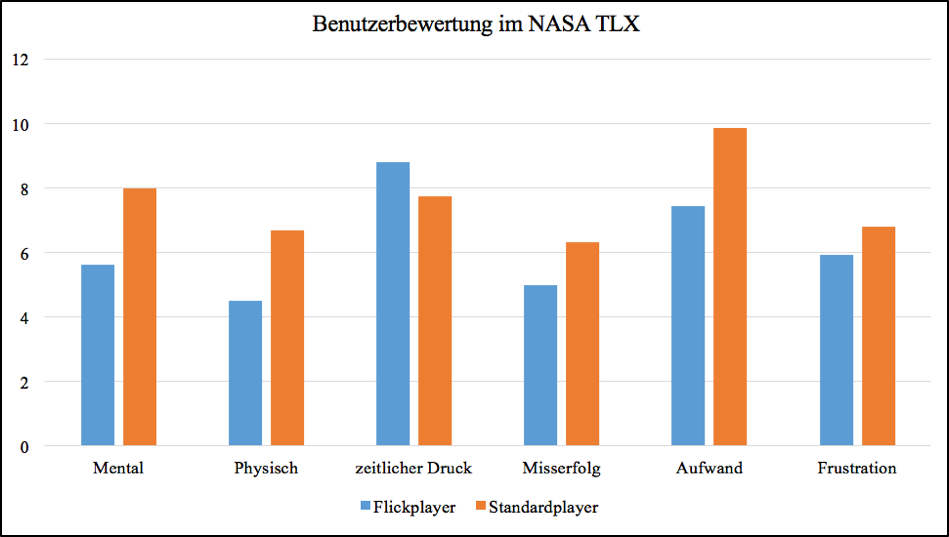
\includegraphics[scale=0.9]{./images/37.png}
\caption{NASA TLX Bewertungsverteilung von 1 - 21}
\label{nasa_tlx}
\end{center}
\end{figure}
In der unteren Abbildung 5.7 sind die durchschnittlichen Bewertungen durch die Teilnehmer zu sehen. Ein niedriger Wert bedeutet, dass die Belastung bspw. eher geringer war, was ein positiver Faktor für einen Videoplayer ist. Man kann auf dem Diagramm schnell erkennen, dass der Flickplayer im Vergleich zum Standardplayer bei den meisten Dimensionen eine im Durchschnitt besser Bewertung erhalten hat. Der zeitliche Druck beim ausführen der Aufgaben war der einzige Faktor, bei dem der Standardplayer scheinbar einen Vorteil hatte. Die Auswertung des Wilcoxon-Vorzeichen-Rang-Test ergab, dass die Unterschiede beider Stichproben bei den Fragen bezüglich des zeitlichen Drucks und der Frustration mit z = -0,3844 und z = -1,0225 zwar gegeben ist, dieser aber bei p = 0,05 nicht signifikant war. Die weitere Untersuchung auf die Frage der mentalen Belastung hat ergeben, dass bei z = -2,1344 und p = 0,05 der Flickplayer eine geringere Belastung hat und der Unterschied signifikant ist. Die Physische Belastung hat ebenfalls einen signifikanten Unterschied zugunsten des Flickplayers mit z = -2,4006 und p = 0,05. Bei den Fragen 4 und 5 zum Thema Misserfolg und betriebener Aufwand hat auch hier wieder der Flickplayer einen signifikanten Unterschied im Vergleich zum Standardplayer, mit z = -2,1972 und z = -2,6052 mit jeweils und p = 0,05.

\subsection{Bevorzugter Videoplayer}

Ein Teil des Fragebogens war es auch herauszufinden, welcher Videoplayer den Nutzern subjektiv besser gefallen halt. Um dies zu ermitteln, sollten die Teilnehmer zum einen beide Videoplayer anhand einer Schulnotenskala von 1 – 6 bewerten, wobei die die beste Note und 6 die schlechteste Note ist. Des Weiteren gab es ein Textfeld, in der die Nutzer weitere Kommentare schreiben konnten, um explizitere Aussagen treffen zu können. Die folgende Grafik zeigt die Verteilung der einzelnen Benotungen durch die Probanden.
\begin{figure}[h]
\begin{center}
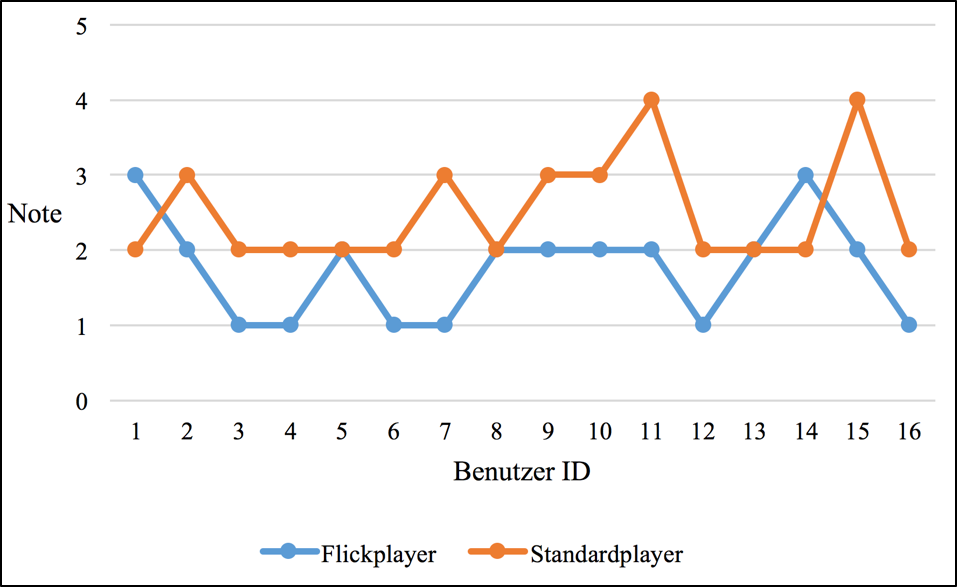
\includegraphics[scale=0.9]{./images/38.png}
\caption{Subjektive Bewertung der Videoplayer}
\label{benotung}
\end{center}
\end{figure}
Die blaue Linie repräsentiert die Noten des Flickplayers und die orangene Linie die des Standardplayers. Hier ist leicht zu erkennen, dass die Noten des Flickplayers in den meisten Fällen besser ist, im Vergleich zu den Bewertungen des Standardplayers. Im Durchschnitt haben die 16 Teilnehmer eine Note von 1,75 für den Flickplayer geben, mit einer Standardabweichung von  $\pm 0,66$ und für den Standardplayer eine Durchschnittsnote von 2,5 mit einer Standardabweichung von  $\pm 0,7$. In 11 von 16 Fällen haben die Probanden den Flickplayer dem Standardplayer eindeutig vorgezogen, was 68,75\% entspricht. Allerdings muss hier hervorgehoben werden, dass in den anderen 5 Fällen der Standardplayer nicht immer als präferierter Videoplayer genannt werden kann, sondern in 3 Fällen beide Videoplayer eine gleiche Benotung erhalten haben und nur 2 Probanden den Standardplayer vorgezogen haben. Die Auswertung der schriftlichen Anmerkungen hat ergeben, dass die Nutzer insbesondere die permanente Interaktion mit der Navigationsleiste beim Standardplayer negativ bewerten. Sie mussten sich sehr darauf konzentrieren, dass sie den Schieberegler nicht zu schnell bewegen und somit die Aufmerksamkeit nicht auf den Inhalt des Videos gerichtet wird. Des Weiteren wurde bemängelt, dass die Position der Navigationsleiste am oberen Bildschirmrand ist und dadurch die Hand während der Interaktion das Video bedeckt und eine schiefe Haltung erforderlich wurde. Im Gegensatz dazu wurde dies beim Flickplayer hervorgehoben, dass die Folgen einer Wischgeste auch noch dann einen Einfluss auf die Navigation haben, wenn die Hand vom Bildschirm genommen wird. Dadurch war der Gesamteindruck, dass die Navigation auf dem Flickplayer weniger anstrengend ist in Bezug auf den körperlichen Aufwand.

Das folgende Kapitel bildet mit der Schlussfolgerung und dem Ausblick für die Zukunft den Schluss dieser Arbeit.

\chapter{Resümee und Ausblick}

In der heutigen Zeit zeigt der Konsum von Videos eine enorm steigende Entwicklung. Smartphones und Tablets tragen hierbei eine erhebliche Rolle für das Wachsen von privaten Video-Bibliotheken. Die Herausforderung ist es diese Videos und Sammlungen für die Nutzer zugänglich zu machen, sodass diese auch wiedergefunden werden. Die vorliegende Arbeit untersuchte die Thematik von Videobrowsing insbesondere im mobilen Sektor. Einige Applikationen für den Desktop-Bereich sind bereits erfolgreich für Tablets und Smartphones angepasst worden, jedoch gibt es keine weitverbreitete Alternativen zu Videoplayern mit einer Zeit-basierten Suchleiste. Leichte Anpassungen wie Vorschaubilder auf der Navigationsleiste sind jedoch keine Seltenheit bei bekannten Videoportalen wie YouTube.

Auf der Grundlage von existierenden mobilen Videoplayern, wie dem SwiPlayer, wurde eine Videoapplikation vorgeschlagen, welche mit Hilfe von Wischgesten ein Video in stark beschleunigter Abspielrate wiedergibt. Dadurch sollte es für den Betrachter einfacher sein, schnell einen Überblick über den Inhalt des Videos zu erhalten. Aufgrund von Granularität von mehreren Geschwindigkeitsstufen, die eng mit der Wischgesteninteraktion verbunden ist, sollte dem Nutzer ein positives Benutzererlebnis geboten werden. 

Bei der Entwicklung des Flickplayers lagen die Hauptprobleme vor allem bei den eingeschränkten Ressourcen. Ein Video in bis zu 32-facher Geschwindigkeit abzuspielen, ohne auf eine flüssige Wiedergabe zu verzichten, war nicht möglich. Daher mussten Wege gefunden werden dieses Problem zu kaschieren. Eine für den Produktivgebrauch nicht geeignete Lösung war es, ein Video in drei verschiedenen Geschwindigkeiten zu kodieren und diese übereinanderzulegen. Somit konnte durch schnelles Schalten zwischen den Videos und kontinuierliches synchronisieren der Eindruck vermittelt werden, dass es sich nur um ein einzelnes Video handelt. Da das Ziel dieser Arbeit die Entwicklung und Evaluierung der Wischgesteninteraktion ist, konnte dieser Kompromiss eingegangen werden.

Die Fragestellung, ob eine derartige Navigationsmethode von Vorteil ist, wurde im Rahmen einer Benutzerstudie mit 16 Teilnehmern ermittelt. Verschiedene Aufgaben aus dem Bereich known-item search und einer Zählsuche sollte Aufschluss darauf geben, ob der Flickplayer in Gegenüberstellung zu einem Standardplayer eine bessere Unterstützung bietet. Die Analyse der gewonnenen Daten hat ergeben, dass in fast allen Fällen die Probanden mit dem Standardplayer die Aufgaben signifikant schneller fertiggestellt haben. Dies war sowohl bei den Zielsuchaufgaben, sowie bei der Zählsuche der Fall. Zusätzlich wurde bei den Zählsuchaufgaben auch die Genauigkeit der gezählten Ereignisse ausgewertet. Hier wurde sehr deutlich, dass die Nutzer mit dem Flickplayer generauere Endergebnisse erzielen konnten und insgesamt die Ereignisse besser erkannt und sich weniger häufig verzählt haben. Als Teil der Benutzerstudie hat jeder Teilnehmer im Anschluss für beide Videoplayer Applikationen einen Bewertungsbogen ausgefüllt, welcher auf dem NASA TLX Fragebogen basierte. Die gewonnenen Daten besagen, dass die Nutzer mit dem Flickplayer eine geringere mentale und physische Belastung erlebten. Ebenso das Frustniveau und das Empfinden von Misserfolg konnte der Flickplayer niedriger halten, verglichen mit dem Standardvideoplayer. Eine subjektive Benotung durch die Teilnehmer ergab, dass fast 68\% den Flickplayer für das Bearbeiten der Aufgaben bevorzugten, obwohl sie damit mehr Zeit benötigten. Besonders hervorgehoben wurde, dass die Wischgesteninteraktion intuitiv sei und es dem Nutzer einfacher machte sich auf den Inhalt der Videos zu konzentrieren.

Auf Grundlage der gewonnenen Erkenntnisse durch die Studie kann gesagt werden, dass in Wischgesten vom Nutzer akzeptiert werden, jedoch diese spezielle Navigationsmethode keine kürzeren Suchzeiten bewirkte. In Zukunft sollten daher weitere Forschung in diesem Bereich betrieben werden, bei der die Konzepte von traditioneller Navigationsleisten mit Wischgesteninteraktion kombiniert werden. Somit könnte das Benutzererlebnis für die breite Masse verbessert werden ohne Einbüßen bei der Suchgeschwindigkeit zu machen.















%	\bibliographystyle{plain} %nummerierung in der reihenfolge wie bib-file
%	\bibliographystyle{abbrv} %wie plain, namen werden abgekuerzt
\bibliographystyle{unsrt} %keine sortierung - durch \cite vorgegeben
%	\bibliographystyle{alpha} %nummer aus autorenkuerzel und jahr wird erzeugt
\addcontentsline{toc}{chapter}{Literatur}



\bibliography{references}
\clearemptydoublepage
\addcontentsline{toc}{chapter}{Appendix}
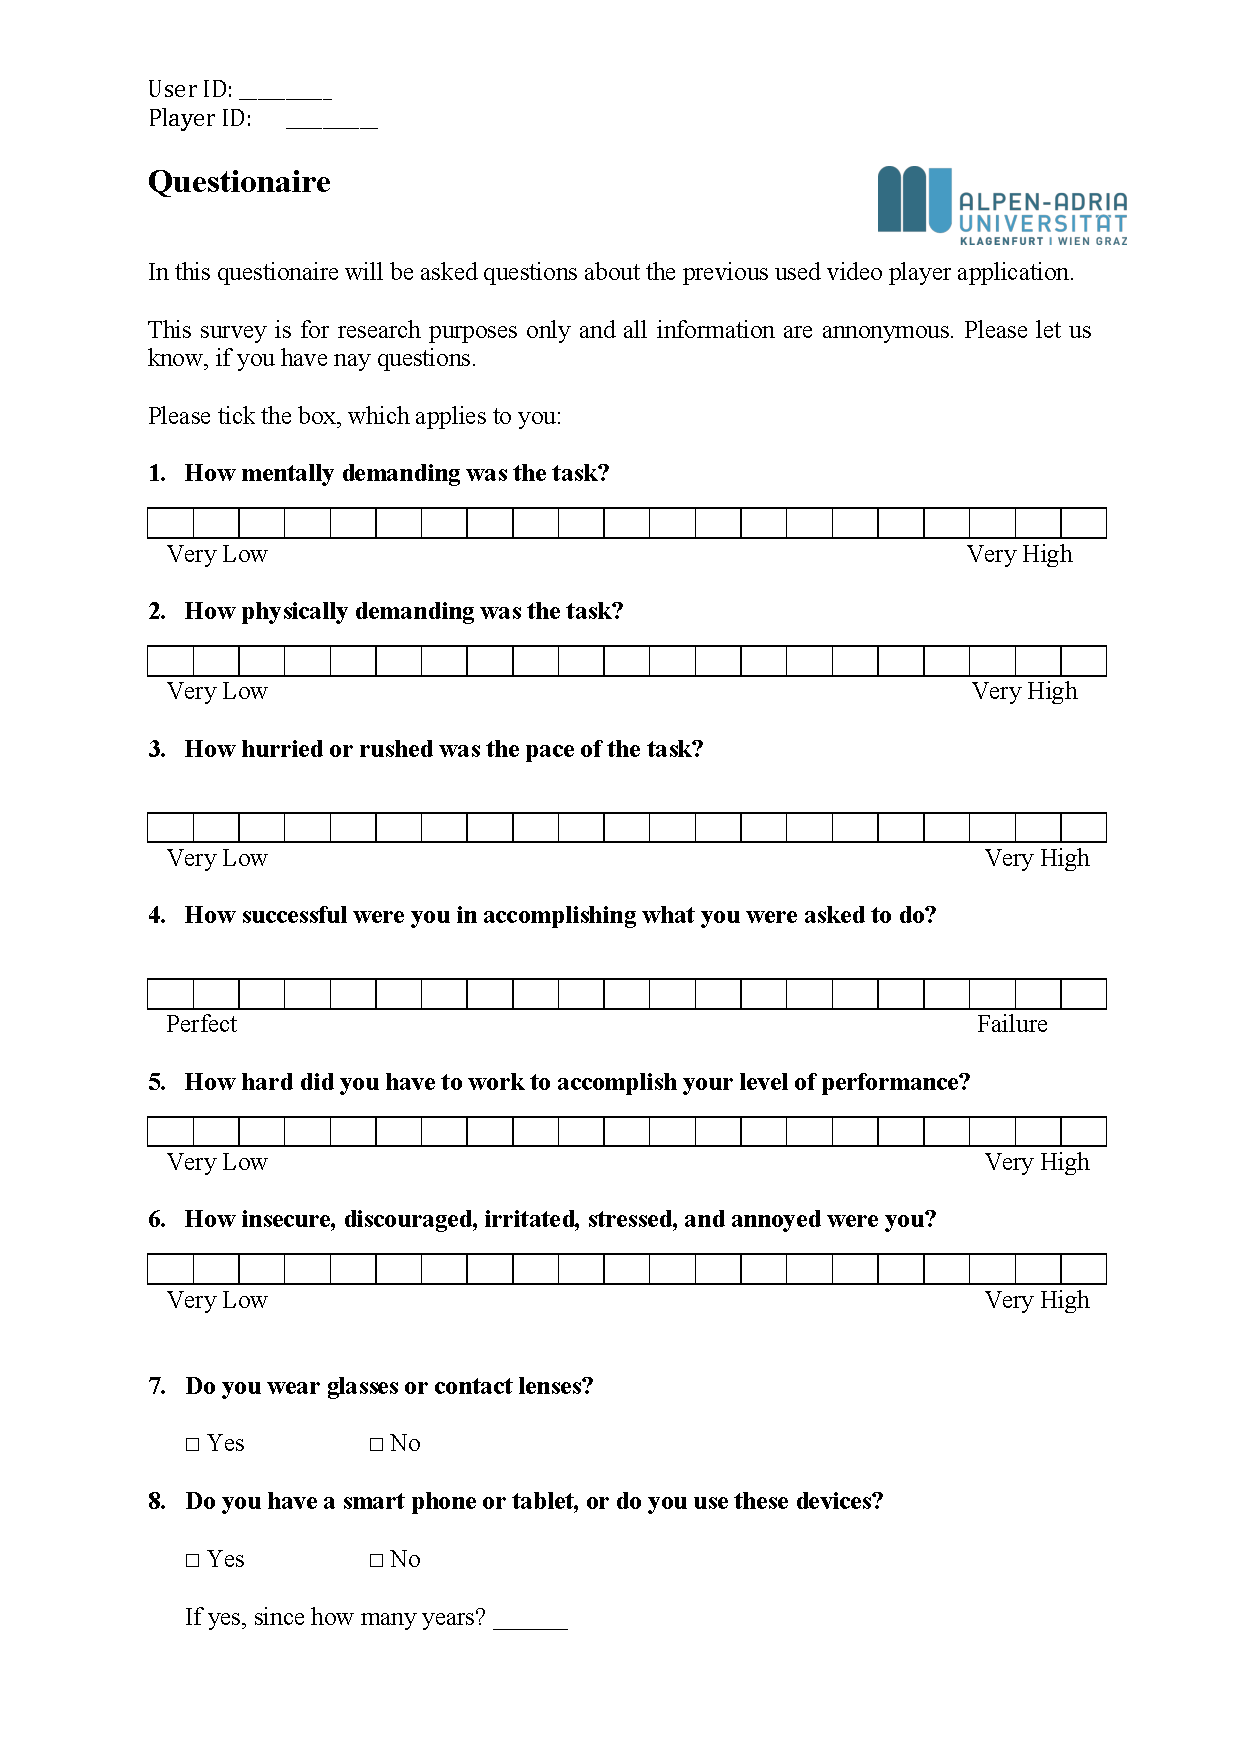
\includepdf[pages=-]{Fragebogen_2_en}
	
%	\printindex
%	\printglossary

\end{document}

